%%%%%%%%%%%%%%%%%%%% book.tex %%%%%%%%%%%%%%%%%%%%%%%%%%%%%
%
% sample root file for the chapters of your "monograph"
%
% Use this file as a template for your own input.
%

% RECOMMENDED %%%%%%%%%%%%%%%%%%%%%%%%%%%%%%%%%%%%%%%%%%%%%%%%%%%
\documentclass[graybox,envcountchap,sectrefs]{svmono}
% !TEX root = ./notes_template.tex

\usepackage{luatex85}
% \usepackage[all]{xy}

%\renewcommand{\baselinestretch}{1.05}
% amsthm omitted: svmono.cls already loads ntheorem and defines \theoremstyle
\usepackage{amsmath,amssymb,mathrsfs,amsfonts,dsfont}
\usepackage{epsfig,graphicx}
\usepackage{csquotes}
\usepackage{tabularx}
\usepackage{tablefootnote}
\usepackage{longtable}
\usepackage{blkarray}
\usepackage{slashed}
\usepackage{color}
\usepackage{listings}
\usepackage{caption}
% \usepackage{fullpage}
\usepackage{lipsum} % provides dummy text for testing
\usepackage[toc,title,titletoc,header]{appendix}
%\usepackage{minitoc}
\usepackage{color}
\usepackage{float}
\usepackage{multicol} % two-col ToC
\usepackage{bm}
\usepackage{imakeidx} % before hyperref
\usepackage{hyperref}
\hypersetup{
    colorlinks=true,
    citecolor=magenta,
    linkcolor=blue,
    filecolor=green,      
    urlcolor=cyan,
    % hypertexnames=false,
}
\usepackage[capitalise]{cleveref}
\usepackage{subcaption}
\usepackage{enumitem}
\usepackage{mathtools}
\usepackage{physics}
\usepackage[linesnumbered,ruled,vlined,algosection]{algorithm2e}
\usepackage{movie15}
\usepackage{wrapfig}
\usepackage{comment}

\SetCommentSty{textsf}

\topmargin-1.2cm
% \headheight0.0cm
\headheight13.6pt
\headsep1.2cm
\oddsidemargin0.0cm
\evensidemargin0.0cm
\textheight23.0cm
\textwidth16.9cm
\footskip1.0cm





%%%%%%%%%%%%%%%% ToC %%%%%%%%%%%%%%%%%%%%%
% Link Chapter title to ToC: https://tex.stackexchange.com/questions/32495/linking-the-section-text-to-the-toc
\usepackage[explicit]{titlesec}
\titleformat{\chapter}[display]
  {\normalfont\huge\bfseries}{\chaptertitlename\ {\thechapter}}{20pt}{\hyperlink{chap-\thechapter}{\Huge#1}
\addtocontents{toc}{\protect\hypertarget{chap-\thechapter}{}}}
\titleformat{name=\chapter,numberless}
  {\normalfont\huge\bfseries}{}{-20pt}{\Huge#1}

%%%%%%%%%%%%%%%%%%% fancyhdr %%%%%%%%%%%%%%%%%
\usepackage{fancyhdr}
\pagestyle{fancy} % enable fancy page style
\renewcommand{\headrulewidth}{0.0pt} % comment if you want the rule
\fancyhf{} % clear header and footer
\fancyhead[lo,le]{\leftmark}
\fancyhead[re,ro]{\rightmark}
\fancyfoot[CE,CO]{\hyperref[toc-contents]{\thepage}}

% https://tex.stackexchange.com/questions/550520/making-each-page-number-link-back-to-beginning-of-chapter-or-section
\makeatletter
\def\chaptermark#1{\markboth{\protect\hyper@linkstart{link}{\@currentHref}{Chapter \thechapter ~ #1}\protect\hyper@linkend}{}}
\def\sectionmark#1{\markright{\protect\hyper@linkstart{link}{\@currentHref}{\thesection ~ #1}\protect\hyper@linkend}}
\makeatother
%%%%%%%%%%%%%%%%%%% fancyhdr %%%%%%%%%%%%%%%%%


%%%%%%%%%%%%%%%%%%% biblatex %%%%%%%%%%%%%%%%%
%\usepackage[doi=false,url=false,isbn=false,style=alphabetic,backend=biber,backref=true]{biblatex}
\usepackage[natbib,style=alphabetic,refsection=chapter]{biblatex}
\addbibresource{references.bib}

\newbibmacro{string+doiurlisbn}[1]{%
  \iffieldundef{doi}{%
    \iffieldundef{url}{%
      \iffieldundef{isbn}{%
        \iffieldundef{issn}{%
          #1%
        }{%
          \href{http://books.google.com/books?vid=ISSN\thefield{issn}}{#1}%
        }%
      }{%
        \href{http://books.google.com/books?vid=ISBN\thefield{isbn}}{#1}%
      }%
    }{%
      \href{\thefield{url}}{#1}%
    }%
  }{%
    \href{http://dx.doi.org/\thefield{doi}}{#1}%
  }%
}

% https://tex.stackexchange.com/questions/94089/remove-quotes-from-inbook-reference-title-with-biblatex
\DeclareFieldFormat[article,incollection,inproceedings,book,misc]{title}{\usebibmacro{string+doiurlisbn}{\mkbibemph{#1}}}
% https://tex.stackexchange.com/questions/454672/biblatex-journal-name-non-italic
\DeclareFieldFormat{journaltitle}{#1\isdot}
\DeclareFieldFormat{booktitle}{#1\isdot}
% https://tex.stackexchange.com/questions/10682/suppress-in-biblatex
\renewbibmacro{in:}{}
% add video field: https://tex.stackexchange.com/questions/111846/biblatex-2-custom-fields-only-one-is-working
\DeclareSourcemap{
    \maps[datatype=bibtex]{
      \map{
        \step[fieldsource=video]
        \step[fieldset=usera,origfieldval]
    }
  }
}
\DeclareFieldFormat{usera}{\href{#1}{\textsc{Online video}}}
\AtEveryBibitem{
    \csappto{blx@bbx@\thefield{entrytype}}{% put at end of entry
        \iffieldundef{usera}{}{\space \printfield{usera}}
    }
}
%%%%%%%%%%%%%%%%%%% biblatex %%%%%%%%%%%%%%%%%


% choose options for [] as required from the list
% in the Reference Guide

%\usepackage{mathptmx}
%\usepackage{helvet}
%\usepackage{courier}
%
\usepackage{type1cm}         

\usepackage{makeidx}         % allows index generation
\usepackage{graphicx}        % standard LaTeX graphics tool
                             % when including figure files
\usepackage{multicol}        % used for the two-column index
\usepackage[bottom]{footmisc}% places footnotes at page bottom

\usepackage{newtxtext}       % 
\usepackage{newtxmath}       % selects Times Roman as basic font
% svmono.cls already defines \c@minitocdepth for its own purposes;
% clear it first so the real minitoc package can define its own counter.
\makeatletter
\let\c@minitocdepth\relax
\makeatother
\usepackage{minitoc}

% see the list of further useful packages
% in the Reference Guide

\makeindex             % used for the subject index
                       % please use the style svind.ist with
                       % your makeindex program

%%%%%%%%%%%%%%%%%%%%%%%%%%%%%%%%%%%%%%%%%%%%%%%%%%%%%%%%%%%%%%%%%%%%%

\graphicspath{{./}{images/}}

\begin{document}

\author{}

\title{Clinical Physiology}
\subtitle{A muscle centered approach \\ \\ \\ -- version 4 -- \\ \\ \\ \normalsize{Sean Collins} \\ \normalsize{Professor of Clinical Inquiry} \\ \\ \normalsize{Doctor of Physical Therapy Program} \normalsize{Plymouth State University} }

\maketitle

%--copyright--------------------------------------------------
\pagebreak
\thispagestyle{empty}
\begin{flushleft}
%{\small
Copyright \copyright 2025 Sean Collins \\

\vspace{0.2in}

ISBN (eBook): 979-8-9907667-0-9 \\
ISBN (Paperback): 979-8-9907667-1-6

\vspace{0.2in}

PT Centered Press       \\
Ashland, NH, 03217

\vspace{0.2in}

Permission is granted to copy, distribute, and/or modify the text of this document under the terms of Creative Commons BY-NC-SA 4.0 DEED
Attribution-NonCommercial-ShareAlike 4.0 International, which is available at \url{https://creativecommons.org/licenses/by-nc-sa/4.0/deed.en}. This copyright only refers to the text of the book. Restrictions exist for figures rendered with BioRender and for permission to use any figure created with BioRender please contact the author for details. Permission to recreate a figure, capturing its essential concepts for example, is given through the CC BY-NC-SA 4.0 DEED license, but use of an exact figure which has been created in BioRender is restricted by the terms of the authors BioRender Academic License. In such instances this will require the requester to secure their own BioRender Account and follow the terms of that account.

\vspace{0.2in}

The original form of this book is \LaTeX\ source code.  Compiling this \LaTeX\ source has the effect of generating a device-independent representation of a textbook, which can be converted to other formats and printed. The code that developed this book is stored in a GitHub repository and can be made available upon request to the author at: scollinspt@tuta.com

\end{flushleft}

\vspace{0.2in}

%} end small

%---end--copyright--------------------------------------------------------

\frontmatter%%%%%%%%%%%%%%%%%%%%%%%%%%%%%%%%%%%%%%%%%%%%%%%%%%%%%%


%%%%%%%%%%%%%%%%%%%%%%% dedic.tex %%%%%%%%%%%%%%%%%%%%%%%%%%%%%%%%%

\begin{dedication}

\begin{flushleft}

To God, for sustaining grace and the mystery of the ultimate questions. 
To my parents, Nancy and Joe, for instilling in me the gift of pragmatism and wisdom to navigate life’s complexities. \\
To my sons, Tim \& Andrew—For showing me, beyond all doubt, the meaning of unconditional love. \\ 
To my friend Gary for challenging me to think deeper and engage with the ultimate questions of existence. \\
To my wife, Traci, for grounding me in the reality where those ultimate questions truly matter. \\

\end{flushleft}

\end{dedication}





%\include{author/foreword}

\preface

Clinical Physiology: A muscle centered approach is a manuscript (book) in progress. The version you are reading was released \today.

\vspace{0.2in}

This project emerged late in my sabbatical year, early April 2022. I had been working on a book for my course sequence titled \textit{Clinical Inquiry} and was unable to break through some theory to practice barriers. I had been meeting for weekly discussions with my friend Bog Sniezek, who is a systems scientist that was at Draper Labs in Cambridge and is now a consultant for the Air Force. During our conversation about the nature and function of unifying systems (Bog's theory), he inspired some thoughts about how physical therapists should learn clinical physiology. It is a foundational knowledge for all areas of practice. The idea that struck me on the basis of unifying systems theory was a muscle-centered approach. From the perspective of a physical therapist, physiology is the generative (muscle cell) and supportive (other systems) role in movement. The tension developed by muscles, which is developed by muscle cells, is at the core of movement. Muscle cells developing tension are a necessary but not sufficient condition for movement. Muscles have always been included in the clinical physiology course that I teach. In fact, there is no new material in the book from the perspective of what is being taught. The only thing new is that all things are considered from the perspective of the muscle fiber. Since my sabbatical was close to completion and I did not have a draft of my original plan (a book on clinical inquiry) and I had a \textit{Clinical Physiology} course to teach in a couple of months; I made the decision to start working on this text. In my 30-year history of teaching this topic, I was never satisfied with the textbook options. It was a Goldilocks situation. I either spent class time explaining to students what they did not need to know and adding topics related to movement to a medical physiology textbook; or I spent time adding clinical topics to an exercise physiology textbook. Either way, it discouraged students from reading the book and focusing on the lectures. However, the lectures were dense and students would often say things such as: \textit{"I wish I had a transcript of the lecture."} This book is a transcript of those lectures. A secondary goal of this book is that students will learn how to learn through graduate level academic reading.

\vspace{0.2in}

A muscle-centered approach places the muscle fiber (cell) at the center of the inquiry. \textbf{Part I} establishes preliminaries to put muscle fiber in context.  \textbf{Part II} focuses on what a muscle fiber does as a system. Muscle fibers create tension, a specific type of force. The process of creating tension is an inward looking process. We consider the cellular, mechanical, and chemical mechanisms of the muscle fiber. \textbf{Part III} focuses on the necessary supporting systems for muscle fiber. Each muscle fiber receives and releases material from its surrounding environment (extra cellular fluid). Several physiological systems are integrated to ensure the stability of that environment. Parts I through III are covered in the author's DPT course, \textit{Clinical Physiology}, at Plymouth State University.

\vspace{0.2in}

\textbf{Part IV} (in progress) will focus on muscle molecular biology. Specifically, how the muscle continues to fulfill its role of creating tension without being a burden on the physiological support systems. Topics include atrophy, hypertrophy, and repair. \textbf{Part V} (in progress) will include a variety of integrated exercises. These topics have been selected to highlight the need for physiological coordination.

\subsection*{Clinical Physiology in a DPT curriculum}
A DPT program has the challenge of educating individuals of diverse backgrounds in the core set of knowledge to become physical therapists. Clinical physiology is a foundational knowledge. The book fits best in a first term course, or a first course on human physiology. The book assumes that the reader has taken prerequisite courses in anatomy \& physiology, physics, and chemistry. It is not an exercise physiology text, though it has a lot of content that would be found in an exercise physiology text. It is not a medical physiology text, though it has a lot of content that would be found in a medical physiology text. The book includes a foundational knowledge of the physiology for a physical therapist. That knowledge is buried in a previously undiscovered textbook space that combines exercise physiology and medical physiology. 

\section*{Tips for the Reader \& Student}
Read actively. Question what you read as you read. Engage in what you read while you read. Every chapter begins with a brief introduction to orient your mind towards what you will be reading about; a mini table of contents so you can see the general layout; and objectives for you to start to think about what you will be learning. It is recommended that you start by reading these and then skim the rest of the chapter as a second step. This process helps you to read actively. During your pre-read skim, you should make mental note of the headings, subheadings, figures, and equations. The purpose of skimming is to get a sense of what is coming up as you start reading the chapter. When you start reading, read as if you were listening to the author speak. If you get a question in your head as you listen to me, write it down. Proceed to read even if you are not completely sure you understand what you are reading. Sometimes, a concept becomes clearer as you proceed. If not, make note of what you are not understanding and bring it to class. Identifying and clearing confusion is one of the purposes of class time; the second purpose of class time is application, depth, and breadth.

Each chapter ends with a summary that includes the \textit{Next Steps} to help you understand what has been covered and where we are headed. At the end of each chapter you will also find sample questions. You should be comfortable answering these questions. But you should also be comfortable manipulating them, turning them into other versions, making them easy or hard multiple choice questions based on the response options. Often the difficulty of a multiple choice question is not the question, the neighbors of the correct response option. Use the review questions to drive discussions during group study time. Yes, study in groups. Group study is the only thing you can do beyond class time to make sure you are not stuck in your own biased trap of understanding. You do not know what you do not know. You need others to bring you from unconscious incompetence to conscious incompetence, the first step towards conscious competence. 

\section*{A Note about Chapter Objectives}

The chapter objectives include specific behavioral terms. There is an ordered relationship between the behavioral terms that represents increasing and nested expectations. 

To \textbf{define} is to know the words being used and to know what they represent. Whether you can define something can be tested with a straightforward question such as identifying the correct definition from a set of definitions; whether you can write the definition; respond true or false to a proposed definition for a term; or identify the correct term from a set of terms when presented with a definition. 

To \textbf{explain} goes beyond defining, but it also implies that you can define the required terms. Explaining is the act associated with understanding. If you understand something, you can explain it. Objectives are typically written as acts - what the person learning can do if they have achieved the objective. Since understanding is observed as an act of explaining, we will use the objective "explain" when there is something that you must "understand". How do you demonstrate that you understand? You explain what it is that you understand. To explain, simultaneously holding a set of definitions together includes their relationship to each other. You can explain a model by demonstrating that you know all the definitions involved and describe how they relate to each other and that you can communicate that explanation. Whether you can explain something can be tested by asking about several aspects of what you are to explain or asking you to infer which part is missing; or by asking about one part and asking you to infer the other part. The point is to explain, which goes beyond defining and has an expectation of definition. But to define does not require you to explain. 

To \textbf{evaluate} requires you to make judgments and infer beyond the thing you are asked to evaluate. To evaluate implies that you can define and explain the thing (or concept) you are asked to evaluate. Being tested for whether you can evaluate can include asking you to infer to or from something that has not been directly covered or discussed, going beyond the thing (or concept) you are asked to evaluate to consider its implications in different situations. 

\textbf{Providing an example} is an objective based on a specific task and is considered a form of asking you to evaluate since it goes beyond a particular thing (or concept) to a totally new thing (or concept). Asking you to provide an example of a model requires you to know the concept of a model well enough that you can use your background knowledge to come up with something you are already familiar with that fits what you know about models. That level of knowledge requires you to evaluate a model because you evaluated your background knowledge and determined that it is a model. If a chapter objective asks you to provide an example of a model that is useful to physical therapy practice, it assumes that you will be able to define, explain, and evaluate the concept of a model and that you have background knowledge about physical therapy practice that you can use to evaluate models used in practice to consider what those models are and whether they are useful. Providing an example is similar to the objective \textbf{Apply}. With both of these objectives, you are asked to use your knowledge of the general concept (or thing) to a specific instance. If the concept was fruit, then an example is an apple. You can also apply the concept of fruit by listing several fruits, including what makes them all fruits.

\textbf{Compare and contrast} is also an objective based on a specific task that requires evaluation of two (or more) things (or concepts) to identify what is similar and different about them. This can occur with the general concept (e.g., fruit) by comparing fruits with vegetables, or with specifics (apples) by comparing different specific fruits (apples and oranges), or by comparing different specifics from each concept (apples and broccoli). Comparison and contrasting are an important higher-level evaluative process that helps you develop a deeper understanding.

\section*{Updates to the Third Version}

The third draft of this manuscript is now released as a **single PDF** as opposed to separate chapters. Therefore, it comes complete with **front matter** (though no back matter). Each chapter now has a **summary** as well as a few (**at least five**) sample questions at the end of the chapter.  

This draft is still not a completed manuscript, but is ready to receive **feedback from colleagues for peer review and possible submission to publishers.  

I had hoped to complete a glossary, an index, and improved contextual links between chapters**, but alas, these are deferred to a future draft.  

\section*{Updates to the Fourth Version}

This fourth version of the manuscript marks another step toward completion. It remains a single PDF, now with both front matter and back matter included.  

There are two new chapters:
\begin{itemize}
  \item The first completes \textbf{Part III: Muscle Support} and focuses on \textbf{digestion, absorption, and metabolism}.
  \item The second is the first chapter in \textbf{Part IV: Integration}, covering \textbf{Fick’s equation}.
\end{itemize}

I have expanded the \textbf{sample questions and added reflection questions} at the end of each chapter to reinforce key concepts. This draft has now undergone \textbf{peer review}, and I have decided to keep it perpetually as an \textbf{Open Educational Resource (OER)}.  

The cost of DPT education is already high, and adding textbook expenses only increases the burden. Moreover, as professors, we are already compensated for our work: There is no need for me to be paid twice for the contributions I am making.  

This is also the first version to include a \textbf{glossary and an index}, both of which will continue to evolve in future versions.  

As with each iteration, I assume full responsibility for any remaining errors. All I can say to the reader is:  
\textit{Mea culpa, veniam peto.}

\vspace{\baselineskip}
\begin{flushright}\noindent
Ashland, New Hampshire\hfill {\it Sean  Collins}\\
May 2025\hfill {\it \hspace{1cm} }\\
\end{flushright}


%\newpage
%\vspace{\baselineskip}
%\begin{flushright}\noindent
%Boscawen, New Hampshire\hfill {\it Sean  Collins}\\
%May 2024\hfill {\it \hspace{1cm} }\\
%\end{flushright}



 % Work in progress - doesn't seem to be compiling correctly. Must be doing something wrong

\thecontriblist

\section*{Contributors}

\subsection*{About the Author} 
Sean Collins is a Professor of Physical Therapy and practicing physical therapist with 30 years of clinical, teaching, research and writing experience in the area of clinical physiology. He earned a Doctor of Science and won the Lorin Kerr Award for Excellence in Ergonomics Research from the Department of Work Environment in the College of Engineering at the University of Massachusetts Lowell for his dissertation on Job Strain \& Electrocardiograph Assessed Pathophysiologic Correlates in 2003. He is Editor Emeritus of the Cardiopulmonary Physical Therapy Journal and in 2018 was awarded the Linda Crane Lecture Award from the American Physical Therapy Association for making outstanding and enduring contributions to the practice of physical therapy for his use of causal models and reasoning in PT education. He has over 50 publications and has presented at numerous national and international conferences. He was a presenting panel member on the use of heart rate variability at the International Conference of Occupational Health in Los Angeles in 2005; gave the Keynote lecture on the biopsychosocial model of health in Athens Greece at Euro prevent 2010 for the European Cardiovascular Society; was presenting panel member for the use of electrocardiography in the measurement of stress in Moscow Russia at the Noninvasive Electrocardiography Society in 2011; and was an invited lecturer for the Danish National Institute of Occupational Health on the measurement of stress biomarkers in 2012. For six years he directed a lab at UMass that secured over 100k in funding from the Department of Defense and industry partners to support the research and development of ambulatory electrocardiography and vital sign monitoring. He has taught physiology at the undergraduate, professional and PhD level for over 20 years.

%\subsection*{Bog Sniezek}
%Bog Sniezek is a systems scientist (more to come). He is the supporting editor and founder of the systems science approach being utilized (Unified Systems Theory).

%\subsection*{Nathaniel Mailloux}
%Nathaniel Mailloux is a physical therapist, graduate of the DPT program at Plymouth State University and currently practices physical therapy in New York. He is the primary author for the Integrative Exercise on Fick's Equation.

%\subsection*{Kelly Legacy}
%Kelly Legacy. Bio coming soon.




%\tips

\section*{Tips for the Reader}
Every chapter begins with a brief introduction, a mini table of contents and objectives. It is recommended that you read these and then skim through the rest of the chapter. Every chapter ends with a chapter summary that includes the \textit{Next Steps} to help students understand what has been covered and where we are headed. Chapters also end with a few sample questions for review. During your pre-read skim you should make mental note of the headings, subheadings, figures, and equations. The purpose of skimming is to get a sense of what is coming up as you start to read the chapter. When you start reading, read as if you are listening to the author speak. If you get a question in your head as your listening to me, write it down. Proceed to read even if you're not completely sure you understand what you're reading. Sometimes a concept becomes more clear as you proceed. If not, make a note of what you're not understanding and bring it to class. Identifying and clearing confusion is one of the purposes of class time, the second purpose of class time is application, depth and breadth.

\section*{A Note about Chapter Objectives}

The chapter objectives include specific behavioral terms. There is an ordered relationship between the behavioral terms that represents increasing and nested expectations. 

To \textbf{define} is to know the words being used, to know what they represent. Whether you can define something can be tested with a straightforward question such as identifying the correct definition from a set of definitions; whether you can write the definition; respond true or false to a proposed definition for a term; or identify the correct term from a set of terms when presented with a definition. 

To \textbf{explain} goes beyond defining, but it also implies that you can define the required terms. Explaining is the act associated with understanding. If you understand something you can explain it. Objectives are typically written as acts - what the person learning can do if they have achieved the objective. Since understanding is observed as an act of explaining, we will use the objective "explain" when there is something you must "understand". How do you demonstrate that you understand? You explain whatever it is that you understand. To explain you simultaneously hold a set of definitions together including their relationship to one another. You can explain a model by demonstrating that you know all the definitions involved, and describe how they relate to one another, and can communicate that explanation. Whether you can explain something can be tested by asking about several aspects of what you are to explain or asking you to infer which part is missing; or by asking about one part and asking you to infer the other part. The point is, to explain goes beyond defining and has an expectation of definition. But to define does not require you to explain. 

To \textbf{evaluate} requires you to make judgements and to infer beyond the thing you are asked to evaluate. To evaluate implies that you can define and explain the thing (or concept) you are asked to evaluate. Being tested for whether you can evaluate can include asking you to infer to or from something that has not been directly covered or discussed, going beyond the thing (or concept) you are asked to evaluate to consider its implications in different situations. 

\textbf{Providing an example} is an objective based on a specific task and is considered a form of asking you to evaluate since it goes beyond a particular thing (or concept) to a totally new thing (or concept). Asking you to provide an example of a model requires you to know the concept of a model well enough that you can use your background knowledge to come up with something you're already familiar with that fits what you know about models. That level of knowledge requires you to evaluate a model because you evaluated your background knowledge and determined that it is a model. If a chapter objective asks you to provide an example of a model that is useful to physical therapy practice it assumes you will be able to define, explain and evaluate the concept of a model, and that you have background knowledge about physical therapy practice that you can use to evaluate models used in practice to consider what those models are and whether they are useful. Providing an example is similar to the objective \textbf{Apply}. With both of these objectives you are being asked to use your knowledge of the general concept (or thing) to a specific instance. If the concept was fruit, then an example is an apple. And you can apply the the concept of fruit by listing several fruits including what makes them all fruits.

\textbf{Compare and contrast} is also an objective based on a specific task that requires evaluation of two (or more) things (or concepts) to identify what is alike and different about them. This can occur with the general concept (Fruit) by comparing fruits with vegetables, or with specifics (apples) by comparing different specific fruits (apples and oranges), or by comparing different specifics from each concept (apples and broccoli). Comparing and contrasting is an important higher level evaluative process that helps you to develop a deeper understanding.

\vspace{\baselineskip}
\begin{flushright}\noindent
Boscawen, New Hampshire\hfill {\it Sean  Collins}\\
May 2024\hfill {\it \hspace{1cm} }\\
\end{flushright}



%%%%%%%%%%%%%%%%%%%%%%acknow.tex%%%%%%%%%%%%%%%%%%%%%%%%%%%%%%%%%%%%%%%%%
% sample acknowledgement chapter
%
% Use this file as a template for your own input.
%
%%%%%%%%%%%%%%%%%%%%%%%% Springer %%%%%%%%%%%%%%%%%%%%%%%%%%

\extrachap{Acknowledgements}

First, I must acknowledge the role that Bog Sniezek played to inspire the thinking that led to the muscle centered approach and the continued conversations during the first draft of this manuscript in 2022. Second, I must acknowledge all of the students that I've taught over the years. It is the rigor that they bring to their studies that inspires me to be better. Third, I must acknowledge the Plymouth State University DPT Classes of 2025 and 2026 for their patience, tolerance and encouragement during the first and second drafts of the text. Finally, I'd like to acknowledge my colleagues and the administration at Plymouth State University for providing me with an environment that both supports and inspires creative and critical inquiry for such projects to flourish. Without the sabbatical in the 2021-2022 academic year I would not have recovered from the burnout associated with founding the program and had the time to start this project. And without the support of the faculty, particularly Dr. Barbara Crane for assuming the role of Program Director to free me from the shackles of administrative burdens, this project would be impossible.




%\tableofcontents

%%%%%%%%mini toc %%%%%%%%%
\setcounter{minitocdepth}{1} 
    \dominitoc% Initialization
    \adjustmtc[0]% chp number shift
    \tableofcontents
    \label{toc-contents}

%\include{author/acronym}


\mainmatter%%%%%%%%%%%%%%%%%%%%%%%%%%%%%%%%%%%%%%%%%%%%%%%%%%%%%%%
%%%%%%%%%%%%%%%%%%%%%part.tex%%%%%%%%%%%%%%%%%%%%%%%%%%%%%%%%%%
% 
% sample part title
%
% Use this file as a template for your own input.
%
%%%%%%%%%%%%%%%%%%%%%%%% Springer %%%%%%%%%%%%%%%%%%%%%%%%%%

\begin{partbacktext}
\part{Preliminaries Overview}
\noindent 

% Short introduction - need to expand but not more than one page

These first two chapters cover context for the rest of the book. Chapter \ref{chp:introduction} is an introduction to clinical physiology including what it means to take a muscle centered approach. It then reviews the core concepts of physiology. 

Chapter \ref{chp:fundamentals} includes the broader context for muscle fibers. Specifically, how they connect together and some of the characteristics they display when working together as muscles. Physical therapists are interested in muscle fibers because when connected together they form muscles which create movement. 
\end{partbacktext}
\include{chapter/introduction}
% !TEX root = ../notes_template.tex
\chapter{Fundamentals}\label{chp:fundamentals}
Updated on \today

\minitoc

\begin{svgraybox}
   \textbf{Objectives:}
\begin{enumerate}
   \item Explain what is meant by muscle \textit{in situ} .
    \item Describe and explain the importance of the macroscopic muscle scaffold including connective tissue, tendons and bony attachments.
    \item Explain what is meant by attaining and sustaining tension.
    \item Explain the difference between active and passive tension.
    \item Describe and explain the implications of muscle pennation.
    \item Explain the contexts that result in $\Delta$ length during active tension (concentric, eccentric, isometric).
    \item Explain roles of muscles such as agonist, antagonist, synergists and stabilizers.
    \item Explain the relationship between of muscle active tension, muscle force, muscle torque and movement.
    \item Provide of an example of a free body diagram including the relevant forces to generate torques and which relationships between the torques produce different activation types and movements.
\end{enumerate}
\end{svgraybox}

\section*{Introduction}
This chapter covers fundamentals of muscle structure and function. It defines terms and explains concepts used through the book. It is expected that anyone reading this book has a background that includes Anatomy \& Physiology. Skim or even skip sections that you have already mastered. The book attempts to balance the depth and breadth of clinical physiology with a muscle centered approach for physical therapy. This means the book is not the deepest nor the broadest coverage of each topic. There are areas that you have gone deeper, but we may take a broader perspective. There are areas where you are comfortable with the breadth, but we may take a deeper perspective. Physical therapists balance depth and breadth (look down, look up and beyond) during examination, evaluation and interventions. The PT may consider the molecular effect of calcium for muscle activation, its role within the supportive matrix of bone, its absorption and distribution through the body, and whether someone is physically capable of independently obtaining and preparing meals that provide sufficient calcium in their diet. The terms - deeper and broader - are relative.

\section{Muscle Fibers and Muscles}
Through the book we take a muscle centered approach. Most of the time this means a muscle fiber centered approach. The emphasis is on the cellular events occurring in the muscle fiber to attain and sustain tension as needed for movement, and the need for muscle fibers to be supported by complex integrated physiological function. While muscle fibers are the basic unit of the muscle system, each muscle fiber constitutes one cell of an entire muscle. It is the muscle as a structural and functional entity that physical therapists think about more often. However, it is also important to recognize, investigate and relate what is happening in that muscle to what is happening in its fibers (cells), and how the body is supporting those fibers. The muscle includes muscle fibers and connective tissue. A single muscle fiber has a limited functional role in the moving human. It is the collective action of muscle fibers, as a muscle, that muscle fibers play an integral functional role in the moving human. To be organized as an effective collective, muscle fibers are bound together by connective tissue, and through connective tissue are attached to bones or other anatomical structures. 

\begin{backgroundinformation}{Muscles \textit{in situ}}
    \textit{In situ} is an adverb or adjective meaning "in original position." The muscles that you know (biceps femoris, deltoid, gastrocnemius, extensor digitorum longus, etc) are classified and identified (named) by shape and location. Shape is determined by how the muscle fibers are connected together with connective tissue. Variations in shape occur primarily from variations in how the muscle fibers are connected together and arranged. Similar to how you can construct many different shapes with a set of similarly shaped bricks. The location of a muscle is determined by its tendon attachments. The muscles you learn in anatomy and consider as part of a physical exam when palpating and testing are muscles that are identified in their original shape and in their original location. This is the muscle \textit{in situ}.

    Muscle fibers create tension. Creating tension with muscle \textit{in situ} occurs in the context of the muscle fibers connected together, and by interacting with other structures through tendon connections. This book centers on the muscle fiber. However, we cannot lose contact with muscle \textit{in situ} so we need to know how muscle fibers come together as muscles, and how they transmit tension to bones, and how the muscle \textit{in situ}  impacts the muscle fiber.
\end{backgroundinformation}

\section{Attaining \& Sustaining Tension}

The muscle fiber creates tension and collectively muscle fibers transmit this tension to muscles \textit{in situ}. Muscles can be evaluated based on their ability to, and how well, the muscle attains tension. How much tension can be attained is often measured as force. There must be internal parts and mechanisms that allow muscle fibers and muscles to attain tension. 

Muscles also sustain tension long enough for its intended use. To sustain tension means keeping a certain amount of tension in the muscle. Sustaining tension includes attaining tension and then integrating over time. It is measured as the time an attained amount of tension is sustained. Muscle fibers must attain to sustain tension.

In upcoming chapters we consider differentiation of muscle fibers. Some muscle fibers are optimized to attain tension at the expense of sustaining tension, and others are optimized to sustain tension at the expense of attaining tension. "At the expense of attaining tension" refers to the amount of force that could be measured from the attained tension. This may not be the only metric by which to quantify or classify attaining tension. For example, the rate of attaining tension may be more important than the maximal quantity of tension in certain contexts.

\subsection{Tension}

Muscle fibers and muscles create tension. Tension creates a pulling force between two objects. For a muscle fiber \textit{in situ} those objects are connective tissues connected to other muscle fibers serially and in parallel. For a muscle \textit{in situ} those objects are bones, with tendons forming a transitional bridge between muscle fibers and bone. An important feature of the physical concept of tension is that it is related to a pulling on two objects. When pulling a rope between two objects (there is a force involved) the objects continue to move closer to one another (to approximate each other). The rope is using and has tension. If pushing an object towards another object that is connected by a rope the rope may remain in place but it will be slack and may start to compress and limit further approximation of the objects. But that is not tension, it is compression. A muscle fiber creates tension, not compression. There may be particular muscles that compress at certain joint ranges of motion (ROM). For example, passive elbow or knee flexion can be said to have a "soft end feel" because the slackened flexor muscles are compressed which limit further flexion. A soft end feel occurs when soft tissue compression limits further ROM. But this is also not the action of the muscle fibers of the biceps they are merely the inactive rope going from being slack to be compressed.

\section{Connective Tissue Scaffold}

Building a muscle from muscle fibers requires an intricate connective tissue scaffold that connects and shapes muscle fibers. This scaffold functions to transmit tension between muscle fibers and tendons.  This connective tissue binds muscle fibers into what we see and define as a muscle. Three connective tissue compartments connect and organize muscle fibers so that the tension created by and transmitted to the muscle fiber interacts as required with the muscle \textit{in situ}. Figure \ref{fig:muscle_scaffold} shows the hierarchical relationship the endomysium, perimysium and epimysium. The \textbf{endomysium} is thin layer of connective tissue that surrounds each muscle fiber. The endomysium should not be confused with the sarcolemma which is a cell membrane and also surrounds each muscle fiber. The \textbf{perimysium} is a thicker layer of connective tissue that surrounds groups of muscle fibers and forms a \textbf{fascicle}. The muscle fibers in a fascicle are arranged in parallel (and thus influences a muscle's cross sectional area (thickness)). The arrangement of multiple fascicles influences both the muscle length (if fascicles are arranged in series) and pennation (if fascicles are arranged at an angle to the overall muscle's line of tension through its tendons. The \textbf{epimysium} surrounds all the fascicles to form a muscle belly (readily observed on visual observation). A muscle belly may or may not be distinguished from a muscle. This depends on context. For example, the deltoid muscle is known to have separate parts (anterior, medial and posterior), each of these parts has it's own epimysium and is thus a separate belly. The point is that the epimysium does not necessarily surround the muscle as you know it and identify it (i.e. if you identified the deltoid you'd be identifying three separate muscle bellies that are each encased in an epimysium connective tissue wrap). There are additional connective tissue wraps that do surround muscles as you know them (superficial to the epimysium), and there are additional connective tissues that surround ever more superficial layers that result in muscles being bound to one another (i.e. fascia and fascial trains), but these levels of connective tissue encasement are not covered in this book. A reminder of the fascia layer is easy to experience with the difference you feel between a hamstring stretch with ankle dorsiflexion vs. plantar flexion.

\begin{figure}[!ht]
    \centering
    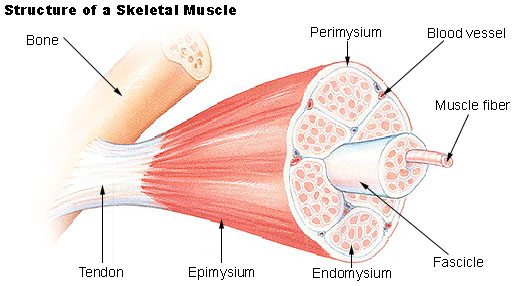
\includegraphics[width=1\linewidth]{./figure/muscle_scaffold.jpg}
    \caption{Connective Tissue Scaffold of Muscle \footnotesize{(Public Domain figure from \href{https://commons.wikimedia.org/wiki/File:Illu_muscle_structure.jpg}{Wikimedia Commons})}}
    \label{fig:muscle_scaffold}
\end{figure}

\subsection{Roles of the Connective Tissue Scaffold}

The endomysium, perimysium, epimysium connective tissue scaffold connect, contain and arrange muscle fibers. There are two other notable functional roles. First, they transmit tension and to and through tendons to attachments \cite{turrina_muscular_2013}. Second, they secure the physical location and approximation of the neurovascular supply to the muscle fibers.

\subsubsection{Transmit Tension}

Each muscle fiber transmits tension to one another and through the connective tissue scaffold. To transmit tension the connective tissue must securely, and with minimal elasticity, connect each muscle fiber to each other and to the tendon. The endomysium and perimysium tend to be thinner and contain both collagen and reticular fibers. Whereas the epimysium tends to have a greater volume of collagen (less elastic). 

The transmission of tension from muscle fiber to tendon to bone includes two zones of transition: muscle-to-tendon, and tendon-to-bone. The muscle-to-tendon zone is referred to as the \textbf{musculotendonous junction (MTJ)}. The MTJ is where muscle fibers start to diminish and muscle connective tissue, primarily epimysium starts to increase and meet the collagenous tendon tissue. From the muscle fibers toward the tendon the MTJ includes multi directional tendon projections gradually reorienting to being longitudinally oriented tendon tissue which allows a uniform transmission of tension. The multidirectional projections combine the muscle fiber tension to the tendon \cite{knudsen_human_2015}. Tendons consist of dense connective tissue that allows them to absorb and transmit substantial tension. Tenocytes (cells that make tendons) account for about 20\% of tendon volume, and the extracellular matrix (ECM) accounts for about 80\% of tendon volume \cite{kjaer_role_2004}. 

The tendon-to-bone zone is referred to as the tendon-bone attachment. The formation of an attachment between tendon and bone starts during embryonic development. During musculoskeletal system assembly, the tendon–bone attachment  forms a structure that is mechanically complex given the need to transfer tension between two materials that differ greatly in stiffness (tendon being non mineralized connective tissue, and bone being mineralized connective tissue).    

\subsubsection{Secure the Neurovascular Supply}
The connective tissue scaffold secures the neurovascular supply to muscle to make sure that the neurovascular supply stays were it is supposed to stay. Entering through epimysium and perimysium connective tissue the neurovascular structures (nerves, arteries, veins) are secure in their path regardless of muscle length. They are then embedded in the endomysium in close proximity to the muscle fiber regardless of the length of the muscle. The vascular supply is delivered by arteries and arterioles, and removed by veins and venules. They provide blood flow that penetrates the epimysium and perimysium to reach the muscle fibers. Capillaries then surround each muscle fiber embedded and anchored in the endomysium to interact and exchange mass with the extra-cellular fluid surrounding the sarcolemma. Innervation of muscle for both excitation (Chapter \ref{chp:excitation} and regulation (Chapter \ref{chp:regulation}) by the nervous system comes from branches of peripheral nerves that penetrate the epimysium and perimysium and terminate in and are anchored by the endomysium at the required location for each muscle fiber (at the neuromuscular end plate).


\section{Muscle Mechanics}

Chapter 2 on Tension focuses on the mechanisms internal to a muscle fiber for generating tension. Our inclusion of muscle fiber mechanics here is a first pass on basic topics of muscle mechanics such as passive and active tension, pennation, and the velocity of changes in length ($\Delta$ length).

% Left off second draft editing here on May 30

\subsection{Active \& Passive Tension}

Tension created by a muscle fiber is active or passive. Active tension is created when the muscle fiber is activated via excitation of its membrane which triggers processes that transform chemical into mechanical energy. Activation as a word captures the essence of active tension and is preferred to the more commonly utilized term, contraction. The mechanical energy of activation pulls the ends of a muscle fiber together. It attempts to shorten the muscle fiber and through transmission of that tension to the connective tissue scaffold it attempts to shorten the entire muscle (bring the tendon attachments together). Passive tension is generated when an "other force" lengthens the muscle and its fibers. This "other force" is always external to the muscle fiber (or muscle) itself. The other force can be another muscle, or it can be external to the musculoskeltal system completely, such as gravity. Passive tension occurs when an external force attempts lengthen the muscle fiber. For a muscle \textit{in situ} this is commonly when an external force pulls the tendon attachments apart, and in response the muscle and its fibers create tension that resists lengthening \textbf{without} activation. 

\subsection{Pennation - Fascicle Arrangement}

Fascicles can be organized (mostly) parallel to the overall tendon line of pull, or with an angle between the fascicle and the overall tendon line of pull. Figure \ref{fig:pennation} shows an arbitrary muscle with a line of pull of the whole muscle along the overall tendon line in red (force of the whole muscle ($F_{wm}$)); and the line of pull of the muscle fibers bundled in fascicles at angle $\alpha$ in orange (force of the fiber ($F_{fiber}$)). When there is an angle, such as $\alpha$, the muscle is pennnated. Pennation exists when there is an angle between the line of pull of the fascicles and the line of pull of the tendons. In Figure \ref{fig:pennation} the line of pull of the tendon is the vector sum of the lines of pull of the fascicles. With pennation there is a vector component of the muscle fiber that acts in line with the tendon pull, and there is a vector component that does not work in line with the tendon pull. The vectors that act in line with the tendon pull sum together; whereas the vectors that do not act in line of the tendon pull cancel each other out. Fascicle arrangement is one of the primary features that distinguishes various classifications of muscles.

\begin{figure}[!ht]
    \centering
    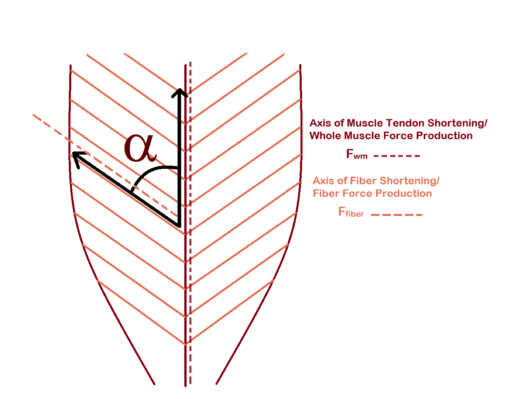
\includegraphics[width=1\linewidth]{./figure/pennation.png}
    \caption{Pennation of Muscle Fibers \footnotesize{(Public Domain figure from \href{https://commons.wikimedia.org/wiki/File:Pennation_angle_of_fibers_in_pennate_muscle.png}{Wikimedia Commons})}}
    \label{fig:pennation}
\end{figure}

Fascicle arrangement is a muscle \textit{in situ} factor that influences the velocity of shortening of the muscle per unit of shortening of a muscle fiber; and the force of activation. For the most part fascicle arrangement is not a modifiable aspect of a muscle. There are no training (stretching, pulling, needling, strengthening) programs that alter a particular muscles pennation status (such as whether it is pennated or not). However, there is evidence of particular types of training having a small influence on the angle of pennation \cite{cuthbert_effect_2020}.

\subsubsection{Velocity of Shortening}
 
If two muscles, one pennated and one not pennated, had a set of homogeneous muscle fibers that all shortened at the same velocity during activation with no resistance; the muscle without pennation would shorten with a higher velocity. This occurs because the shortening of each fiber is summed to the whole muscle. If each fiber shortens to 50\% of its length in one second, then the muscle as a whole would shorten to 50\% of its length in one second. However, in a pennated muscle, when each fiber shortens to 50\% of its length in one second, the muscle as a whole shortens at about 50\% $\times \cosine(\alpha)$ (recall that $\alpha =$ angle of pennation). For example, if $\alpha = 35^\circ$ then with all muscle fibers shortening 50\% in 1 second there would be about 40\% in 1 second.

\subsubsection{Force of Active Tension}

The amount of force that a muscle can develop during maximal activation is proportional to the cross sectional area (CSA) of the muscle. The force of the whole muscle is proportional to the number of parallel muscle fibers that are activated. Note the stipulation that these fibers must be parallel. Adding muscle fibers in series (which make a muscle longer but not thicker) does not contribute to the force generated by the entire muscle (at its ends). In series each muscle fiber pulls from both ends during activation and some of the force is cancelled out. In Figure \ref{fig:Sacromeres_series_parrallel} there are three fibers in series (A) and in three fibers in parallel (B). In series the forces from 1 and 2 cancel each other out and the force of 3 is transmitted to the the ends. When in parallel the forces of the three sum. Note that the muscle fibers in parallel increase the CSA.

\begin{figure}[!ht]
    \centering
    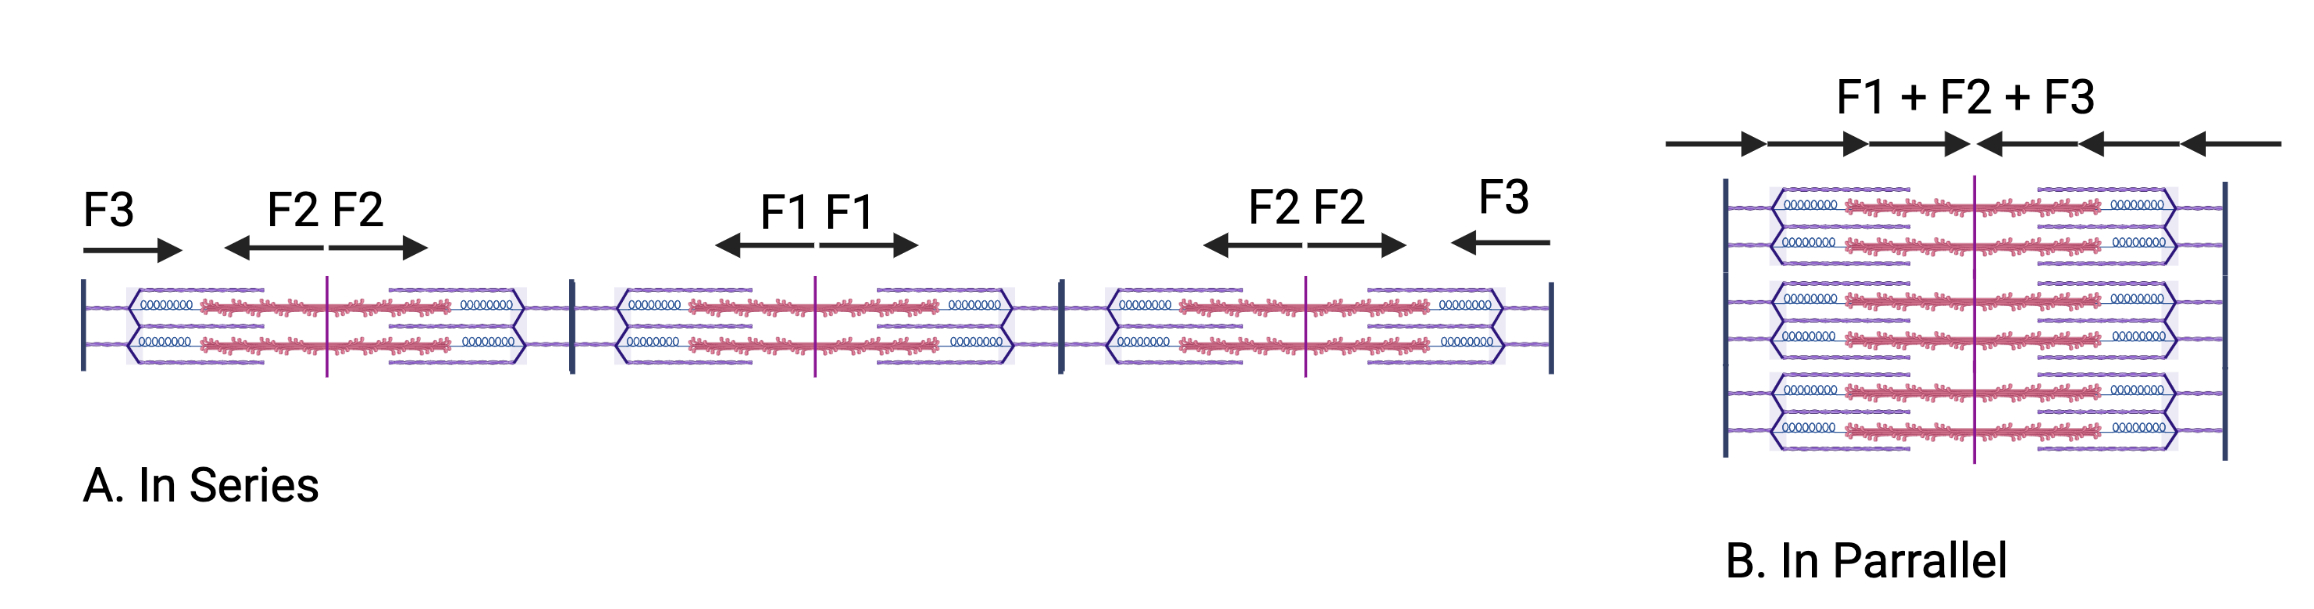
\includegraphics[width=1\linewidth]{./figure/Sarcomeres_series_parrallel.png}
    \caption{Muscle Fibers in Series \& Parallel \footnotesize{(Created with Biorender.com)}}
    \label{fig:Sacromeres_series_parrallel}
\end{figure}


Pennation tends to increase the CSA (the number of muscle fibers in parallel). Similar to the loss of velocity in a pennated muscles, not all of the muscle fiber tension is transmitted to the line of pull of the tendon and thus is lost. However, the increase in CSA compensates for loss in force associated with the vector sum. For example, if a muscle fiber can generate 1 unit of force and we have 50 fibers in parallel the muscle as a whole can generate 50 units of force. If we can get 100 fibers in parallel with a pennated arrangement of those fibers with an angle of pull that transmits 70\% of the force to the line of pull of the tendon then the muscle can generate 70 units of force. Despite a slight loss of efficiency at the level of the muscle fiber (less tension transmits to the line of pull of the tendon), there is a gain in tension at the level of the muscle. Muscles that are not pennated (fusiform or strap muscles) tend to have higher velocities of shortening during unresisted active tension and lower maximal forces during resisted active tension.

\subsubsection{Overall Effect of Pennation}
Pennation tends to be a decrease in velocity of shortening during unresisted activation and an increase in maximal force during resisted activation. These variations (pennation or not pennation) do not occur due to muscle adaptations to training or other modalities. There is some evidence that angles of pennation can be modified slightly, and there is evidence that all muscles can change their cross sectional area regardless of their pennation status. 

\subsection{$\Delta$ Length During Activation}

$\Delta$ length is a change in length of a muscle. By convention, negative $\Delta$ length indicates a muscle shortens, positive $\Delta$ length indicates a muscle is lengthening and zero $\Delta$ length indicates a muscle does not change length. Activation types are defined based on the $\Delta$ length during activation.\footnotemark\footnotetext{You my have learned these as contraction types. You should be comfortable exchanging the terminology muscle contraction for muscle activation and vice versa. However, activation is the preferred language for this course and avoids some of the confusion with eccentric activation.} 

\begin{table}[h!]
\centering
\begin{tabular}{||c c c ||} 
 \hline
 $\Delta$ Length & Muscle & Activation Type \\ [0.5ex] 
 \hline\hline
 Negative & Shortens & Concentric \\
 Zero & Does not change & Isometric \\[1ex] 
 Positive & Lengthens & Eccentric \\[1ex] 
 \hline
\end{tabular}
\caption{Classification of $\Delta$ Length During Activation}
\label{table:contraction_types}
\end{table}


Anything other than a concentric activation requires counteracting forces. A muscle not connected to anything and not under the influence of other forces will shorten (negative $\Delta$ length) with activation. To have activation of a muscle with 0 $\Delta$ length (isometric) or positive $\Delta$ length (eccentric) requires other forces such as other muscles or external forces acting on the joint(s). Forces acting on joints create joint movement based on the torque being created. Therefore, whether a muscle has a concentric, isometric or eccentric activation depends on the balance between torque it is creating (muscular or internal torque) and the torque being created by all other forces acting at the joint. If the forces are coming from outside of the body then they are called external torque. 

\vspace{0.2cm} 
The free body diagram in Figure \ref{fig:int_ext_torque} shows the biceps muscle acting as an elbow flexor in two situations. In  \ref{fig:int_ext_torque}-A the internal force of the biceps muscle is creating \textbf{MORE} flexion torque than the external force is creating extension torque. Therefore the elbow flexes. Since the biceps muscle fibers are activated with a negative $\delta$ length it is a concentric activation. Since it is creating flexion, it can be called concentric flexion. In  \ref{fig:int_ext_torque}-B the internal force of the biceps muscle is creating \textbf{LESS} flexion torque than the external force is creating extension torque. Therefore the elbow extends. Since the biceps muscle fibers are activated with a positive $\delta$ length it is an eccentric activation. The external force is creating extension and the biceps are resisting extension, it can be called eccentric extension.

\begin{figure}[!ht]
    \centering
    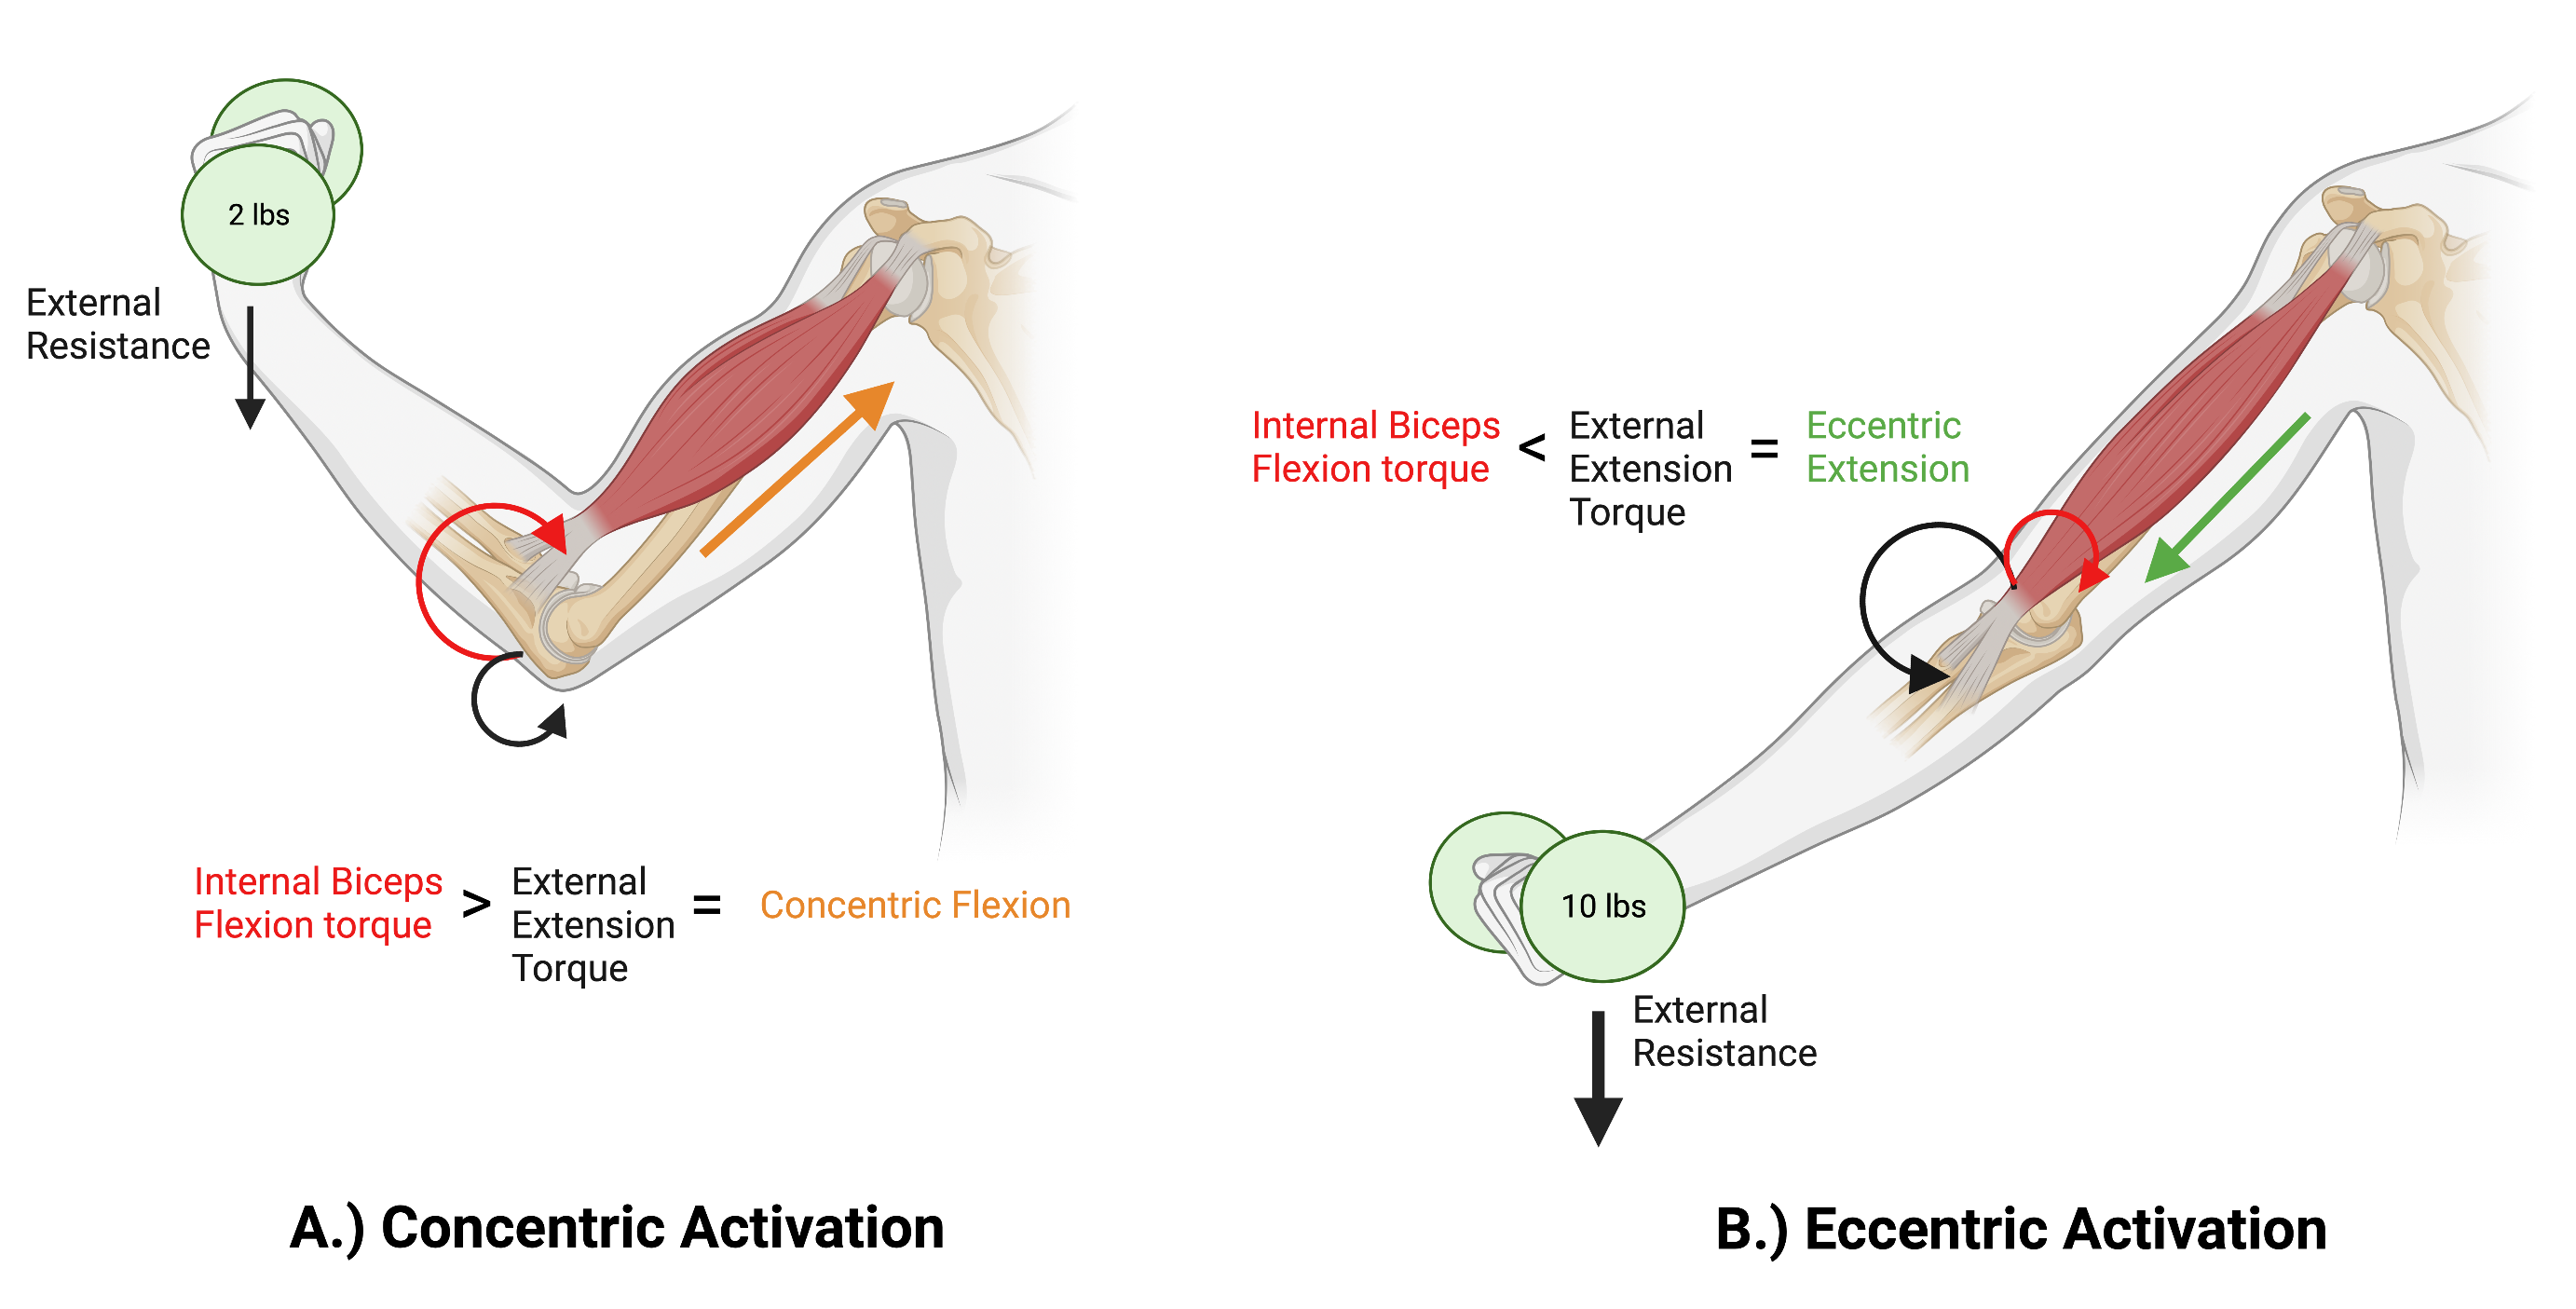
\includegraphics[width=1\linewidth]{./figure/int_ext_torque.png}
    \caption{Biceps Muscle Concentric Flexion vs. Eccentric Extension \\ \footnotesize{(Created with Biorender.com by Ashley Ney, SPT, PSU DPT Class of 2025)}}
    \label{fig:int_ext_torque}
\end{figure}

\vspace{0.2cm} 

The free body diagram in Figure \ref{fig:free_body_diagram} shows the forces and related torque during the nordic hamstring exercise (NHE). During this exercise the subject is on their knees with their ankles supported so that the lower limb (below the knee) cannot move. The subject keeps their hips straight and slowly shifts their body mass forward. Once the body mass (black arrow) is anterior to the axis of rotation of the knee it creates a knee extension torque (black circular arrow). The subject allows themselves to not fall forward to quickly but usually reaches a point where they can no longer slow their descent and they fall to the floor. While they are attempting to slow their descent to the floor they are using their hamstring muscles which create a force through active tension (red arrow), which then creates a knee flexion torque (red circular arrow). The exercise can be done a variety of ways. In one scenario the subject can stop and hold themselves in one position. In another scenario, after holding themselves they can use the force of hamstring active tension to bring them upright again. 

\begin{figure}[!ht]
    \centering
    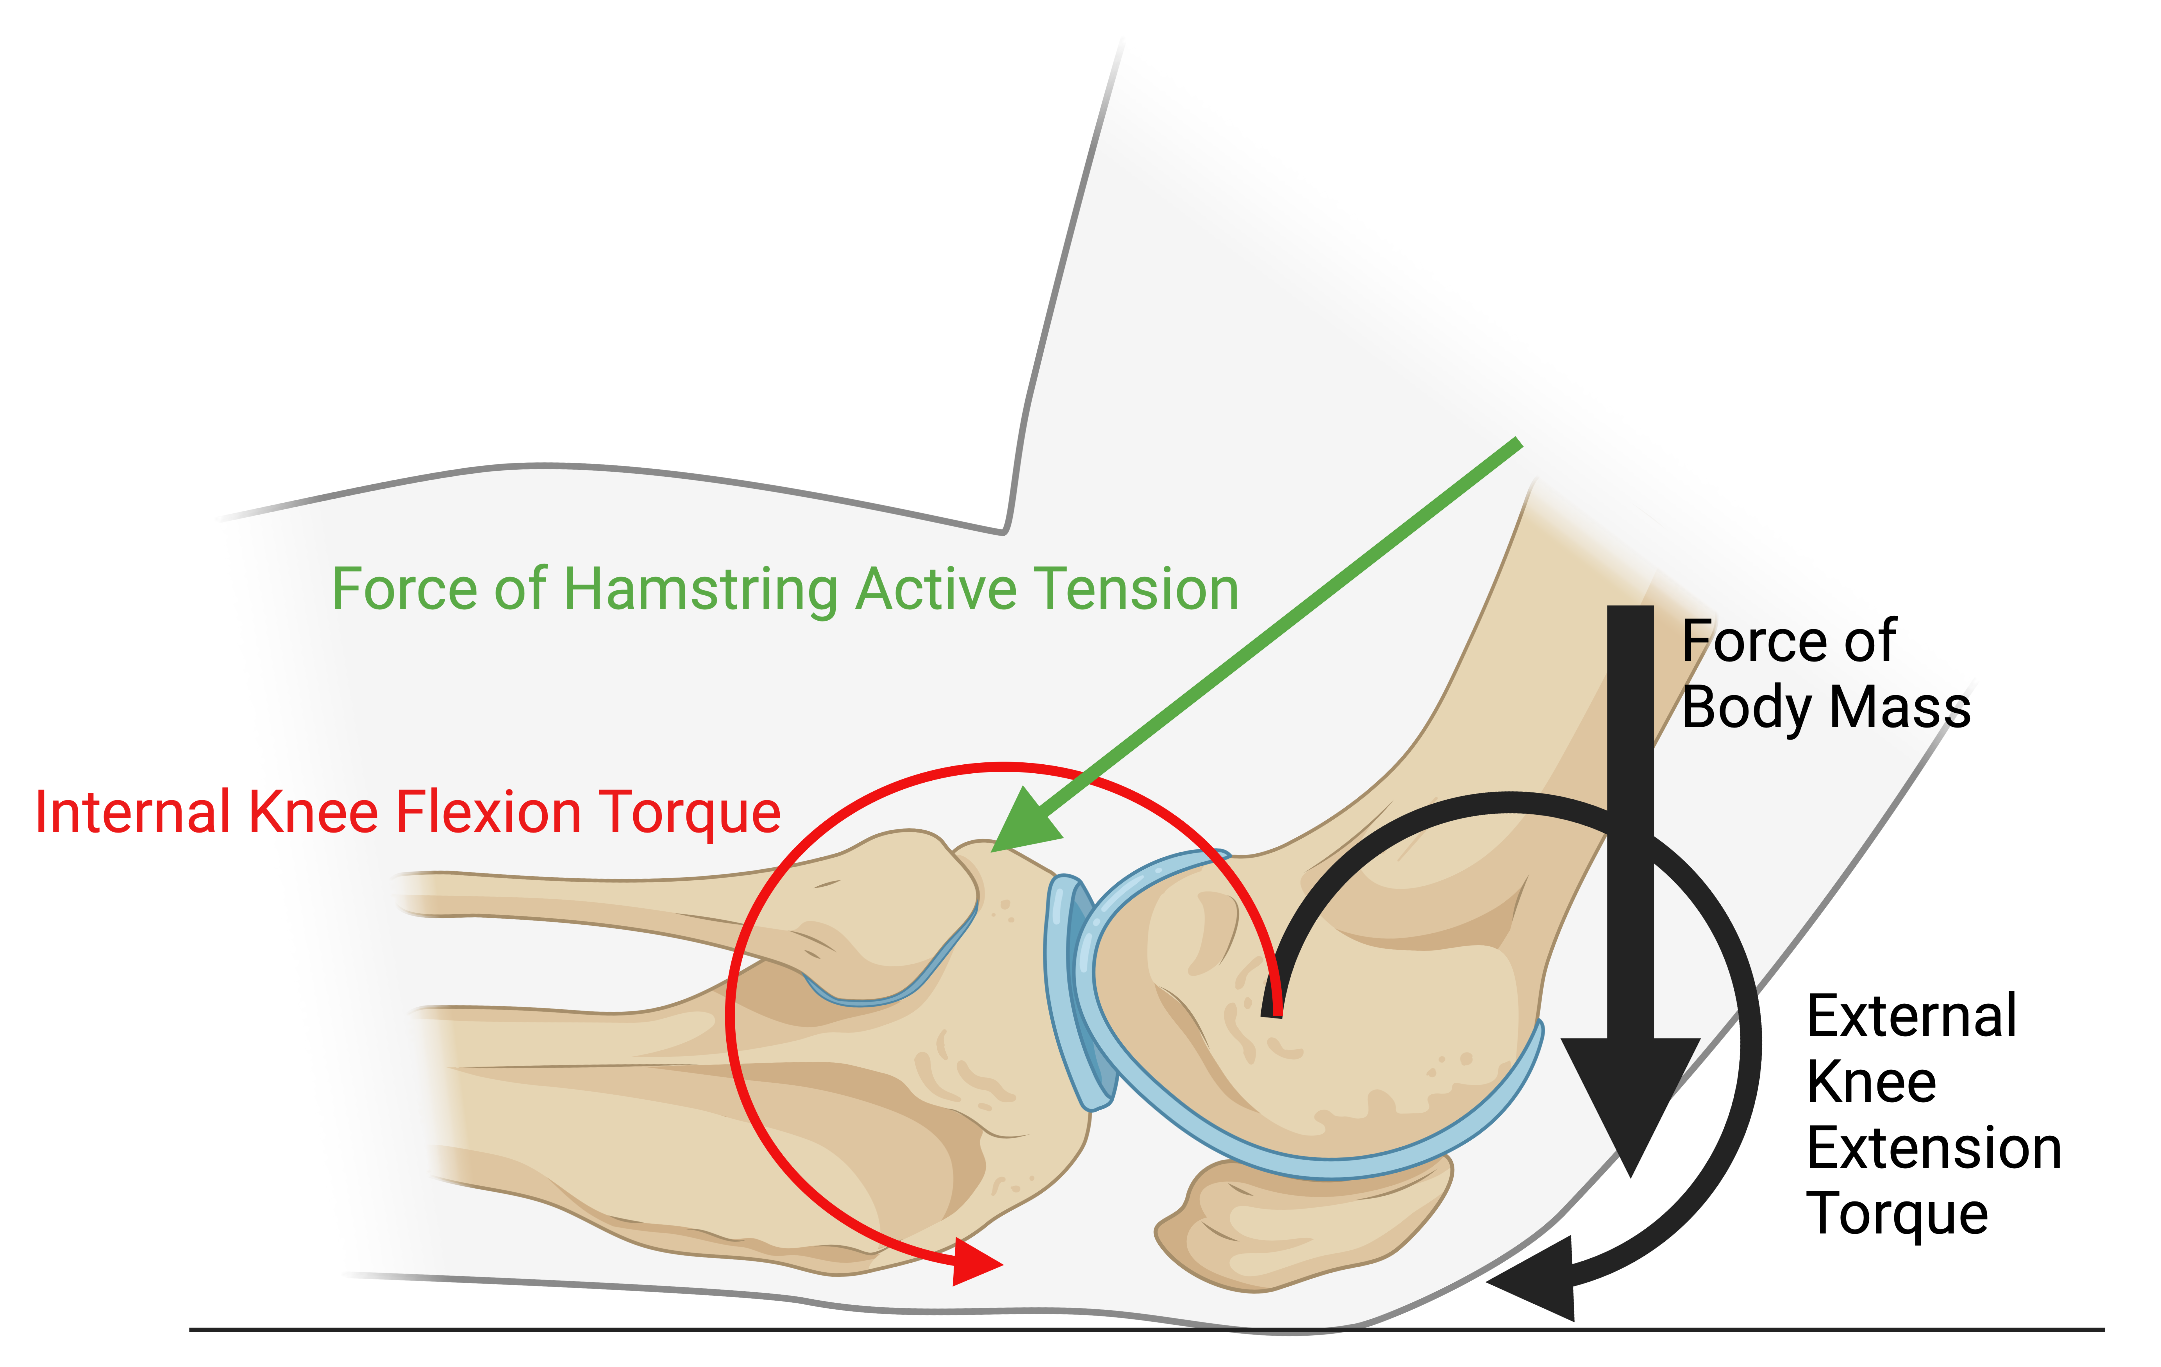
\includegraphics[width=1\linewidth]{./figure/free_body_diagram.png}
    \caption{Free Body Diagram of the Nordic Hamstring Exercise \\ \footnotesize{(Created with Biorender.com by Ashley Ney, SPT, PSU DPT Class of 2025)}}
    \label{fig:free_body_diagram}
\end{figure}

There is a relationship between the force of the body mass ($F_{bm}$) and the knee extension torque created by the body mass ($T_{bm}$) which is external since it is the result of gravity. There is a relationship between the force of the muscle ($F_{m}$) and the knee flexion torque created by the muscle ($T_{m}$), which is an internal or muscular force. The muscular force varies based on how much tension is created by the muscle activation. Movement depends on the relationship between the two opposing torques as seen in Table \ref{table:NHE}. The movement and the activation type are dependent on the relationship of the torques. The torques are related to both the force generated by the tension of the muscle, the body weight and their respective perpendicular distances.\footnotemark{}\footnotetext{This book will not spend much time at this level of analysis. However, if you are not comfortable with torque and vectors from physics and other courses you have had it is a worthwhile to refresh your memory now.}

\begin{table}[h!]
\centering
\begin{tabular}{||c c c c c||} 
 \hline
 Torque Relationship & $\Delta$ Length & Muscle & activation Type & Movement\\ [0.5ex] 
 \hline\hline
$T_m > T_{bm}$ & Negative & Shortens & Concentric & Knee Flexion \\
$T_m = T_{bm}$ & Zero & Does not change & Isometric & No Movement\\[1ex] 
$T_m < T_{bm}$ & Positive & Lengthens & Eccentric & Knee Extension \\[1ex] 
 \hline
\end{tabular}
\caption{$\Delta$ Length During Active Tension Based on Torque Relationships}
\label{table:NHE}
\end{table}

\begin{question}{Questions}
\begin{flushleft}  
If an external flexion torque is less than an internal (muscle tension generated) extension torque, what would be the movement and the type of muscle activation? \\
If an external extension torque is greater than an internal (muscle tension generated) flexion torque, what would be the movement and the type of muscle activation?
\end{flushleft}
\end{question}

\section{Muscle Roles}

\begin{itemize}
\item Agonist: Muscle creating tension for the intention of the movement.
\item Antagonist: Muscle that creates the opposite movement of the agonist.
\item Synergists: Muscles that work together and combine their tension to create a movement. We can talk about synergist agonists and synergist antagonists, though the former is typically the intention when just referring to synergists.
\item Stabilizer: Muscles that provide tension to neutralize certain motions toward the purpose of a movement
\end{itemize}

To define a muscle role we must consider context. Context for muscle roles are typically movements. Movements include all the motions that are occurring, the directions of those motions and the intention of the mover doing the movement. If the movement is the downward phase of a squat one of the motions is knee flexion. The intention of the mover is knee flexion (they intend to move downward). The knee extensor muscles are involved as agonists even though knee is flexing. Just because the motion is knee flexion, the agonists are not necessarily the knee flexors.

\section{Summary}

This chapter covered some of the fundamentals of muscle function. We discussed how the connective tissue scaffold allows muscle fiber tension to transmit to the muscle tendon and bony attachments for the purpose of whole muscle tension, including what it means to consider a muscle \textit{in situ}, and how that same scaffold provides an anchor for the neuromuscular supply and the overall shape of a muscle, including fascicle arrangement. Fascicle arrangement influences how the muscle \textit{in situ} force and length is related to muscle fiber force and $\Delta$ length. Not only a particular muscle’s activation, but other forces, have an integral influence the $\Delta$ length of a muscle during activation and therefore activation type. Finally we classified four muscle roles, agonist, antagonist, synergist and stabilizer. The next chapter covers the muscle fiber, its structure and the mechanisms involved in attaining and sustaining both active and passive tension.

\printbibliography[heading=subbibintoc]

\section*{Sample Questions}

\begin{enumerate}
    \item A muscle in its original position is:
    \item Once tension is attained, how long does a muscle need to sustain tension?
    \item A fascicle is surrounded by?
    \item Two muscles are maximally activated and shorten in one second. Muscle A shortens 75\% of its length. Muscle B shortens to 50\% of its length. Which muscle is more likely to have fascicle pennation?
    \item Delta length is Zero and the muscle is activated. What type of contraction is the muscle undergoing?
    \item If an external flexion torque is greater than an internal (muscle tension generated) extension torque, then what is the joint movement and what type of contraction is occurring?
\end{enumerate} 

%%%%%%%%%%%%%%%%%%%%%part.tex%%%%%%%%%%%%%%%%%%%%%%%%%%%%%%%%%%
% 
% sample part title
%
% Use this file as a template for your own input.
%
%%%%%%%%%%%%%%%%%%%%%%%% Springer %%%%%%%%%%%%%%%%%%%%%%%%%%

\begin{partbacktext}
\part{Muscle Function Overview}
\noindent 
Part II on Muscle Function includes four short chapters directly related to how muscles generate tension. Tension generating mechanisms are the primary focus of Chapter \ref{chp:tension} on Tension. To generate active tension a muscle fiber must be excited - Chapter \ref{chp:excitation} on Excitation introduces the general concepts of an excitable membrane and signaling processes and how these relate to excitation - contraction coupling. Muscle function depends on sequences of excitation, across time and space, that determine the rate and quantity of active muscle tension. Chapter \ref{chp:regulation} on Regulation describes the basic mechanisms of regulation of muscle active tension and tone by the central and peripheral nervous system. With all of that in place, we are ready to turn our attention in Chapter \ref{chp:energetics} on Energetics to the transfer of chemical energy as delivered to the muscle fiber as glucose or fat to mechanical energy in the form of tension. 
\end{partbacktext}
\include{chapter/tension}
\include{chapter/excitation}
\include{chapter/regulation}
\include{chapter/energetics}
%%%%%%%%%%%%%%%%%%%%%part.tex%%%%%%%%%%%%%%%%%%%%%%%%%%%%%%%%%%
% 
% sample part title
%
% Use this file as a template for your own input.
%
%%%%%%%%%%%%%%%%%%%%%%%% Springer %%%%%%%%%%%%%%%%%%%%%%%%%%

\begin{partbacktext}
\part{Muscle Support}
\noindent 
\section*{Muscle Support Overview}

The chapters of Part III are about the supportive environment of the extracellular fluid (ECF). Every chapter describes a set of functions that serve the purpose of delivering, removing or regulating the contents of the ECF. 

Figure \ref{fig:part3_overview} is a graphic overview of the ECF supporting functions. Filtration relies on micro-circulation which relies on circulation. Circulation is the flow of blood through the entire circulatory system. Circulation of blood through the entire body ensures regular mixing of the ECF contents throughout the body. This mixing ensures consistency of ECF contents and a stable environment for all the cells of the body. For example, if blood $Na^+$ concentration is tested, it is properly assumed that concentration is the concentration of $Na^+$ throughout the entire ECF. Circulation also allows each supporting system contribute - either to adding water, heat, ions, molecules or nutrients to the ECF, or removing by-products from the ECF. Supporting systems are also in communication with one another based on the circulating substances and messages (hormones). For example, if a muscle working at high tension is shuttling lactate into the ECF, it is picked up by the circulation and can then enter other cells (heart, liver, non working muscles) where lactate levels are low. In these cells the lactate can be used to produce an $NADH$ from $NAD^+$, and a pyruvate to proceed into the mitochondria. 

\begin{wrapfigure}{R}{0.5\textwidth}
  \begin{center}
   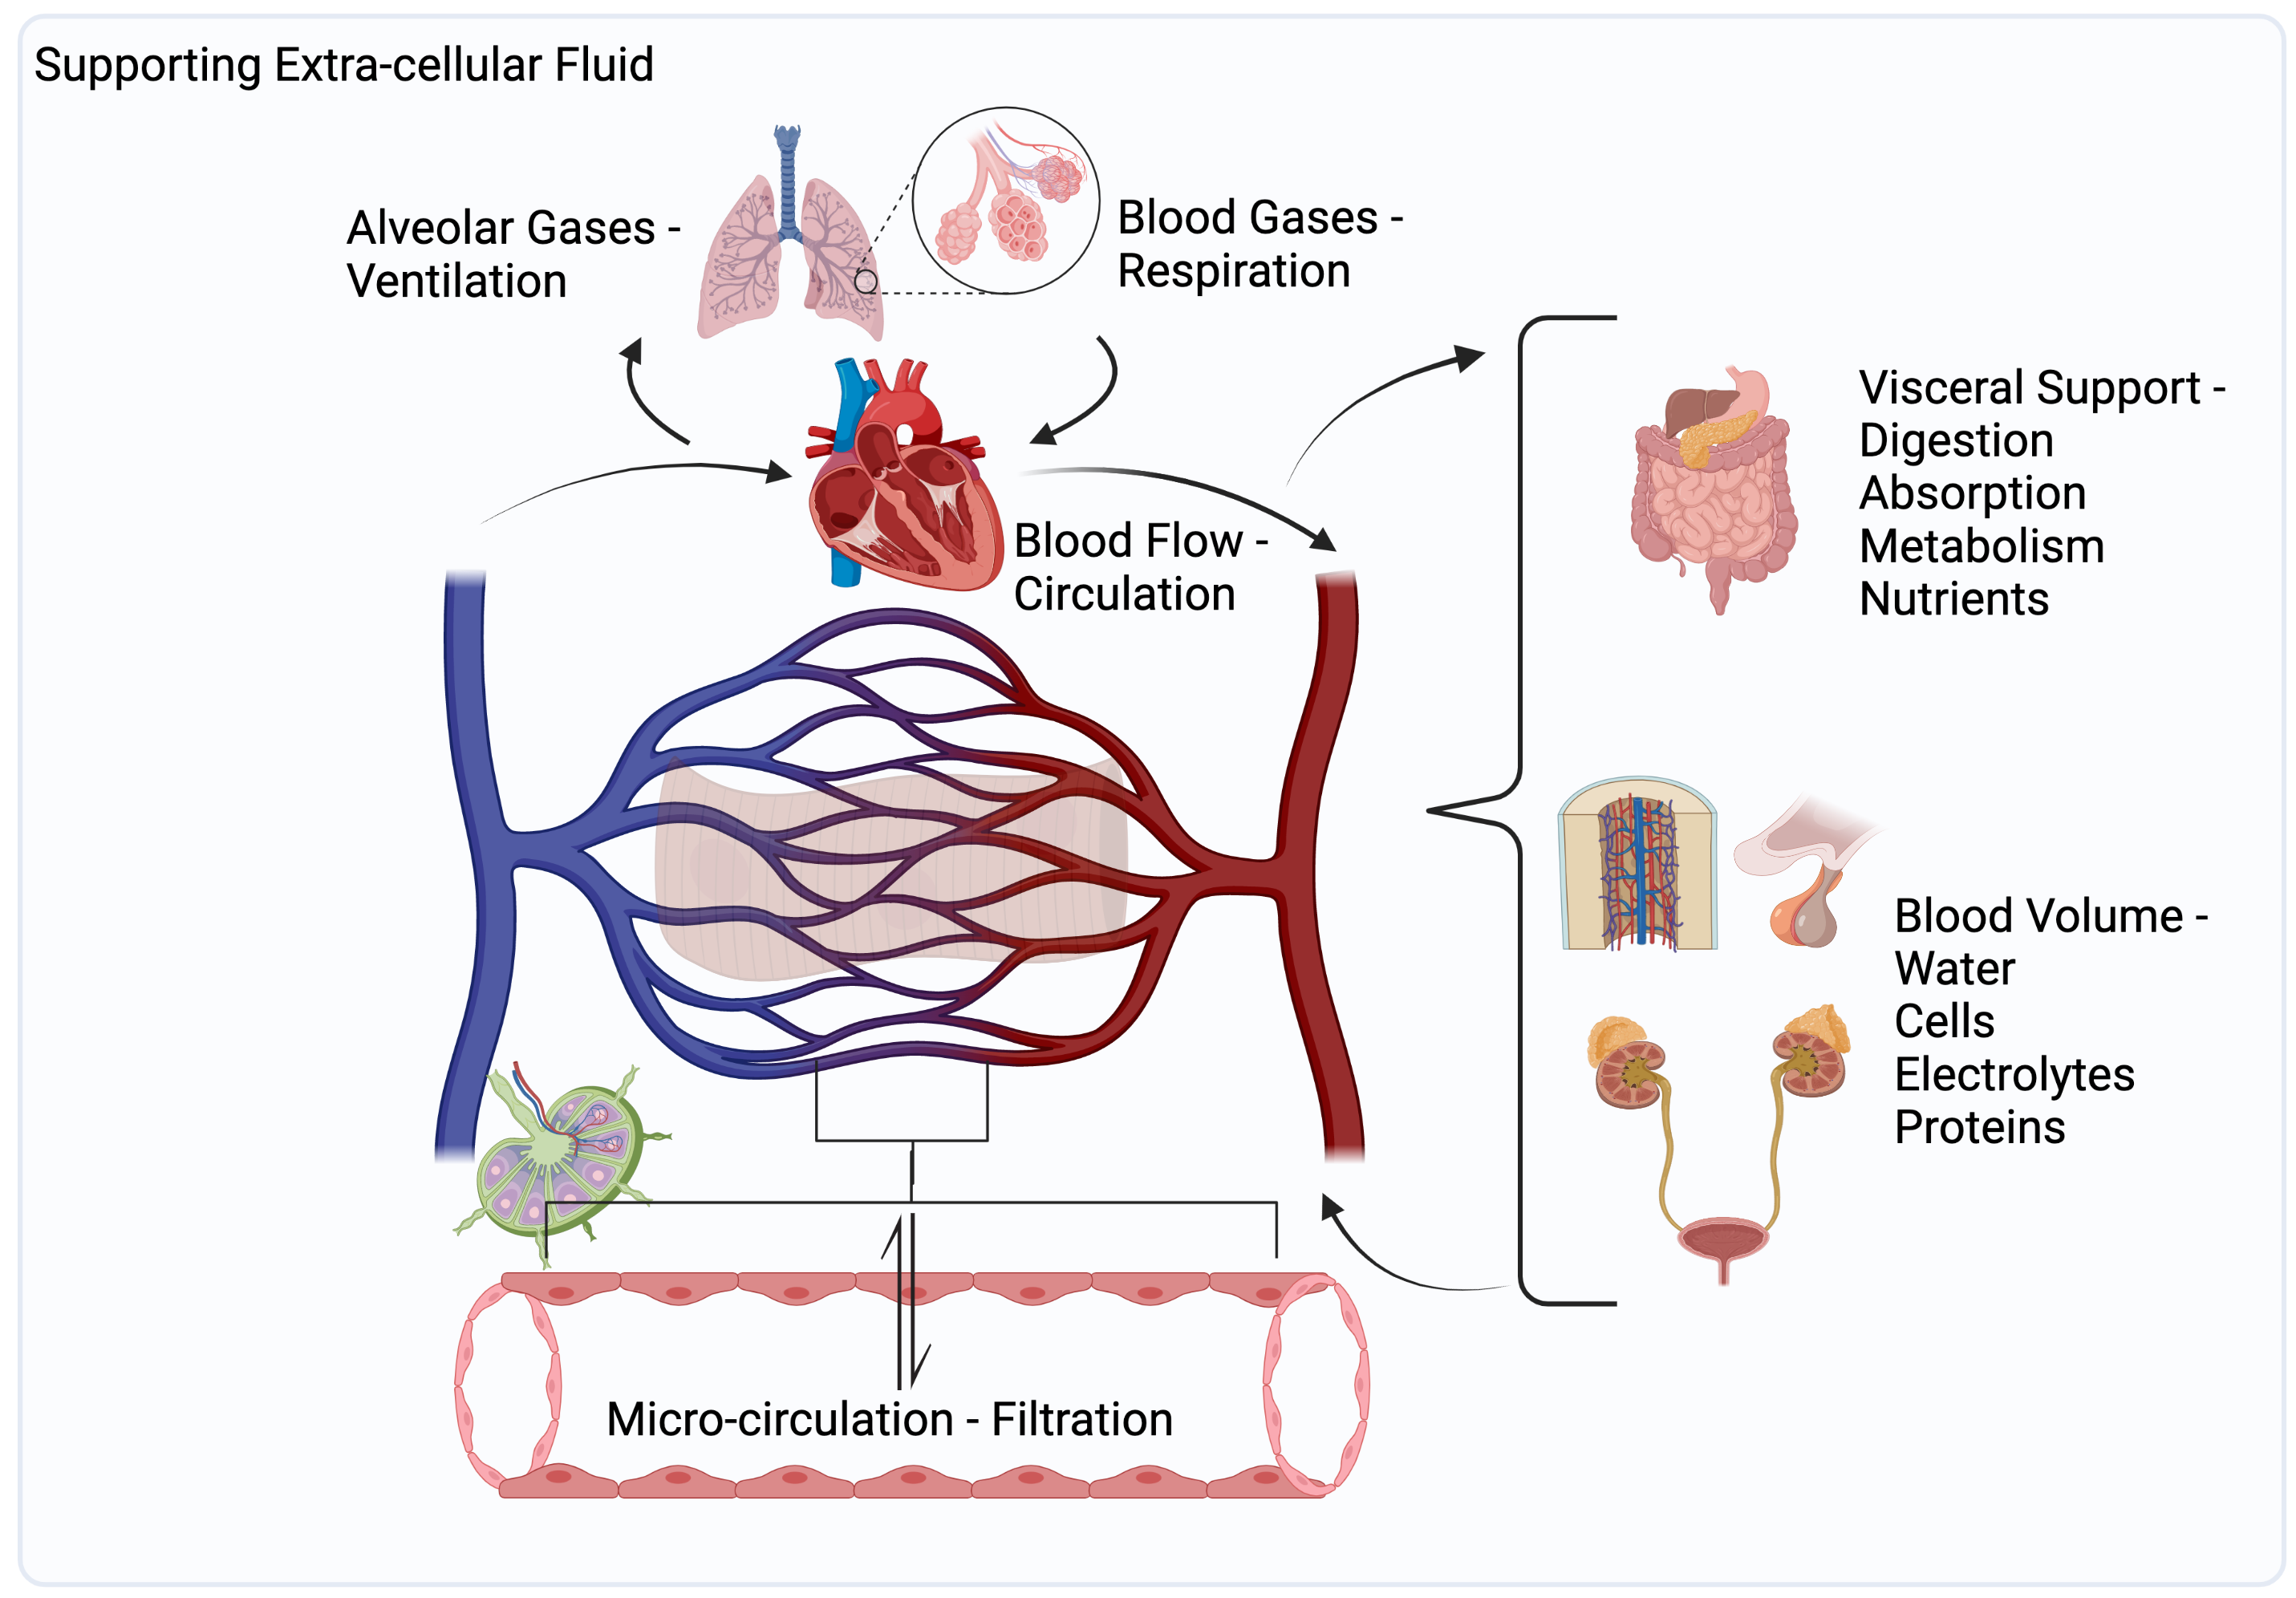
\includegraphics[width=1.0\linewidth]{./figure/part3_overview.png}
  \end{center}
  \caption{Part III: Muscle Support Overview \footnotesize{(Created with BioRender.com)}}
    \label{fig:part3_overview}
\end{wrapfigure}

The contents of blood, and therefore ECF, is regulated and supported by renal filtration (kidneys) and the endocrine system. The regular circulation of blood through the kidneys involves several mechanisms that selectively filter the blood and in doing so regulate the ECF, and therefore the ICF volume. The regulation of fluid volume includes the regulation of several important ions (electrolytes) and the removal of waste (i.e. urea). Working with the endocrine system the kidneys provide long term regulation of blood pressure, which is important for circulation; as well as red blood cells, which is important for oxygen carrying capacity.

Cellular respiration in the mitochondria is constantly using $O_2$ and producing $CO_2$. These molecules are called gases (blood, alveolar) because their natural state is in the gaseous form. The micro circulation ensures the regular delivery ($O_2)$ and removal ($CO_2$) of these gases from the interstitial fluid. The circulation to the lungs ensures the regular exchanges of these gases with the environment. Blood gases rely on blood flow through the lungs for respiration (gas exchange) between the blood and alveoli. Respiration depends on ventilation, the regular movement of these gases into and out of the lungs with the bulk transport of air. 

Maintaining blood nutrients relies on digestion, absorption, metabolism and elimination by the gastrointestinal organs and the liver. Based on the basic physiological concept of mass balance the regular elimination of water requires the regular intake of water. The regular transformation of the carbon bond energy from carbohydrates and fats requires the regular intake of carbohydrates and fat. The regular use, breakdown and elimination of proteins for cellular functions requires the regular intake of protein. 

Together these systems support the ECF and therefore muscle fibers and muscle function. They maintain homeostasis of several important electrolytes (ions, including $H^+$ as measured by pH), nutrients, molecules, water and heat (temperature). The systems are are integrated with several interactions and redundancies to provide support across a wide range of muscle demands in a wide range of circumstances, both good and bad.

One difference between Part II and Part III of the book is that many topics throughout the chapters are in Part III are inherently \textit{Clinical Physiology Connections}. Since the concepts described in Part III are traditional concepts in a clinical physiology course, in many ways these chapters are, in their entirety, clinical physiology connections. As the occasion arises, in pace of \textit{Clinical Physiology Connections} there will be \textit{Muscle Connections}.

\end{partbacktext}
\include{chapter/microcirculation}
\include{chapter/renal_clearance}
% !TEX root = ../notes_template.tex

\chapter{Circulation}\label{chp:circulation}
Updated on \today
\minitoc

% Add a section about threats to blood flow such as coagulation gone wrong - too high and too low

This chapter covers the circulation support of micro-circulation, which supports the ECF, which supports skeletal muscle function. Circulation includes two vascular circuits that circulates blood through the systemic and pulmonary circulation. The cardiac pump that supports circulation is covered in the next chapter.  

The primary goal of this chapter is an understanding of circulation in its supportive role for skeletal muscle. Circulation is critical for sustaining the micro-circulation of the ECF for cellular functions throughout the body. Without circulation cells with a high resting metabolism such as the brain and heart can only survive for minutes. The lack of $O_2$ delivery, and lack of $CO_2$ removal being the first two problems that threaten cell life. Problems with circulation can limit the metabolic function of muscles.   

The importance of circulation for life and function makes it a highly studied area of physiology. Since it has been highly studied it has several useful models for understanding circulation. After reviewing the important structures for circulation the chapter introduces several of the useful models (in the form of equations that demonstrate relationships).


\vspace{5mm}
\begin{svgraybox}
\textbf{Objectives include:}
\begin{enumerate}
    \item Describe how the anatomy of the heart and blood vessels supports circulation. 
    \item Identify cardiac anatomy structures.
    \item Explain and Interpret models (equations) of cardiac output, blood pressure and resistance.
    \item Apply equations of cardiac output, blood pressure and resistance (including Poiseuille's Law) to explain and evaluate the function and possible dysfunction of circulation.
    \item Explain circulation regulation based on blood pressure regulation.
    \item Explain circulation distribution and cardiac index.
    \item Explain blood pressure regulation.
    \item Interpret the events of vasovagal syncope.
    \item Perform and interpret cardiovascular tests and measures including: Heart rate and Blood pressure
\end{enumerate}
\end{svgraybox}

\section{Structures of Circulation}

The heart and the roots of the great vessels occupy the pericardium, which is located in the mediastinum. The sternum, the costal cartilages, and the medial ends of the third to fifth ribs on the left side of the thorax create the anterior border of the mediastinum. It is bordered inferiorly by the diaphragm, posteriorly by the vertebral column and ribs, and laterally by the pleural cavity (contains lungs). Specific cardiac structures and vessels are depicted in Figure \ref{fig:Cardiac_Anatomy}.

\begin{figure}[!h]
    \centering
    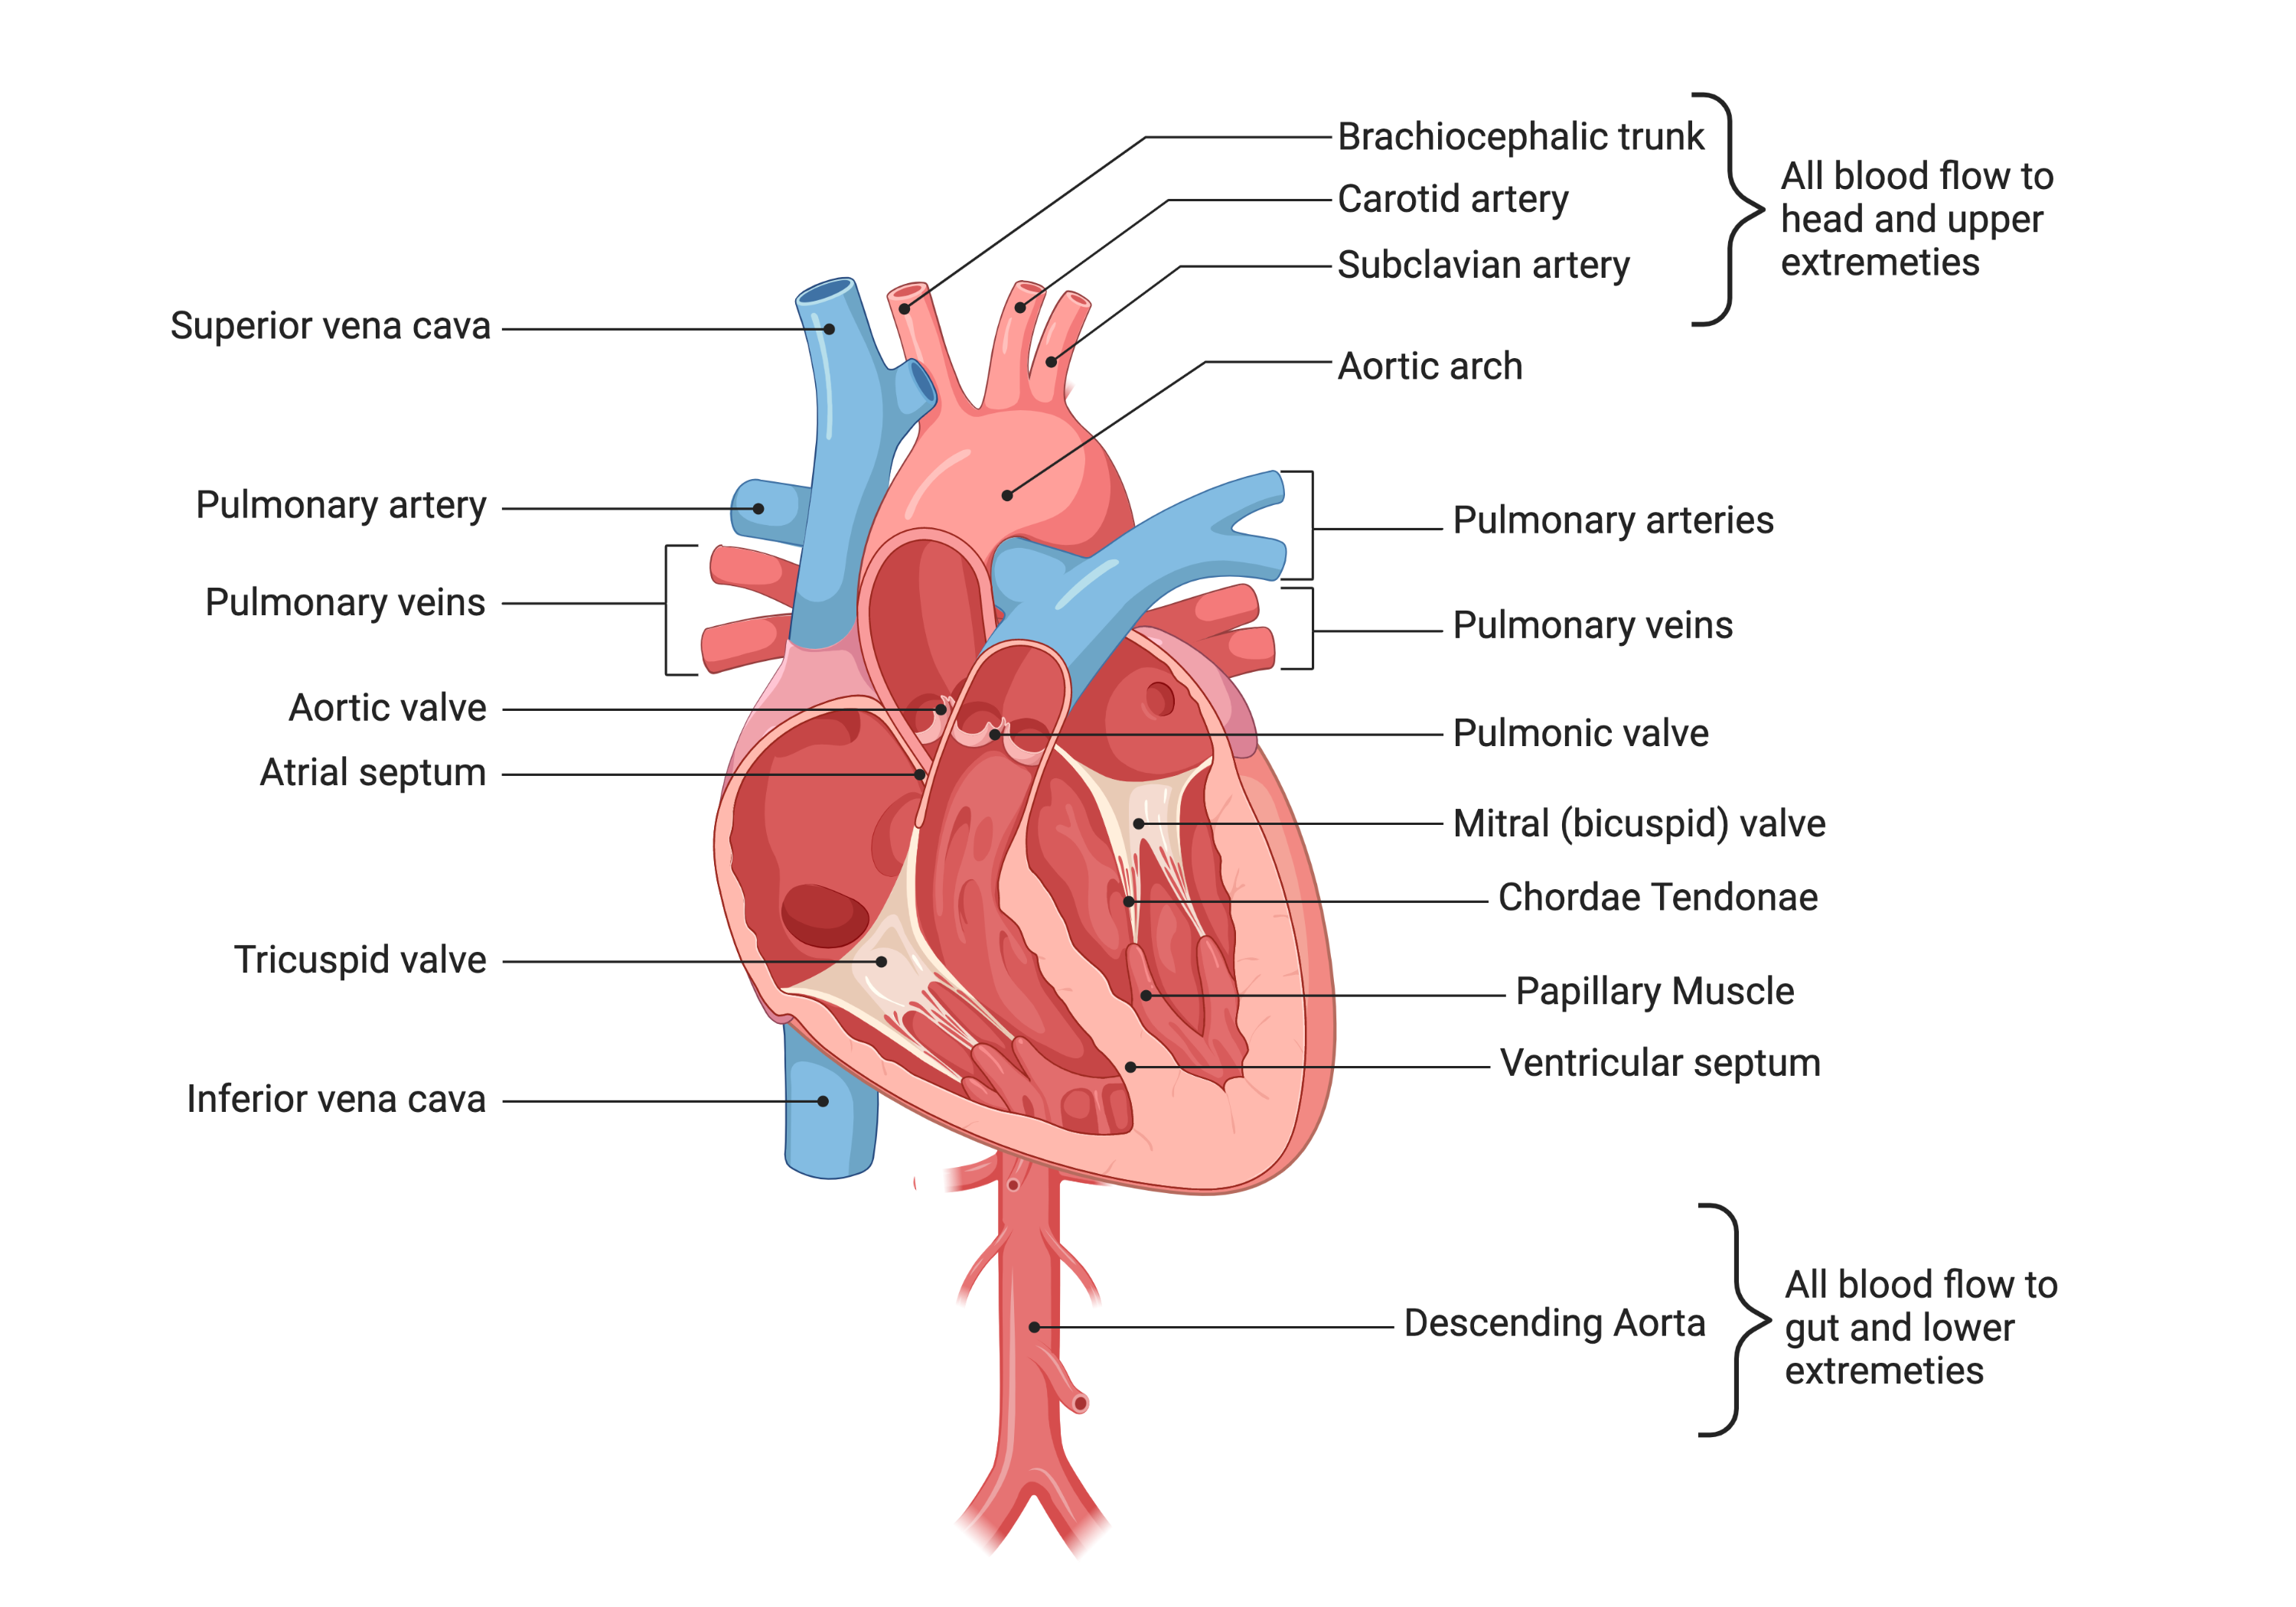
\includegraphics[width=1\linewidth]{./figure/Cardiac_Anatomy.png}
    \caption{Cardiac Anatomy \footnotesize{(Created with BioRender.com)}}
    \label{fig:Cardiac_Anatomy}
\end{figure}

Beyond being familiar with the structure in Figure \ref{fig:Cardiac_Anatomy} that are utilized throughout the chapter, there are several important structural takeaways.

\begin{itemize}
    \item Structurally there are four chambers, right and left atria (RA and LA); right and left ventricle (RV and LV) (the anatomical view).
    \item The four chambers form two primer-pumps for two circulations (right and left), RA and RV for the pulmonary circulation; and LA and LV for the systemic circulation (which includes all skeletal muscles and the heart itself) (the pump view).
    \item Cardiac muscle (myocardium) is thicker in the ventricles than the atria; and on the left side than the right side.
    \item The four chambers are divided into two excitation regions, RA and LA for atrial excitation; and RV and LV for ventricular excitation (the excitation view).
    \item The amount of tension and excitation is related to the thickness of the myocardium; which is based on how much pressure that chamber must generate for circulation.
    \item Circulation between the right and left primer-pumps is prevented by a septum (septal wall), also myocardium, that is thinner than the outer myocardial wall; and also thicker in the ventricles than the atria.
    \item Circulation direction is guided by four one-way valves. Circulation occurs due to pressure gradients - there is nothing inherently directional about pressure gradients other than high pressure to low pressure - therefore the valves are necessary to keep blood flowing from a chamber to the next chamber and now "backwards".
    \item All circulation from the gut and lower extremity passes through the descending aorta; and comes to the heart through the inferior vena cava.
    \item All circulation from the upper extremities and head passes through the great vessels (first three branches off of the aorta); and comes to the heart from the superior vena cava.
    \item For blood to flow through the circulation, venous pressure must be lower than arterial pressure
    \item Venous pressure (systemic in the RA; pulmonary in the LA) refers to the pressure that is the final end point for all venous circulation returning to the heart which must, for circulation to occur, have the lowest venous blood pressure of the respective circulations ($P_{RA} = 0$ when the RA is not generating tension). \item Ventricular systolic pressure refers to the pressure in the ventricles during active tensioning (contraction), for circulation to occur it must have the highest arterial pressure of the respective circulations. The right sided ventricular systolic pressure is lower than the left sided ventricular systolic pressure, the respective circulations are considered low and high pressure.
    \item Because the ventricular systolic pressures must be the highest through the circulation, the tricuspid valve (between the RA and RV) and the bicuspid (mitral) valve (between the LA and LV) have additional support supplied by the papillary muscles and chordae tendonae (the support does not help them open, it prevents them from allowing backflow while closed).
    \item Because the LV has greater pressure than the RR, the mitral valve papillary muscle and chordae tendonae are more developed
    \item The aortic valve, which is not supported by papillary muscle, is under more pressure than the tricuspid valve because the aortic pressure is the second highest pressure in the circulation, however aortic peak pressure is short lived because of how rapidly blood flows out of the aorta.
\end{itemize}

\section{Cardiac Output}

Circulation is measured and assessed based on the cardiac output ($\dot{Q}$) in liters (or mL) per minute. $\dot{Q}$ is the flow of blood through the circuit, hence the circulation. $\dot{Q}$ is directly proportional to the overall pressure gradient and inversely proportional to resistance to circulation. A conceptual understanding of circulation based on ($\dot{Q}$) and the major determinants of, and factors influencing ($\dot{Q}$) facilitates an understanding of both normal and abnormal circulation.

\begin{equation}
    \dot{Q} = \frac{P_{a} - P_{RA}}{TPR}
    \label{eq:Q}
\end{equation}

In Equation \ref{eq:Q}:
\begin{itemize}
    \item $P_{a}$ is pressure in the arteries (arterial pressure, which is highest in the aorta)
    \item $P_{RA}$ is central venous pressure, commonly taken as the pressure in the right atrium (RA)
    \item $TPR$ is the total peripheral resistance of the vascular circuit
\end{itemize}

Equation \ref{eq:Q} is based on Ohm's Law and points attention to the influence of the driving forces for flow (the pressure gradient) and the resistance to flow. Based on the equation it is clear that the pressure gradient is directly proportional to flow (numerator); and resistance is inversely proportional to flow (denominator).

$P_{RA}$ normally approximates to 0. $P_{a} - P_{RA}$ is equivalent to the term $\Delta P$ (change in pressure, pressure gradient) and when $P_{RA} = 0$, then $Delta P = P_{a}$.
However, in various clinical scenarios $P_{RA}$ does not approximate to 0 so it is useful to keep central venous pressure in mind. If there is an increase in $P_{RA}$, without a rise in $P_{a}$ or a drop in $TPR$ then $\dot{Q}$ would be reduced. 

\vspace{.5cm}
An equation that represents the cardiac pump viewpoint of ($\dot{Q}$) is:

\begin{equation}
    \dot{Q} = HR \times SV
    \label{eq:Q_HRSV}
\end{equation}

In Equation \ref{eq:Q_HRSV}:
\begin{itemize}
    \item $HR$ is heart rate in beats per minute (bpm)
    \item $SV$ is stroke volume (the amount of blood pumped during systole) in mL
\end{itemize}

Equation \ref{eq:Q_HRSV} is also easier to confirm, by unit analysis, that these values equate to cardiac output $\dot{Q}$ in mL/min.

\vspace{.5cm}
Combining Equations \ref{eq:Q} \& \ref{eq:Q_HRSV} results in:

\begin{equation}
    HR \times SV = \frac{P_{a} - P_{RA}}{TPR}
    \label{eq:complete_Q}
\end{equation}

The left side of Equation \ref{eq:complete_Q} is based on the output of the heart (cardiac) and the right side is based on the pressure gradient generated by the closed vascular circuit and the resistance encountered by the circulating blood.
To keep the two sides of Equation \ref{eq:complete_Q} equal (balanced) an increase in $HR$ must be balanced with resultant changes in at least one of the other parameters. 

\begin{question}{Conceptual Understanding}
What changes could occur if $HR$ increases to keep Equation \ref{eq:complete_Q} balanced?
What changes could occur if $TPR$ decreased to keep Equation \ref{eq:complete_Q} balanced?
\end{question}

Equation \ref{eq:complete_Q} is a model and is useful to a point. A challenge with this equation, really all of the equations used in physiology, is that the variables are not independent of one another. They are useful for reasoning about the concepts, but not in an exhaustive way. For example, you may have just figured out that to keep Equation \ref{eq:complete_Q} balanced when $HR$ increases, $P_a$ could increase. It turns out that $P_a$ is not independent of $HR$. If $HR$ increases then $P_a$ does tend to increase based on the relationship between arterial pressure and cardiac output.

\subsection{Arterial Pressure ($P_{a}$)}

Equation \ref{eq:Q} simplified under the condition of $P_{RA} = 0$ can be manipulated to provide an equation for arterial pressure:

\begin{equation}
    P_{a} = \dot{Q} \times TPR
    \label{eq:BP}
\end{equation}

Arterial pressure is blood pressure ($P_a = BP$). Equation \ref{eq:BP} shows that blood pressure is directly proportional to cardiac output and total peripheral resistance ($TPR$). It is hoped that seeing the centrality of blood pressure in the equations for $\dot{Q}$ will inspire future clinicians to respect the potency and value of $BP$ measurement in clinical practice. All measured changes in blood pressure (arterial pressure, $P_a$) can be inferred to represent changes in either cardiac output, or total peripheral resistance, or some combination.

Since the heart has two phases - a filling phase known as diastole, and a pumping phase known as systole - it creates pulsatile flow. Systole occurs when the $SV$ is being ejected from the heart. Pulsatile flow creates a rhythmic pulse in $BP$ with a peak value referred to as systolic $BP$ (SBP) and a low value referred to as diastolic $BP$ (DBP). It is useful to consider SBP and DBP separately, as well the mean arterial pressure (MAP):

\paragraph{Mean Arterial Pressure}

\begin{equation}
    MAP = DBP + \frac{1}{3} \times (SBP - DBP)
    \label{eq:MAP}
\end{equation}

MAP is a weighted average blood pressure (average arterial pressure) based on the measured values SBP and DBP. DBP has a stronger influence on MAP than SBP because the time period that circulation is in systole is much shorter than the time they are in diastole. With an increase in heart rate ($HR$) the time in systole becomes proportionally more time but the systolic time interval is relatively unchanged. The change in overall time in systole is based on there being less time in diastole. Despite this there is no modification to the equation for MAP during periods of higher $HR$.

\paragraph{Pulse Pressure}

Pulse pressure (PP) is often considered clinically as the driving pressure for blood flow. PP is calculated as the difference between SBP and DBP ($PP = SBP - DBP$). 

Therefore Equation \ref{eq:MAP} for MAP, can be simplified to:

\begin{equation}
    MAP = DBP + \frac{1}{3} \times PP
    \label{eq:MAP_simplified}
\end{equation}

\subsection{Poiseuille's Law}

Poiseuille's Law offers deeper insight into $\dot{Q}$ and Equation \ref{eq:Q}. The benefit of this insight is the ability to break down the factors that determine $TPR$.

\begin{equation}
    \dot{Q} = \frac{\Delta P \pi r^4}{\eta L}
    \label{Poiseuille}
\end{equation}

In Equation \ref{Poiseuille}:
\begin{itemize}
    \item $r^4$ is vessel radius to the fourth power
    \item $\eta$ the viscosity of the fluid (blood)
    \item $L$ length of the vessel
    \item $\pi$ is the mathematical constant that is the ratio of a circle's circumference to its diameter, approximately equal to 3.14159
\end{itemize}

In Equation \ref{Poiseuille} $\dot{Q}$ is directly proportional to the pressure gradient ($\Delta P$) as in Equation \ref{eq:Q} as well as to vessel radius to the fourth power ($r^4$); it is inversely proportional to the viscosity of the fluid ($\eta$) and the length of the vessel ($L$). 

Poiseuille's Law includes all the components of Equation \ref{eq:Q}. $\Delta P$ is the pressure gradient between arteries (primarily aorta) and the right atria. Everything else in Equation \ref{Poiseuille} further elucidates components of $TPR$ as resistance ($R$):

\begin{equation}
    R = \frac{\eta L}{\pi r^4}
    \label{resistance}
\end{equation}

The physiologically relevant variables of Equation \ref{Poiseuille} for circulation are $\Delta P$, $r^4$ and $\eta$. $\pi$ is a constant and therefore does not contribute to our understanding of how circulation changes. And for all intents and purposes $L$ is a constant since variation in vessel length is not utilized to regulate circulation.

\section{Regulation of Cardiac Output}

In this section we consider the factors that influence, and thus can be used to regulate, cardiac output ($\dot{Q}$) as a measure of circulation. Both the quantity (how many liters / minute) of blood being circulated as well as the distribution of that circulation throughout the body. Under normal circumstances all capillaries receive circulation. However, the proportion of circulation received in areas of the body is adjusted to meet local needs. The regulation of $\dot{Q}$ quantity and distribution is coordinated and includes overlapping regulated variables. In general, the quantity of cardiac output and its distribution is adjusted to meet the metabolic demands of the body. While the circulation serves many other purposes, it is the moment to moment need to deliver oxygen and remove carbon dioxide (which are metabolically determined) that predominates the need for circulation and cardiac output. The maximum value of $\dot{Q}$ represents the maximal functional capacity of the circulatory system to meet the demands of physical activity.

\begin{warning}{Example of Quantity vs. Distribution: Vasovagal Syncope}
   Vasovagal syncope is passing out, losing consciousness, due to a low blood pressure due to an emotional trigger. It is an example of a situation where there is not appropriate coordination between the regulation of $\dot{Q}$ and its distribution. With vasovagal syncope many areas of the body are attempting to get more circulation all at once. This results in widespread vasodilation that reduces $TPR$ despite no increase in $\dot{Q}$. The $BP$ drops enough that circulation to the brain is reduced and there is a temporary loss of consciousness. The loss of consciousness usually results in a movement (falling) and a position (on the ground) that increases $\dot{Q}$ by increasing the amount of blood returning to the heart. Once unconscious the emotional trigger is no longer present and the vagal outflow that triggered a drop in $TPR$ is removed, and reflexes that increase $TPR$ in response to a drop in $BP$ kick in to increase $TPR$. The combination of increased $\dot{Q}$ and $TPR$ increase $BP$ and restore brain circulation (See Equation \ref{eq:BP}). 
\end{warning}

\subsection{Cardiac Output: Quantity}

Equipped with the concepts from the previous section the various ways in which the quantity of cardiac output, as a measure of circulation, is regulated can be addressed. Normal resting $\dot{Q}$ is approximately 4 to 8 liters per minute (L/min). 

\begin{important}{Cardiac Index}
    $\dot{Q}$ also can be described relative to body mass as the cardiac index (CI), the amount of blood pumped per minute per square meter of body mass. Normal CI is between 2.5 and 4.2 $L/min/m^2$. This wide normal range makes it possible for $\dot{Q}$ to decline by almost 40\% and still remain within the normal limits. Although several factors interrupt a direct correlation between CI and functional aerobic capacity,  CI below 2.5 $L/min/m^2$ represents a marked disturbance in cardiovascular performance and is always clinically relevant.
\end{important}

Substituting Equation \ref{Poiseuille} of Poiseuille's law into Equation \ref{eq:complete_Q} for $\dot{Q}$:

\begin{equation}
    HR \times SV = \frac{\Delta P \pi r^4}{\eta L}
    \label{eq:Q_Poiseuille}
\end{equation}

Equation \ref{eq:Q_Poiseuille} provides all of the variables for consideration in the regulation of cardiac output. 

\subsubsection{Heart Rate times Stroke Volume ($HR \times SV$)}

Heart rate and stroke volume (the left side of Equation \ref{eq:Q_Poiseuille} has previously been referred to as the viewpoint from the cardiac pump. The factors influencing these variables is covered briefly here and in more depth in Chapter \ref{chp:cardiac_pump}. Normal resting $\dot{Q}$ is approximately 4 to 8 liters per minute (L/min), with a resting $HR$ of 70 beats per minute (bpm); resting $SV$ is approximately 71 mL/beat.

Heart rate is adjusted by the coordinated regulation of the autonomic nervous system (ANS). Both the sympathetic (adrenergic) and the parasympathetic (cholinergic) branches of the ANS influence the heart rate, as well as endocrine influences from the sympathetic ANS (epinephrine and norepinephrine). In general, the sympathetic nervous system increases heart rate (positive chronotropy) and the parasympathetic nervous system decreases heart rate (negative chronotropy). 

Stroke volume is adjusted by changes in cardiac contractility, venous return, referred to as \textbf{preload}, and resistance to ejection from the heart, referred to as \textbf{afterload}. Cardiac contractility increases with sympathetic nervous system activity and through an increase in passive tension with increased preload (increased cardiac filling). Afterload varies directly proportionally with arterial pressure. 

The factors that influence heart rate and stroke volume are discussed with more depth in Chapter \ref{chp:cardiac_pump} on the Cardiac Pump.


\subsubsection{Pressure Gradient ($\Delta P$)}

The pressure gradient for cardiac output is regulated through the regulation of arterial pressure. The central venous pressure is kept at approximately 0 due to the \textbf{Frank-Starling law}. The Frank-Starling law is that the volume of blood leaving the heart equals the volume of blood returning to the heart. Under that condition the pressure at the right atrium is kept near 0. The Frank-Starling law also contributes to the arterial pressure (systolic). If more blood returns to the heart (higher preload) then there is more contractility and a higher stroke volume which result in a higher systolic arterial pressure. The combination of an elevated systolic arterial pressure with a central venous pressure of 0 assures greater cardiac output (greater circulation flow). As we will see, the regulation of arterial pressure is the primarily monitored (sensed) variable for the homeostatic regulation of circulation. 

\subsubsection{Vessel Radius to the fourth power ($r^4$)}

The radius of the circulation is a strong contributor to, and is inversely proportional to total peripheral resistance ($TPR$). The small arteries, arterioles and pre-capillary sphincters have the greatest capability of adjusting their radius. And, since these vessels make up the largest total cross sectional area of the vascular circuit, changing the radius of many arterioles and pre-capillary sphincters has a large effect on $TPR$ (recall the events Vasovagal syncope described above). During muscular activity that requires an increased cardiac output for the delivery of more oxygen and removal of more waste products, an increase in the radius of local arterioles and pre-capillary sphincters ensures that the $\Delta P$ is maintained.

\subsubsection{Blood Viscosity ($\eta$)}

Viscosity ($\eta$) is directly proportional to resistance. An elevated hematocrit (larger proportion of blood is red blood cells and less is plasma) can increased blood viscosity. For example, an isosmotic volume contraction that increases hematocrit and plasma protein concentration would result in thicker blood which would create additional resistance to flow. In such circumstances, greater pressure is required to propel the higher viscosity blood.

\subsection{Cardiac Output: Distribution}

Regional demands for tissue perfusion (based on local metabolic needs) compete for circulation, and total quantity of $\dot{Q}$ adjusts to meet these demands however local blood vessels determine distribution. Distribution simply follows the path of least resistance. That path is determined by arterial vasomotor tone and the degree of vasodilation or vasoconstriction throughout all of the arterioles and pre-capillary sphincters. When the $r^4$ of the active muscle arterioles and pre-capillary sphincters increases, the resistance decreases. This both helps maintain $\Delta P$ and helps to distribute circulation to the area needing it the most.

Increased metabolic rate increases levels of $CO_2$, decreases levels of $O_2$, decreases pH, and increases levels of lactic acid at the tissue level dilate local blood vessels and therefore increase $\dot{Q}$ distribution to that area. The number of arterioles dilating due to local input is related to the drop in peripheral resistance and influences both venous return and the $BP$ response, which then influences cardiac pump function. 

\begin{comment}
Old text - - is this needed anywhere?
    The distribution of circulation is regulated by changing the radius of blood vessels. $r^4$ is inversely proportional to pressure and directly proportional to flow. Changes in vessel radius have a powerful influence over both so that increasing the radius decreases pressure and therefore increases flow to the 4th power. Decreasing radius increases pressure and therefore decreases flow to the 4th power. The flow down gradient of blood pressure from the heart to capillaries is largely based on the drop in pressure through the circulatory system due to a large increase in the overall radius (and volume) of arteries.
\end{comment}

\section{Blood Pressure Regulation}

With all of this talk about cardiac output as a measured variable of circulation the reader may come to think that the body has sensors that analyze the cardiac output. That is not the case. If cardiac output is not sensed, then it cannot be directly controlled. A homeostatic system requires that a variable be sensed to be regulated. Cardiac output is not directly sensed. There is no sensor in the aorta that keeps track of the $mL/min$ of blood leaving the heart. Regulation of cardiac output occurs primarily through the regulation and adjustment of blood pressure. 

From a regulation perspective Equation \ref{eq:BP} is a starting point for understanding how circulation regulation is achieved and how blood pressure is the primarily monitored variable. Blood pressure is monitored directly by baroreceptors (mechanoreceptors) located in the heart, great vessels, and intrathoracic and cervical blood vessels; and indirectly in the kidneys. Monitoring of blood pressure in the kidneys occurs by monitoring the glomerular filtration rate (GFR) which is related to renal circulation. 

Expanding Equation \ref{eq:BP} by adding the variables that determine $\dot{Q}$ and $TPR$ we can derive a useful equation for thinking about circulation regulation through blood pressure regulation.

\begin{equation}
    BP = (HR \times SV) \times \frac{\eta L}{\pi r^4}
    \label{eq:BP_expanded}
\end{equation}

$SV$ is the end diastolic volume (EDV) multiplied by the fraction of EDV ejected (EF) during systole:

\begin{equation}
    BP = (HR \times EDV \times EF) \times \frac{\eta L}{\pi r^4}
    \label{eq:BP_P}
\end{equation}

Since $\eta$ (viscosity) is relatively stable, $L$ is very stable, and $\pi$ is a constant:

\begin{equation}
    BP = \frac{HR \times EDV \times EF}{r^4} 
    \label{eq:BP_simplified}
\end{equation}

\paragraph{Vessel Compliance}

The above reasoning has left out - for the sake of simplicity - the concept of compliance. The regulation of vessel radius occurs through changes in vascular tone (smooth muscle in vessel walls, primarily arterioles to a lesser extent venuoles). Increased vascular tone decreases the radius and decreases its compliance. Therefore the increase in pressure goes beyond the reduction in cross-sectional area associated with the change in the radius. Decreased vascular tone increases the radius and increases its compliance. Therefore the decrease in pressure goes beyond the increase in cross-sectional area associated with the change in the radius. 

\subsection{Neural Regulation of Blood Pressure}

\subsubsection{Autonomic Neuroendocrine Input}

The autonomic neuroendocrine system influences the heart and blood vessels via direct neural connections and through circulating hormones. The parasympathetic (cholinergic) system has direct neural input through the cardiac branch of the vagal nerve (Cranial Nerve X). Vagal nerve activity generally decelerates cardiac function, thus decreasing $HR$, speed of the conduction wave of excitation and to a lesser extent contractility (rest and digest). The parasympathetic system does not have an endocrine component (no hormones).

Sympathetic (adrenergic) system neural input is through the thoracolumbar sympathetic system and increases $HR$ and contractility, thus increasing cardiac output (fight or flight). The sympathetic nervous system also has connections to the peripheral vascular (arteries, arterioles, veins, venuoles). Therefore the sympathetic nervous system can change peripheral resistance, which changes vascular pressure and can alter venous return. The sympathetic system also activates the adrenal gland which then releases adrenaline and noradrenaline into the blood for a longer lasting endocrine (hormonal) response.

\begin{backgroundinformation}{Semantics of the Autonomic Nervous System}
    The autonomic nervous system (ANS) is thus named because it is "self governing" - meaning, involuntary. Autonomic can sometimes be confused with automatic which is only true depending on what you mean by automatic. Automatic means capable of operating without external control. The autonomic nervous system is not really capable of operating without external control because it exists \textit{in situ}.
    
    The sympathetic branch of the ANS includes the hormones adrenaline and noradrenaline released from the adrenal glands (epinephrine and norepinephrine) and can also be referred to as the adrenergic nervous system. The receptors the adrenergic nervous system acts on are called adrenergic receptors. 
    
    The parasympathetic branch acts using acetylcholine (neurostransmitter, not a hormone) and is also called the cholinergic nervous system. The receptors it actos on are called cholinergic. Since the predominant parasympathetic nerve is the vagus nerve, this system is also occasionally referred to as the vagal nervous system - particularly in cardiac physiology.
\end{backgroundinformation}

\begin{question}{Benefit of Sympathetic Endocrine Response?}
    Can you explain what the benefit of the sympathetic endocrine response is, as opposed to just a nervous system component?
\end{question}

\subsubsection{Baroreflex}

The baroreflex is activated through a group of mechanoreceptors located in the heart, great vessels, and intrathoracic and cervical blood vessels. These mechanoreceptors are most plentiful in the walls of the internal carotid arteries. Mechanoreceptors are sensory receptors that are sensitive to mechanical changes, such as pressure and stretch. Increased activity in the mechanoreceptors by high pressures increases vagal output and decreases sympathetic output. This chain of events results in vasodilation, decreased $HR$, and decreased contractility. The net effect is lower $HR$ and $SV$, which reduce $\dot{Q}$ and therefore $BP$. Reduction in activity in the mechanoreceptors by low pressure results decreases vagal output and increases sympathetic output. This chain of events results in vasoconstriction, increased $HR$, and increased contracility. The net effect is higher $HR$,  $SV$ (as compared to lower sympathetic activity), which increase $\dot{Q}$ and therefore $BP$. The baroreflex is a quintesstential homeostatic negative feedback system - elevated $BP$ promotes reduced $BP$, and reduced $BP$ promotes elevated $BP$. It is the fast acting regulator of $BP$ during body position changes that prevents syncope (loss of consciousness) during orthostatic challenges  (moving from supine to sit or standing).
Dysfunction of any part of the baroreflex can result in orthostatic intolerance (hypotension with position changes) that can include syncope. The baroreflex may also be involved in the poorly coordinated response to orthostatic challenges displayed in postural orthostatic tachycardia syndrome (POTS) where $BP$ does not drop with position changes, but $HR$ increases and is sustained at a high level for longer, which when utilized alone to regulate $BP$ is not the most efficient of effective mechanism.  

\subsection{Renal Regulation of Blood Pressure}

Renal regulation of blood pressure includes the maintenance of blood volume and a cascade of hormonal regulators that influence both blood volume as well as vessel radius. Blood volume has a direct impact on blood pressure. At the extreme, no blood in the vascular circuit, no pressure. Hypervolemia in the vascular circuit causes elevated pressure (unless, vasodilation can create enough space to avoid it). The role of the kidneys in $BP$ regulation is a slower responding, and longer acting, regulatory system.

\subsubsection{Renin Angiotensin II - Aldosterone System (RAAS)}

The RAAS system (depicted in Figure \ref{fig:raas}) is initiated in the kidneys in response to reduced fluid volume that decreases $BP$, RBF and GFR. The kidneys produce and secrete the hormone renin. Renin activates angiotension I which will be converted to angiotension II by angiotensin converting enzyme (ACE). Angiotension II directly influences kidney function by promoting both $Na^+$ and water reabsorption. It also activates aldosterone and ADH and to promote water and $Na^+$ reabsorption, and decrease tubular secretion. Angiotension II also directly promotes vasoconstriction of vascular smooth muscle. The overall effect of these events is increased blood pressure through vascular tone and increased blood volume.

\begin{figure}[!h]
    \centering
    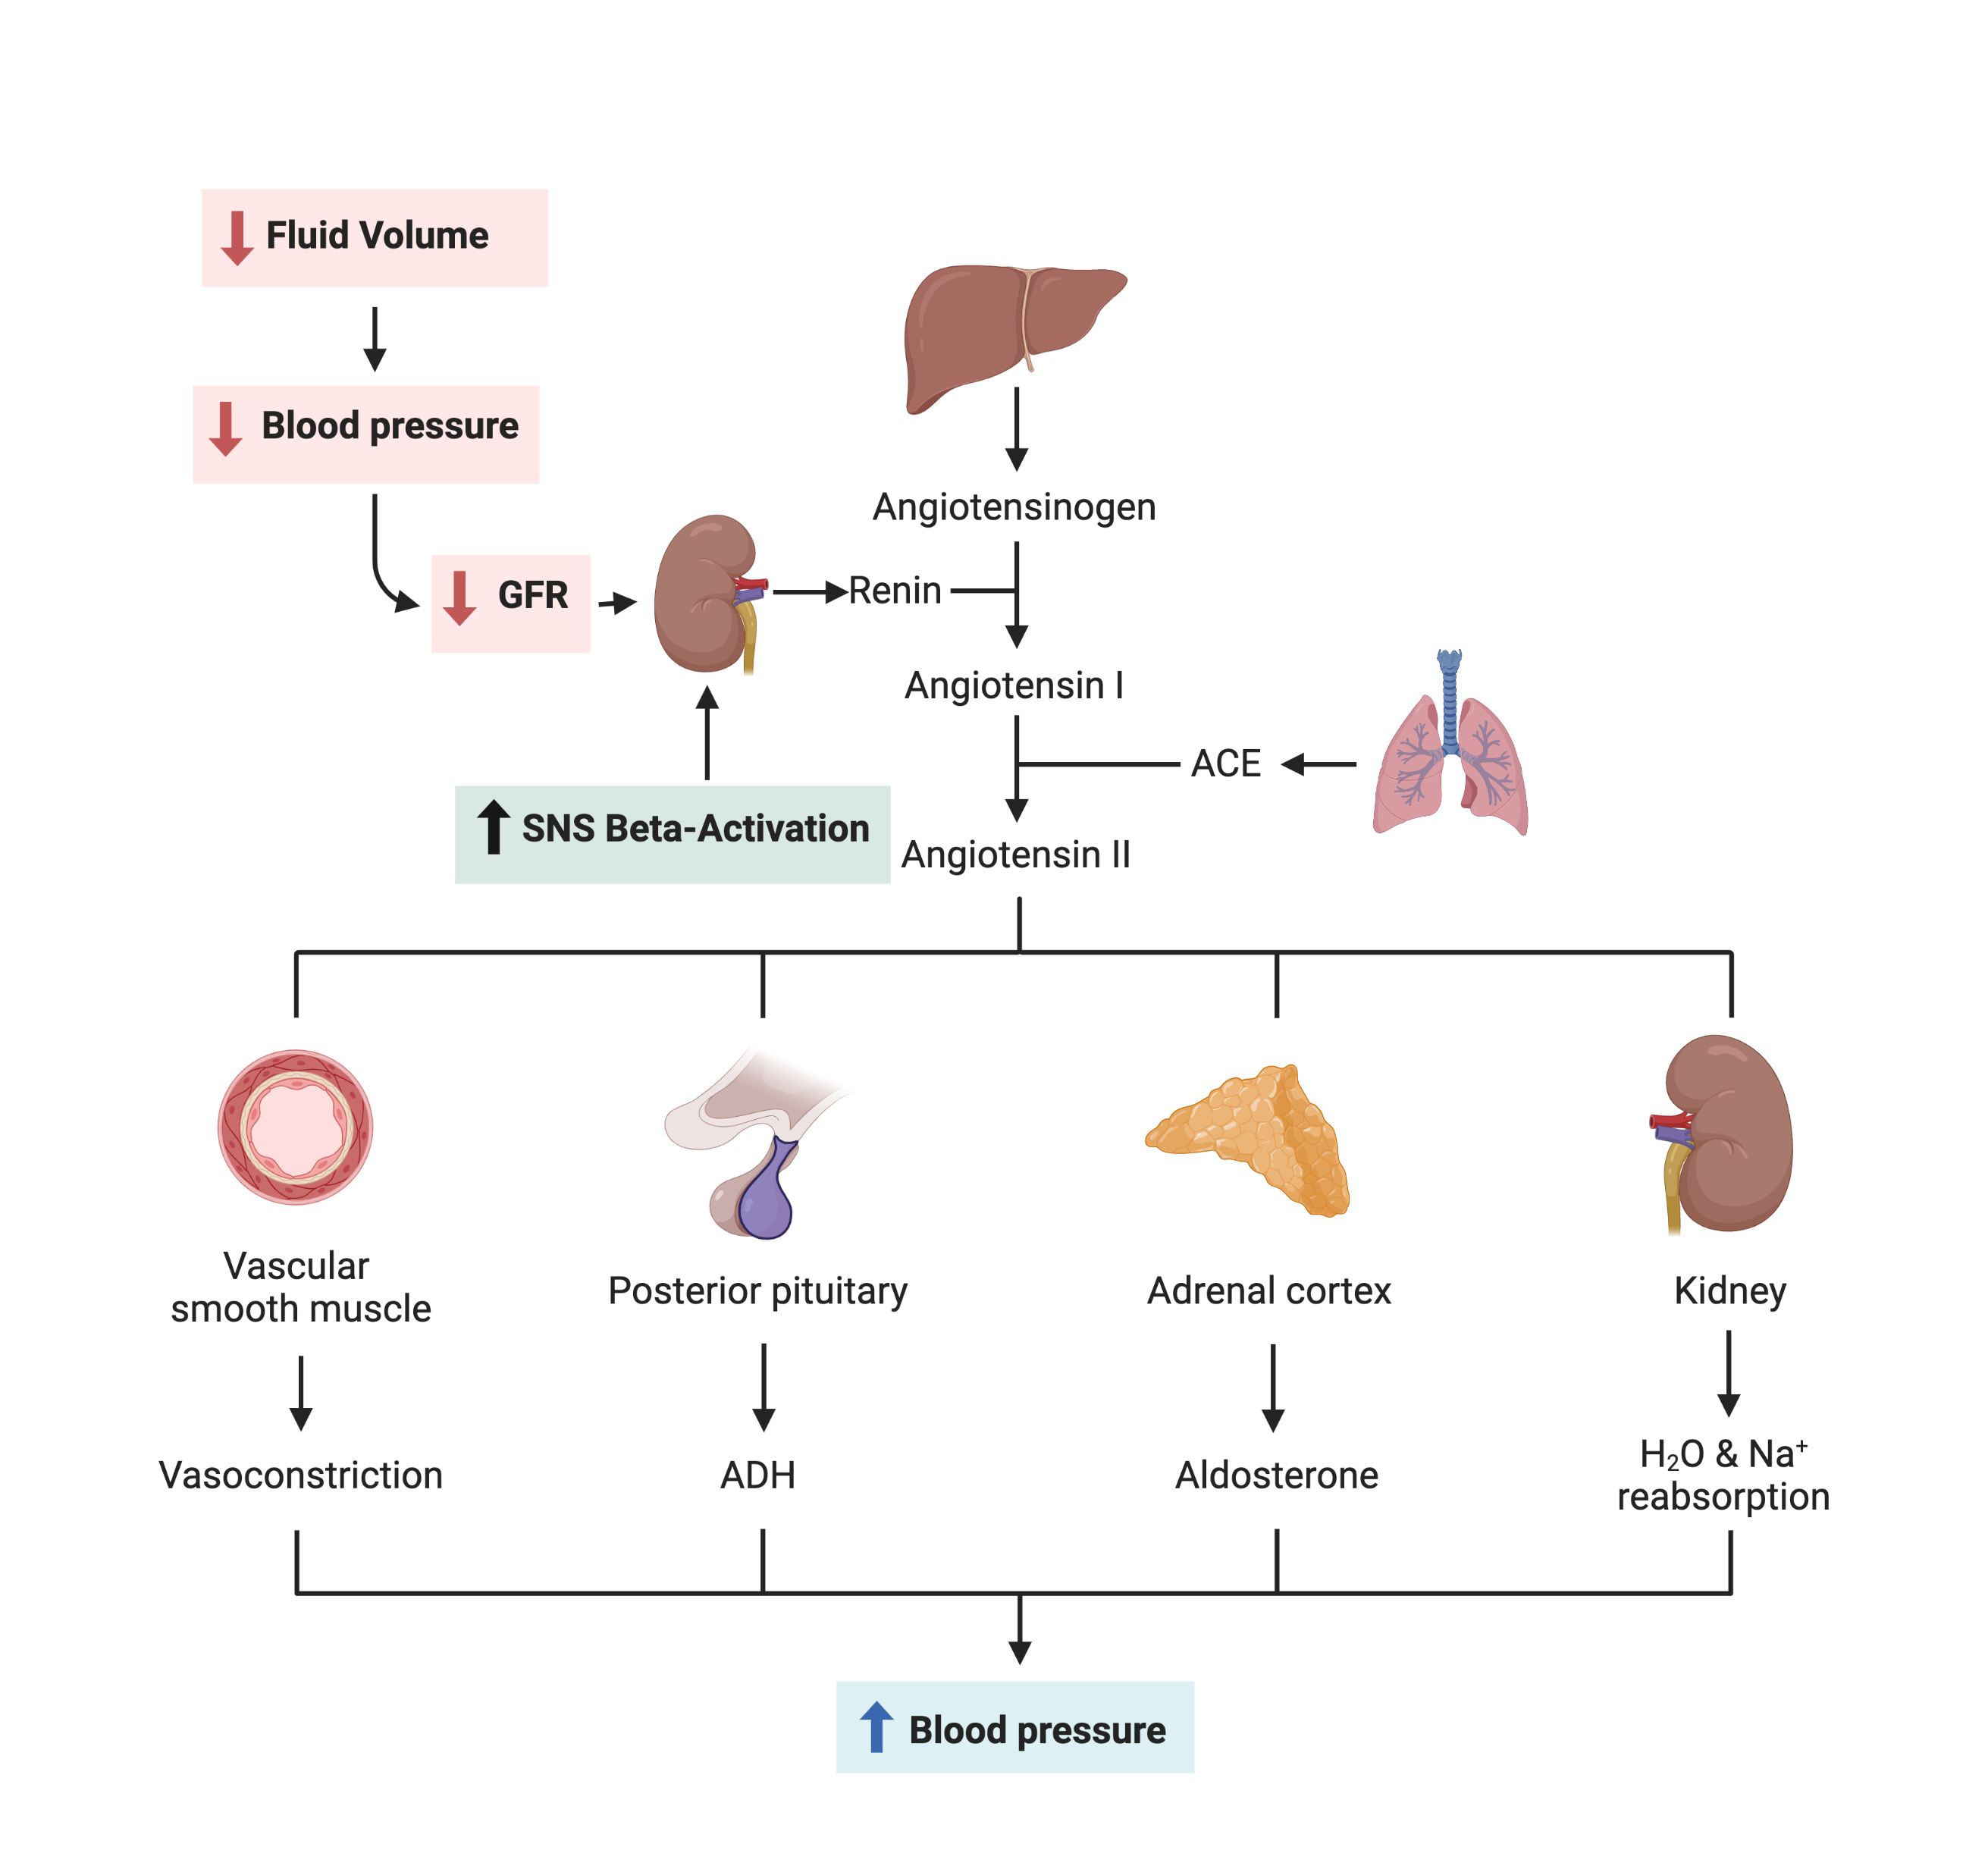
\includegraphics[width=.75\linewidth]{./figure/raas.png}
    \caption{Renin Angiotensin - Aldosterone System (RAAS) \footnotesize{(Created with BioRender.com)}}
    \label{fig:raas}
\end{figure}

\begin{warning}{RAAS Gone Wrong - Heart Failure \& ACE-Inhibition}
    The events of RAAS depicted in Figure \ref{fig:raas} can go wrong. With chronic heart failure (HF) there can be reduced $BP$, or even with preserved $BP$ but lower cardiac output, reduced RBF and GFR, that promotes the secretion of renin by the kidneys. In the context of HF, RAAS increases return of blood to the heart (preload) due to an increased vascular volume. The increased preload adds additional burden to an already failing heart. RAAS also increases the load that the heart must pump against (afterload) due to an increased blood pressure and systemic vasoconstriction. The increased afterload also adds additional burden to an already failing heart. The result tends to be a further reduction in cardiac output and GFR which promotes more renin secretion. This positive feedback loop is far from positive for the health of the individual with HF. In such situations the best course of action for restoring stability is a class of medication referred to a ACE-Inhibitors (ACE-I, i.e. captopril, lisinopril, enalapril) that block the enzyme at converts angiotension I to angiotensin II. ACE-I are also a preferred treatment for HTN (high blood pressure). Rather than forcing diuresis (as a diuretic does, which can create hypokalemia), they prevent anti-diuresis. Anti-anti diuresis is a gentle and physiologically stable approach to diuresis that prevents one of the several deleterious responses to reduced GFR due to HF. The therapuetic benefit of ACE-I goes beyond preventing anti-diuresis and includes reducing the release of aldosterone, and preventing angiotensin II from directly vasoconstricting blood vessels (increasing total peripheral resistance ($TPR$) and diastolic blood pressure (DBP)), and directly resulting in water and $Na^+$ reabsorption.
\end{warning}


\subsubsection{Overall Integration of Renal Mechanisms and Arterial Pressure}

Figure \ref{fig:integrated_renal_bp} is a directed graph that depicts the closed loop integration of renal and circulatory systems through the renal regulation of blood volume, and the arterial pressure influence over renal excretion. 

\begin{figure}[!h]
    \centering
    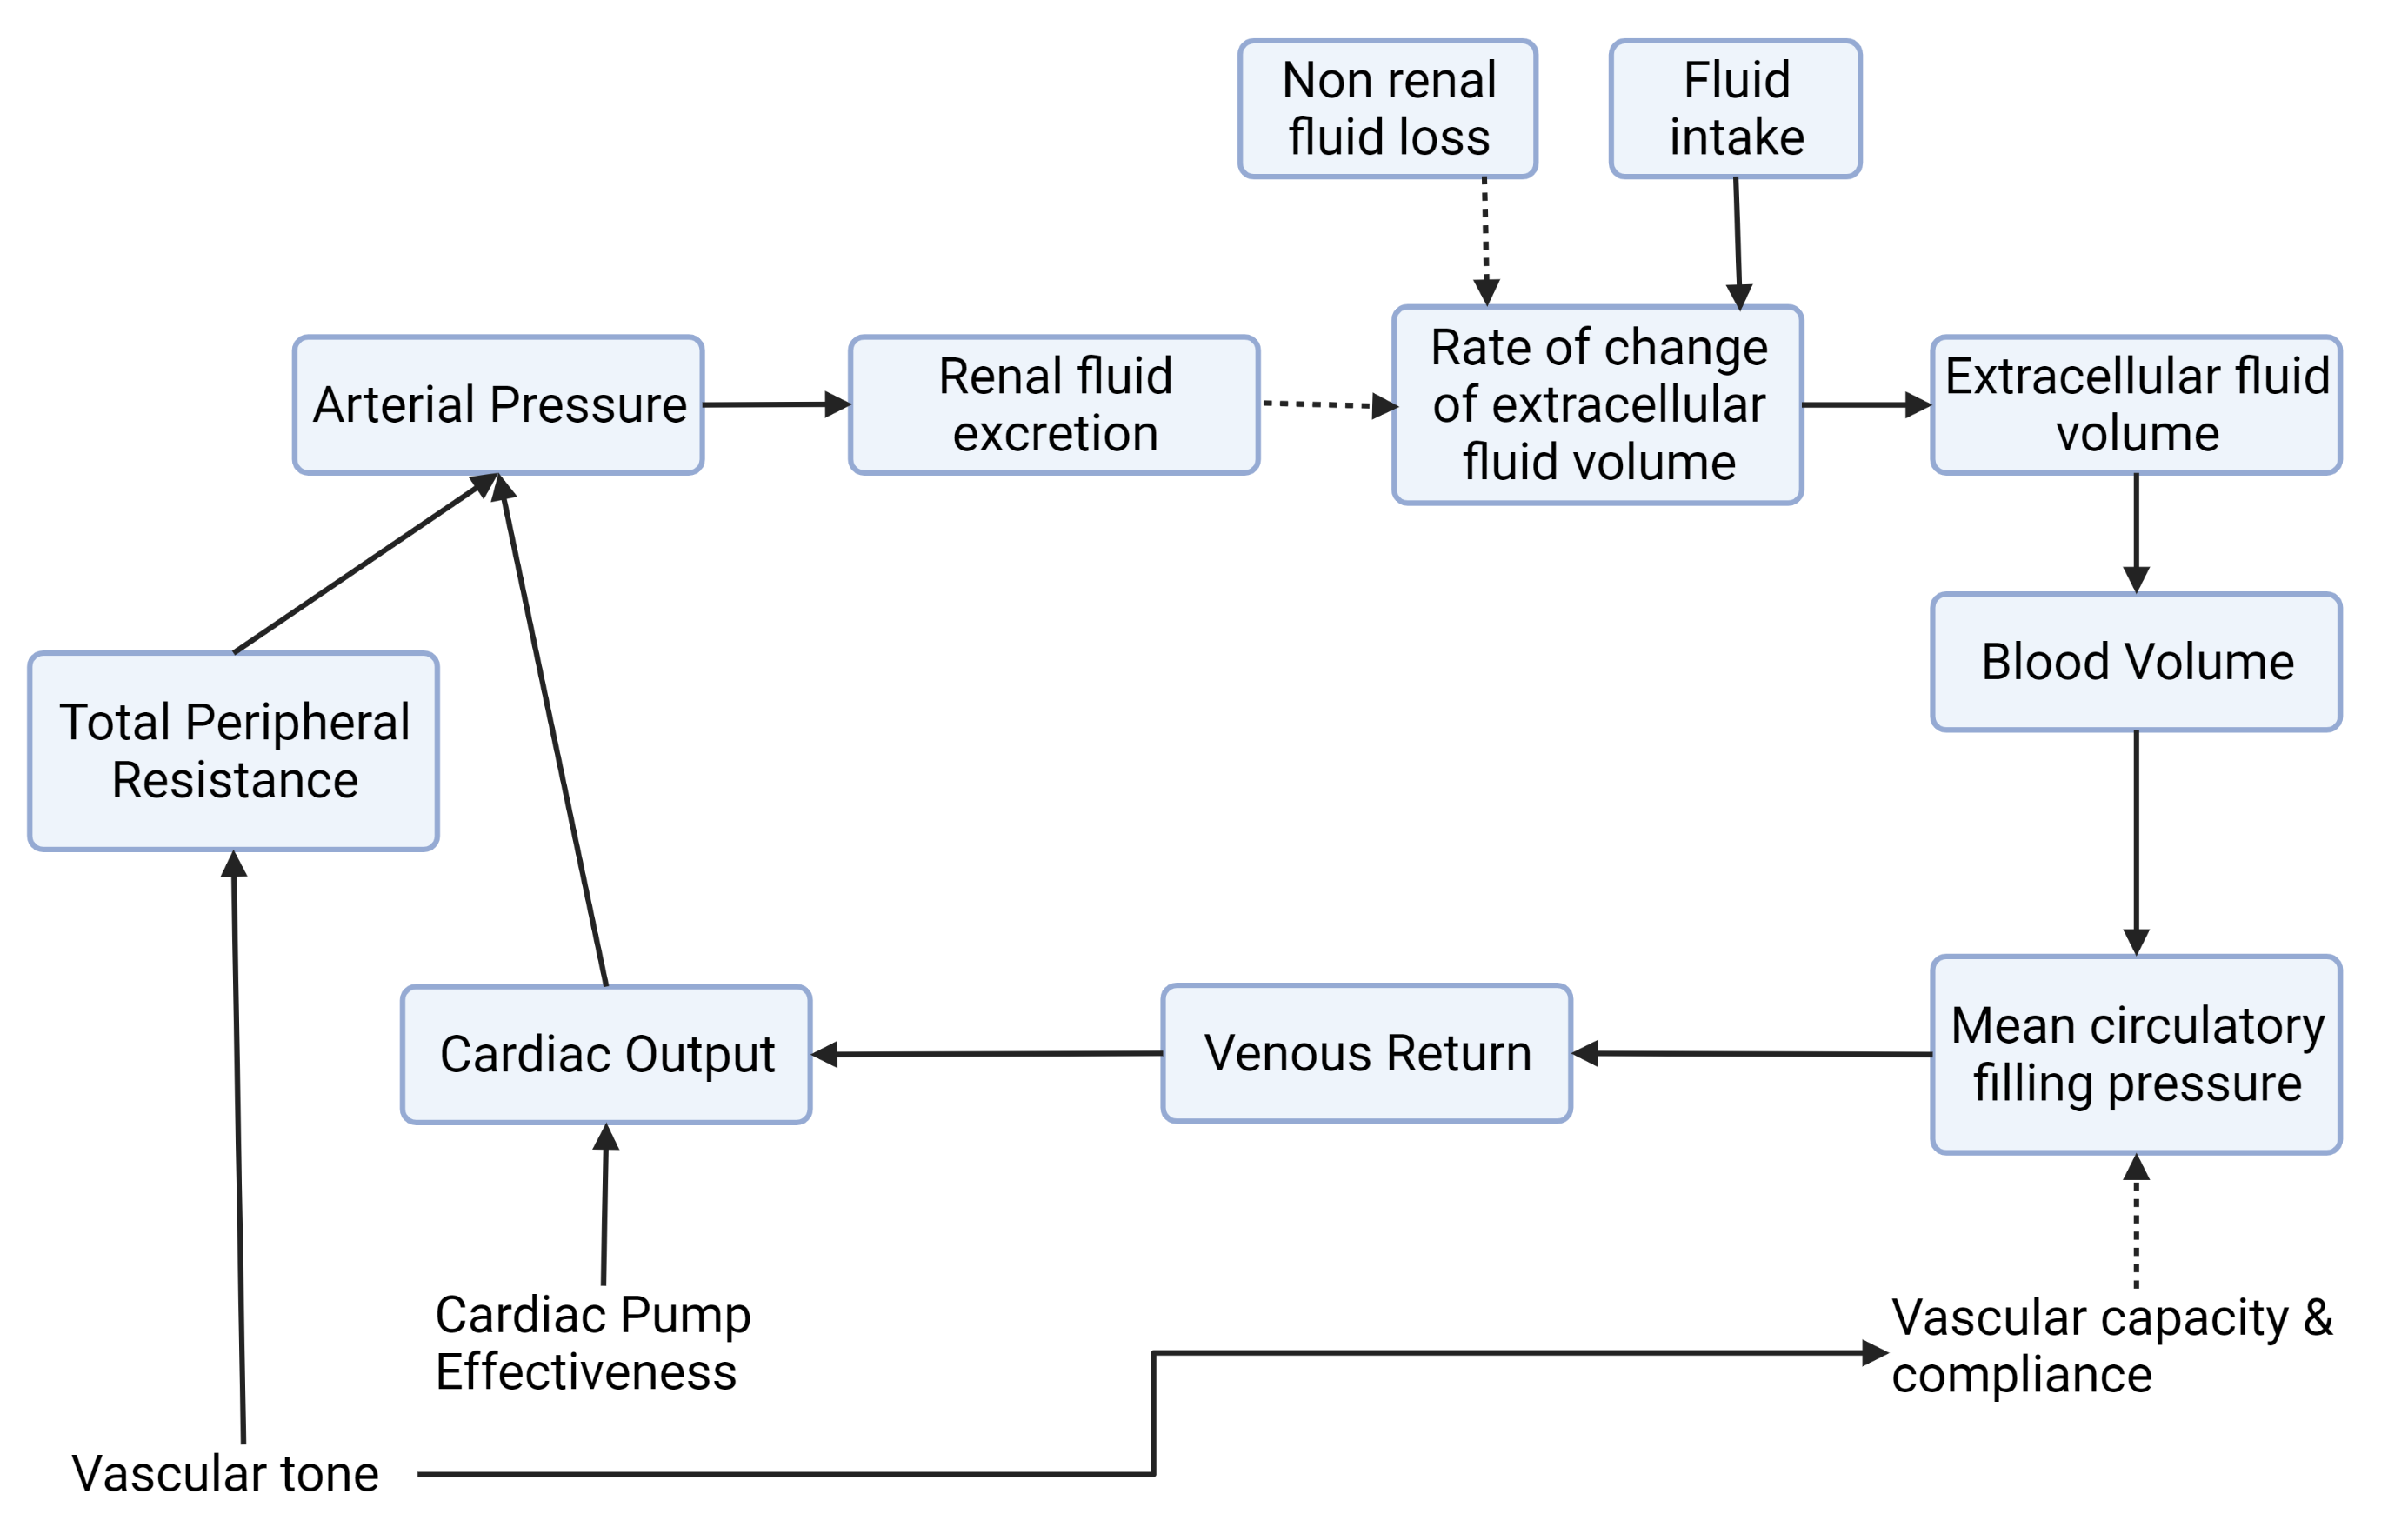
\includegraphics[width=1\linewidth]{./figure/integrated_renal_bp.png}
    \caption{Integration of Renal Mechanisms with Arterial Pressure  \footnotesize{(Modified from \cite{hall_guyton_2020} with BioRender.com)}}
    \label{fig:integrated_renal_bp}
\end{figure}

The variables in Figure \ref{fig:integrated_renal_bp} are familiar other than he mean circulatory filing pressure ($P_{mcf}$). $P_{mcf}$ is a variable created by Guyton in a model of renal blood pressure regulation \cite{rothe_mean_1993}. $P_{mcf}$ is defined as the mean vascular pressure that exists with a stop in cardiac output and distribution of blood until all pressures are the same throughout the system. It is based on the fullness of the circulatory system. A change in $P_{mcf}$ is a useful index of a change in overall venous smooth muscle tone if the blood volume is not changed. $P_{mcf}$ estimates the pressure in the small veins and venules, which contain most of the blood and account for most of the compliance. In total, $P_{mcf}$ provides an estimate of the pressure that determines the rate of flow returning to the heart, independent of cardiac output.

\newpage
\section{Cardiovascular Vital Signs}

\subsubsection{Palpation of Pulses} 
Palpation of pulses is an important component of a physical examination and can be used to evaluate and identify the following:

\begin{itemize}
\item Circulation quality
\item Pulse rate and rhythm
\end{itemize}

\paragraph{Circulation Quality}

Pulse are pressure waves through the circulation that are related to both blood pressure and local circulation. Weak pulses can indicate either low blood pressure (overall) or poor circulation that particular region of the body. For example, a weak pulse in the right radial artery but not the left radial artery most likely indicates a local circulation problem in the left UE but not the right. Whereas a weak pulse in all extremities is most likely a low blood pressure overall. A strong, or bounding, pulse can indicate a high blood pressure overall, or a high blood pressure in a particular area. Bounding pulses can also indicate vascular abnormalities such as aneurysms (for example a bounding abdominal pulse is a sign of a descending aortic aneurysm).

\paragraph{Heart Rate \& Rhythm}

Pulses are correlated with heart rate (cardiac cycle) and rhythm. When palpating a pulse to obtain $HR$, counting the pulse rate for 15 seconds and multiplying by 4 is sufficient with normal rates and rhythms. If rates are faster than 100 bpm or slower than 60 bpm, palpate the pulse for 60 seconds. If the rhythm is irregularly irregular (e.g., during AFib) or regularly irregular (e.g., PACs or PVCs), perform auscultation of heart sounds to identify the apical $HR$ for a full minute. In these cases, palpation of pulse cannot substitute for ECG analysis to monitor the patient’s rhythm, but it may alert the therapist to the onset of these abnormalities.

Use caution in palpating pulses because manual pressure on the carotid sinus may cause baroreflex drops in heart rate ($HR$), blood pressure ($BP$), or both. In all pulse palpation situations the examiner should start with light pressure and gradually increase pressure until a pulse is felt, and to not exert more pressure than required to feel the pulse.

Some people can feel a pulse in their thumb, therefore it is generally advised to not use the thumb to palpate a pulse.

$HR$ is the primary means of determining the exercise intensity level for patients who are not taking beta-blockers or who have rate-responsive pacemakers. $HR$ combined with blood pressure (RPP) is the most appropriate approach to determine exercise intensity in any patient with a known ischemic threshold (even if they are on beta-blockers).

\begin{itemize}
\item A linear relationship exists between $HR$ and work.
\item In general, a 20- to 30-beat increase from the resting value during activity is a safe intensity level in which a patient can exercise.
\item If a patient has undergone an exercise stress test during the hospital stay, a percentage (e.g., 60\%–80\%) of the maximum $HR$ achieved during the test can be calculated to determine the exercise intensity.
\item An example of a disproportionate $HR$ response to low-level activity (bed or seated exercises or ambulation in room) is an $HR$ of more than 120bpm or less than 50bpm.
\item Heart rate recovery ($HRR$), provides an indication of reduced parasympathetic activity and an indicator of all-cause mortality, can be used to document improvement of tolerance to functional demands. $HRR$ is the absolute difference between peak HR achieved with exercise minus the $HR$ at 60 seconds after the completion of exercise ($HRR$ 60 sec).  An abnormal $HRR$ at 1 minute, after a treadmill test, is reported to be a decrease of 12 bpm or less with a cool-down period and less than 18 bpm without a cool-down period \cite{collins_cardiac_2019}.
\item When prescribing activity intensity for a patient taking beta-blockers, consider that $HR$ should not exceed 20 beats above the resting $HR$. If RPP for the patient's ischemic threshold is known, then the RPP should not be allowed to increase to the ischemic threshold.
\item If prescribing an activity intensity, with use of $HR$, for patients with an automatic implantable cardiac defibrillator (AICD), remember that the exercise target $HR$ should be 20 to 30 beats below the threshold rate on the defibrillator.
\item $HR$ should not be used to prescribe exercise status post heart transplantation secondary to denervation of the heart during transplantation.
\item Baseline $HR$ and recent changes in medications always should be considered before beginning an exercise session.
\end{itemize}

\subsubsection{Blood Pressure}

Blood pressure is critical to circulation and a primary variable utilized to help regulate cardiac output. Low blood pressure (and low PP) is problematic because it compromises circulation and may indicate hemodynamic compromise due to cardiac (reduced cardiac output), vascular (reduced peripheral resistance) or blood volume problems. High blood pressure can create immediate health care emergencies by placing blood vessels under too much pressure; or cardiac emergencies by causing ischemia (high RPP and myocardial $O_2$ demand), or heart failure (increased afterload). Long term increased high blood pressure (hypertension) leads to long term changes in the heart (left ventricular hypertrophy, fibrosis of the atria and ventricles that makes the heart more susceptible to arrhythmias, or valve dysfunction). Hypertension is a silent killer since many individuals have no idea they have it - which is one of the reasons for the APTA Academy of Cardiovascular and Pulmonary Physical Therapy's "Vitals are Vital" campaign to encourage all physical therapists in all settings to make sure they routinely examine vitals signs in all clients.

Measurement of $BP$ with a sphygmomanometer (cuff) and auscultation is an indirect, noninvasive measurement of the force exerted against the arterial walls during ventricular systole (SBP) and during ventricular diastole (DBP). $BP$ is affected by total peripheral resistance (blood volume, radius and compliance of arterial walls) and $\dot{Q}$. Table \ref{table:BP_Ranges} includes normal $BP$ ranges. 

\begin{table}[h!]
\centering
\begin{tabular}{||c c c ||} 
 \hline
 Ranges & Systolic (mmHg) & Diastolic (mmHg) \\ [0.5ex] 
 \hline\hline
Age 8 years & 85-114  & 52-85  \\ 
Age 12 years & 95-135  & 58-88   \\
Adult & $<$ 120   & $<$ 80   \\
Elevated (Adult) & 120-129   & $<$ 80  \\
Stage 1 Hypertension & 130-139  & 80-89   \\
State 2 Hypertension & $\geq$ 140 &  $\geq$ 90 \\ [1ex] 
 \hline
\end{tabular}
\caption{Blood Pressure Ranges, Modified from \cite{collins_cardiac_2019}}
\label{table:BP_Ranges}
\end{table}

Occasionally, $BP$ measurements can be performed only on certain limbs secondary to the presence of such conditions as a percutaneously inserted central catheter, arteriovenous fistula for hemodialysis, blood clots, or lymphedema (e.g., status post mastectomy). 

$BP$ of the upper extremity should be measured in the following manner \cite{collins_cardiac_2019}:

\begin{enumerate}
\item Check for posted signs, if any, at the bedside that indicate which arm should be used in taking $BP$. $BP$ variations of 5 to 10 mmHg between the right and left upper extremity are considered normal. Patients with arterial compression or obstruction may have differences of more than 10 to 15 mmHg.
\item Use a properly fitting cuff. The inflatable bladder should have a width of approximately 40\% and length of approximately 80\% of the upper arm circumference.
\item Position the cuff 2.5 cm above the antecubital crease.
\item Rest the relaxed arm at the level of the heart.
\item To determine how high to inflate the cuff, palpate the radial pulse, inflate until no longer palpable, and note the cuff inflation pressure. Deflate the cuff. This is an estimate of the systolic pressure. But this method cannot be utilized to obtain a diastolic pressure.
\item Place the bell of the stethoscope gently over the brachial artery.
\item Reinflate the cuff to 30 to 40 mmHg greater than the value in step 5. Then slowly deflate the cuff. Cuff deflation should occur at approximately 2 to 3 mmHg per second.15
\item Listen for the onset of tapping sounds, which represents circulation returning to the brachial artery. This is the SBP.
\item As the pressure approaches diastolic pressure, the sounds will become muffled and in 5 to 10mmHg will be completely absent. These sounds are referred to as Korotkoff sounds (See Table \ref{Korotkoff}).
\end{enumerate}

\begin{table}[h!]
\centering
\begin{tabular}{||c c c ||} 
 \hline
 Phase & Korotkoff Sound & Indicates \\ [0.5ex] 
 \hline\hline
1  & First sound, faint tapping  & Systolic pressure (circulation through compressed artery)  \\ 
2  & Blowing or swishing sound  & Blood is increasing   \\
3 & Distinct tapping   & Circulation is increasing   \\
4 & Muffled  & Diastolic pressure in certain situations$^a$\\
5 & Disappearance  & Diastolic pressure in adults   \\ [1ex] 
 \hline
\end{tabular}
\caption{Blood Pressure Ranges ($^a$ \footnotesize{Phase 4 represents DBP in children, and adults that are exercising, pregnant or with hyperthyroid conditions})(Modified from \cite{bickley_bates_2012})}a
\label{Korotkoff}
\end{table}

\paragraph{Systolic Blood Pressure / Palp}

In situations when it is difficult to auscultate or to obtain a distinct diastolic blood pressure reading (DBP), the palpation method may be utilized and blood pressure is noted as systolic blood pressure (SBP)/Palp. This is the same procedure utilized in Step 5 to determine how high to pump the cuff for a full measurement of blood pressure without having to over inflate the cuff.


\subsection{Physical Therapy Considerations}
\begin{itemize}
\item Recording pre exertion, para exertion, and post exertion $BP$ is important for identification of $BP$ responses to activity. During recovery from exercise, blood vessels dilate to allow for greater circulation to muscles. In cardiac-compromised or very deconditioned individuals, total $\dot{Q}$ may be unable to support this increased flow to the muscles and may lead to decreased output to vital areas, such as the brain.
\item If you are unable to obtain $BP$ on the arm, the thigh is an appropriate alternative, with auscultation at the popliteal artery.
\item Falsely high readings occur if the cuff is too small or applied loosely or if the brachial artery is lower than the heart level.
\item Evaluation of $BP$ and $HR$ in different postures can be used to monitor orthostatic hypotension with repeat measurements on the same arm 1 to 5 minutes after position changes.
\item The same extremity should be used when serial $BP$ recordings will be compared for an evaluation of hemodynamic response.
\item A $BP$ record is kept on the patient’s vital sign flow sheet. This is a good place to check for $BP$ trends throughout the day and, depending on your hospital’s policy, to document $BP$ changes during the therapy session.
\item An auscultatory gap is the disappearance of sounds between phase 1 and phase 2 and is common in patients with high $BP$, venous distention, and severe aortic stenosis. Its presence can create falsely low SBPs if the cuff is not inflated enough (prevented by palpating for the disappearance of the pulse before measurement), or falsely high DBPs if the therapist stops measurement during the gap (prevented by listening for the phase 3 to phase 5 transitions).
\item In general there is a lower SBP, higher DBP, and lower workload at any given submaximal $HR$ during arm exercise compared with leg exercise \cite{dias_differences_2022}
\item A clearly disproportionate response to exercise includes SBP decrease of 10 mmHg below the resting value, a hypertensive systolic response of greater than 200 mmHg, or a hypertensive diastolic response of greater than 110 mmHg. A normotensive systolic blood response should increase 5 to 12 mmHg per increase in metabolic equivalents (METs). One MET is approximately 3.5 ml/kg/min of oxygen consumption.
\item If the patient is on a pacemaker that does not have heart rate modulation, $BP$ response can be used to gauge intensity. 
\end{itemize}


\section{Summary}

This chapter has provided introduced circulation from the perspective of cardiac output. The focus has been on the systemic circulation, what leaves the left ventricle and returns to the right atria without much consideration of what the heart is doing in its role as a pump. We simply took it for granted that the heart pumps a volume of blood out with each beat ($SV$) and it does so a certain number of times per minute ($HR$). 
Circulation is measured by us as cardiac output but is sensed physiologically by the indirect means of $BP$. Homeostatic mechanisms are in place that allow the monitoring of $BP$ to adjust of $HR$ (chronotropy), $SV$ through cardiac contractility (inotropy) and venous return (vascular tone through neuroendocrine mechanisms), blood volume (renal and renal endocrine mechanisms) and $TPR$. Monitoring $BP$ and $HR$ provide physical therapists with non-invasive insights. When combined with an understanding of circulatory physiology these insights provide useful information when working with clients both with and without conditions that directly affect the circulation.

\subsection*{Next Step - The Cardiac Pump}

In Chapter \ref{chp:cardiac_pump} on the Cardiac Pump we fill in the gap of circulation between the blood entering the right atrium and the blood leaving the left ventricle. This includes the factors the influence heart rate, stroke volume; properties of the cardiac muscle; cardiac circulation and the electrocardiograph to assess cardiac function.

\printbibliography[heading=subbibintoc]

\section*{Sample Questions}

\begin{enumerate}
    \item Based on Poiseuille’s Law which factor has both a strong and a highly variable (physiologically adjustable) determinant of peripheral resistance?
    \item How is central venous (right atrial) pressure kept at approximately 0?
    \item What factors allow the distribution of cardiac output to respond to metabolic demands?
    \item What are the implications associated with changes in vascular tone based on altered sympathetic nerve activity change vessel radius and compliance in the same direction (both increase or both decrease)?
    \item What is the sequence of events based on the baroreceptor response to standing up from supine?
\end{enumerate} 
% !TEX root = ../notes_template.tex

\chapter{Cardiac Pump}\label{chp:cardiac_pump}
Updated on \today
\minitoc
This chapter covers the cardiac pump in its role to support circulation. Circulation is completely dependent on the pumping action of the cardiac muscle to create the pressure gradient for both systemic, and a bit less so, the pulmonary circulation. 

The relationship between circulation and cardiac muscle is similar to the relationship between movement and skeletal muscle. Concepts from skeletal muscle such as tension, excitation, regulation and energetics are applicable to cardiac muscle and are included. It is useful to compare and contrast cardiac muscle with skeletal muscle across these concepts while focusing on how the differences enable the cardiac muscle to meet the unique needs of circulation. The primary goal of this chapter is an understanding of cardiac pump in its supportive role for circulation. 

\vspace{5mm}
\begin{svgraybox}
\textbf{Objectives include:}
\begin{enumerate}
    \item Compare and contrast cardiac and skeletal muscle based on tension, excitation, regulation and energetics.
    \item Explain how the unique characteristics of cardiac muscle tension, excitation (automaticity, rhymicity, conductivity, contractility), regulation and energetics support circulation.
    \item Explain factors that influence cardiac output (including preload, afterload, intropy, chronotropy).
    \item Explain the relationship between RPP and myocardial oxygen demand.
    \item Explain cardiac circulation.
    \item Explain the cardiac cycle (to the point of drawing and explaining all aspects of Wiggers Diagram).
    \item Perform an ECG rhythm analysis including the identification of arrhythmias and myocardial circulation abnormalities.
\end{enumerate}
\end{svgraybox}

\section{Cardiac Muscle}

The role of the heart as a pump is based on it's ability to regularly provide the pressure necessary for circulation of blood through arterial vessels (both systemic arteries (which includes the cardiac circulation) and pulmonary arteries). The function of the heart as a pump depends on several characteristics of cardiac muscle:

\begin{itemize}
    
    \item Automaticity: The ability to initiate its own excitation
    \item Rhythmicity: The ability to repeat the its own excitation cycle in synchrony with regularity
    \item Excitability: The ability to respond to excitation with activation
    \item Conductivity: The ability to transmit excitations from cell to cell within the heart
    \item Contractility: The ability to generate a full contractile (shortening) cycle with each excitation
 
\end{itemize}

The next four sections parallel the chapters on skeletal muscle function of Part II: Tension, Excitation, Regulation and Energetics. They, in turn, compare and contrast cardiac and skeletal muscle in these key areas and also how the cardiac muscle and pump are thus uniquely capable of supporting circulation. As a reminder Chapter \ref{chp:circulation} on Circulation focused on circulation leaving the left ventricle and returning to the right atrium. This chapter is focused on the circulation through the heart itself as it is pumped and travels from the right atrium to the left ventricle. There are, however, two caveats. First, this chapter includes details about the cardiac circulation within the section on energetics (since cardiac muscle energetics is very dependent on the regular delivery of oxygen via blood flow). Second, this chapter does not include details on the pulmonary circulation (leaving the right ventricle and returning to the left atrium). The pulmonary circulation is covered in the next chapter on Respiration.

\subsection{Tension}

It is reasonable to use the term contraction when describing activation and active tension for the cardiac muscle because contraction (shortening) is what occurs (there is no eccentric or isometric activation of cardiac muscle). A major difference between cardiac and skeletal muscle is that cardiac muscle does not have a tendon attachment. Cardiac muscle attaches to itself to create a chamber that has a volume. When cardiac muscle contracts, it makes the chamber smaller (less volume). In skeletal muscle the length of fibers translates into the length of the entire muscle and this relationship has a functional interpretation. In cardiac muscle the length of fibers directly translates into the volume of chambers. It is the volume of these chambers that has a functional interpretation. 

The heart has four chambers that function as four pumps (right and left atria; right and left ventricles). From a muscular perspective there are two chambers, each separated into a right and a left side with a relatively thin muscular barrier between them. This is quite noticeable in conditions that result in abnormal timing of the right and left ventricle excitation. If the ventricles are not excited at the same time, off even by 50 milliseconds, the overall pump effectiveness of both ventricles is impaired (mechanical cardiac asynchrony).

\paragraph{Active Tension}

Active tension is generated in cardiac muscle with the same sliding filament model of skeletal muscle described in Chapter \ref{chp:tension} on Tension. Active tension generates tension that shortens cardiac muscle fibers and makes the cardiac chambers smaller (and less compliant). 

\paragraph{Passive Tension}

Passive tension is generated by titin and other connective tissue structures that resist lengthening of sarcomeres, which in turn resists enlarging the chamber. Passive tension also attempts to shorten cardiac muscle fibers when they are stretched (lengthened fibers when the chamber has a larger volume). Additional passive tension is developed by layers of connective tissue surrounding the heart including the epicardium (visceral layer of the serous pericardium), the parietal layer of the serous pericardium, and the fibrous pericardium (See Figure \ref{fig:Cardiac_Muscle}). The pericardial cavity is filled with pericardial fluid which reduces friction during the cardiac cycle of contraction - relaxation. All of these structures, including the amount of fluid in the pericardial fluid, impact the compliance of the heart chambers.

\begin{figure}[!h]
    \centering
    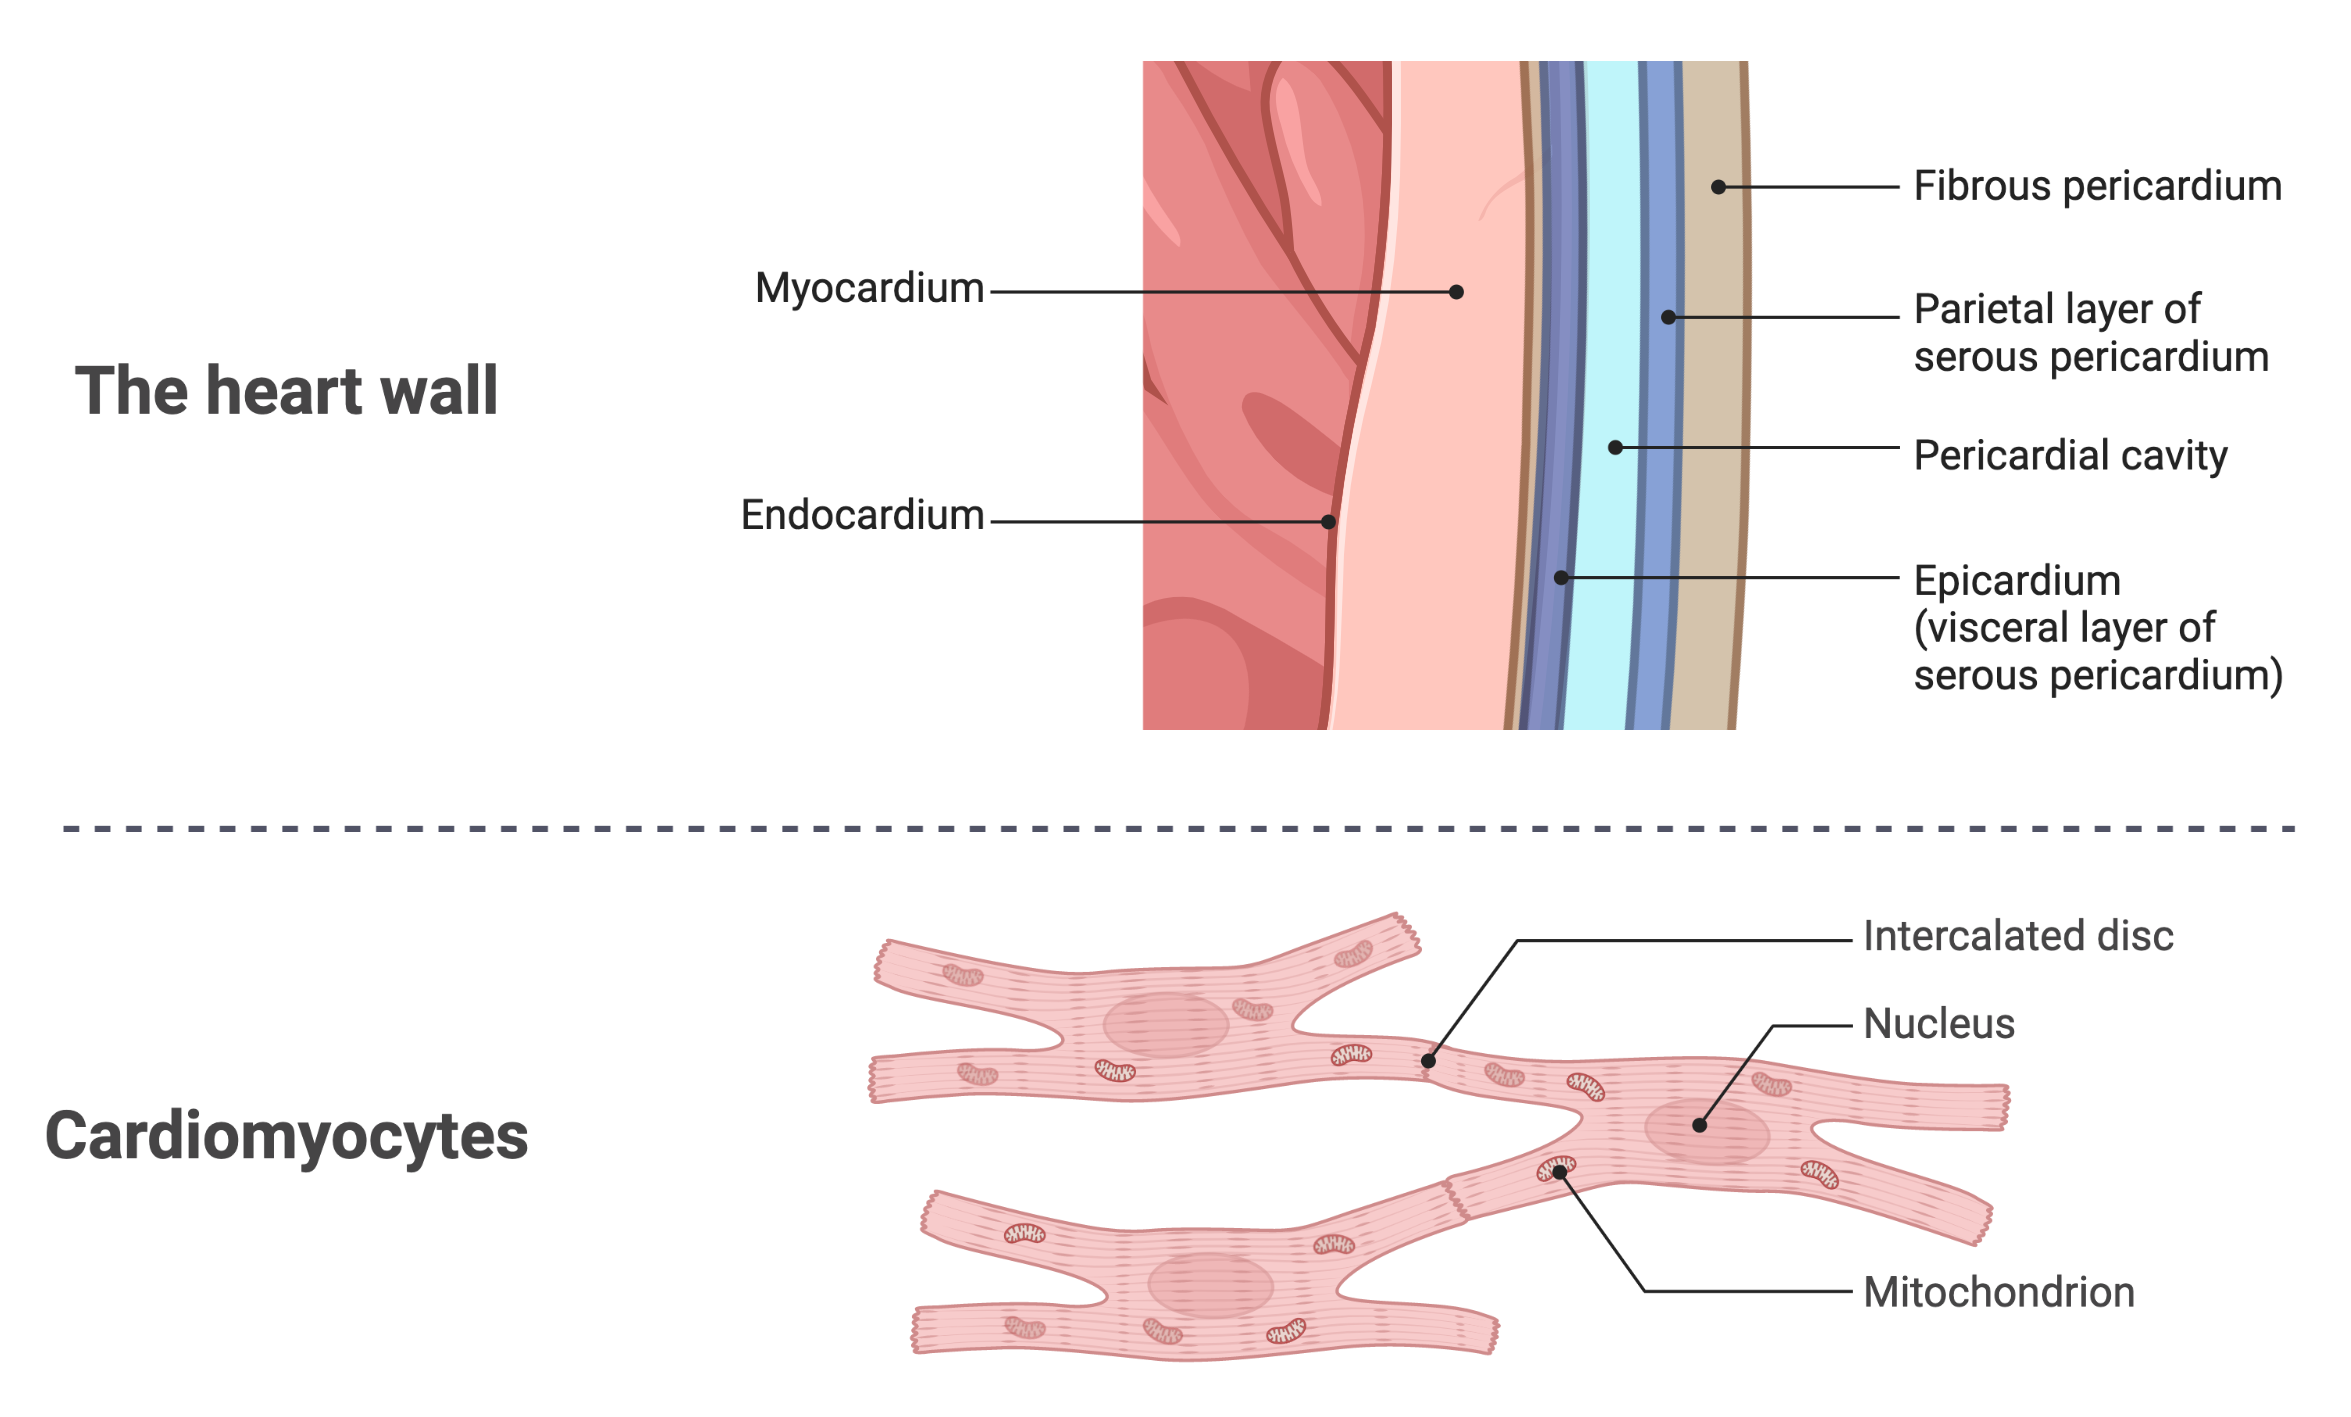
\includegraphics[width=.75\linewidth]{./figure/Cardiac_Muscle.png}
    \caption{Cardiac Muscle \footnotesize{(Created with BioRender.com)}}
    \label{fig:Cardiac_Muscle}
\end{figure}

\paragraph{Volume-Tension Curve}

Cardiac muscle fibers \textit{in vitro} have a length-tension curve that is similar to skeletal muscle fibers. The primary difference is that the passive component is shifted to the left and is a steeper exponential curve. The active component displays a similar curve based on the overlap of actin and myosin. The passive component displays that cardiac muscle has a stiffer form of titin that contributes to tension with a smaller increase in length. 

Cardiac muscle \textit{in situ} has a \textbf{volume-tension curve} that is synonymous with the length-tension curve of whole skeletal muscle. The cardiac volume-tension curve is similar looking to its length-tension curve, the primary difference again being the passive component is shifted further to the left and is steeper. The volume-tension curve is influenced by the length-tension of the cardiac muscles and the passive structures surrounding the heart that resist changes in the chamber size directly. Passive tension starts to develop as the cardiac chamber fills. The functional implication is that under normal resting conditions passive tension contributes to cardiac contraction. And with larger volumes of blood in the chambers the contribution of passive tension rises exponentially.

The passive component of the volume-tension curve is related to cardiac compliance. As described in Chapter \ref{chp:microcirculation} there is a relationship between volume, compliance and pressure. The cardiac muscles vary the volume of chambers while having a particular compliance (that varies with the passive and active tension) for the purpose of generating pressure. This is a fundamental difference between cardiac and skeletal muscle tension. Skeletal muscle tension changes length based directly on tension for the purposes of generating torque. Cardiac muscle tension changes length for the purpose of changing volume and compliance, for the purpose of changing pressure. It is the pressure generated in the cardiac chambers that result in circulation.

Understanding cardiac function requires a familiarity with the equations relating compliance, volume and pressure introduced in Chapter \ref{chp:microcirculation}, repeated here specific for the heart:

\begin{equation}
    \Delta P_{chamber} = \frac{\Delta V_{chamber}}{C_{chamber}}
    \label{eq:Cardiac_Pressure}
\end{equation}

In Equation \ref{eq:Cardiac_Pressure} the dependency of pressure on volume and compliance is clear. Since circulation is a cyclic variation in pressure gradients through the cardiac pump (and vascular vessels), the entirety of cyclic circulation through the heart can be considered from the perspective of cyclic changes to volume and compliance that develop pressure gradients to create flow through and out of the heart. Consideration of volume and compliance for the function of the heart a a pump correctly orients the discussion for both active and passive tension since they both contribute to cardiac pump function.

\subsubsection{Preload}

Preload is the term given for the pressure in a chamber when the cardiac muscle is filled (circulation into the chamber is approaching 0) but is not yet activated. Preload is the passive tension in the chamber right before it develops active tension. Preload for cardiac muscle is analogous to stretch on skeletal muscle. The pressure of preload is related to the volume and the compliance. The compliance is at its highest when the myocardium is empty and not activated. As the chamber fills with blood, passive tension starts to develop which gradually reduces compliance while increasing the volume of blood, which when combined increases pressure. Under normal circumstances this increase in pressure (higher blood volume and lower compliance) is not great enough to fully impede circulation into the chamber. The passive tension developed during preload is subsequently utilized to assist active tension. Which develops the tension necessary to change the volume and compliance of the chamber for the purpose of increasing pressure to facilitate circulation out of the chamber. The increased pressure, alone, simply directs circulation out of the chamber from an area of high to low pressure. The direction of actual circulation through the heart is dependent on properly functioning valves that limit flow "backwards" and allow circulation "forwards" based on cardiac anatomy (Figure \ref{fig:Cardiac_Anatomy}.

The preload is directly related to end-diastolic pressure (EDP), which is directly related to end-diastolic volume (assuming the compliance is normal and relatively low during diastole). The volume that results in preload is from circulation. Where the circulation is coming from for preload depends on the chamber. The right atrium preload comes from the systemic veins; right ventricle preload comes from the right atrium through the tricuspid valve; left atrium preload comes from the pulmonary veins; left ventricle preload comes from the left atrium through the mitral valve. 

It is most common to discuss preload from the perspective of the left ventricle (LV). Therefore, unless otherwise noted, EDV and EDP mean LVEDV and LVEDP (respectively). EDP is related to the \textbf{Frank-Starling law} which states that the amount of venous return influences the performance of the left ventricle (assumes all the venous return moves through the right heart circulation (RA, RV, pulmonary arteries, pulmonary capillaries, pulmonary veins to the LA and finally the LV). The Frank-Starling mechanism is based on the relationship between EDP and total tension developed from active and passive tension.

\subsubsection{Afterload}
Afterload is the term given for the pressure that a chamber must overcome to cause circulation out of the chamber. Afterload for cardiac muscle is analogous with resistance (or load) for skeletal muscle. It is the resistance that the cardiac chamber must exert its tension in order to reduce the volume of the chamber. The pressure of afterload depends on which chamber must overcome that pressure. For the RA it is the pressure exerted on the tricuspid valve by the RV; for the RV it is the pressure exerted on the pulmonic valve by the pulmonary arteries; for the LA it is the pressure exerted on the mitral valve by the LV; for the LV it is the pressure exerted on the aortic valve by the aorta (first of the systemic arteries). 

It is most common to discuss afterload from the perspective of the LV. Therefore, unless otherwise noted, afterload refers to aortic pressure and is best estimated as mean arterial pressure (MAP) (See Equation \ref{eq:MAP_simplified}). MAP is related to vascular compliance and resistance. As afterload, MAP affects aortic valve opening and is the most obvious load encountered by the ejecting ventricle. 

\begin{warning}{HFpEF}
   Long term high blood pressure (hypertension) results in left ventricular hypertrophy (LVH) that is associated with a reduced size and reduced compliance of the LV chamber. LVH is a common cause of diastolic (preserved ejection fraction (pEF)) heart failure (HFpEF).
\end{warning}

\paragraph{Ejection Fraction}

The amount of blood ejected from the LV during systole is called stroke volume (SV). It should be clear that SV is impacted by both preload and afterload. SV is simply the EDV minus the end systolic volume (ESV) ($EDV-ESV$). 

The percentage of blood in the chamber (EDV) that is ejected during systole is the ejection fraction: 

\begin{equation}
    EF = \frac{SV}{EDV}
    \label{eq:LVEF}
\end{equation}

A useful equation to remember for SV is therefore:

\begin{equation}
    SV = EDV \times EF
    \label{eq:SV}
\end{equation}

Equation \ref{eq:SV} highlights how the two phases of the cardiac cycle (systole and diastole) contribute to stroke volume. Diastole contributes with a volume of blood (EDV). Systole contributes the tension to eject a fraction of that blood (LVEF). As discussed above, LVH can cause something called diastolic or preserved EF heart failure (pEF). That is because LVH reduces SV by reducing the size of the LV chamber. It reduces EDV, but does not reduce LVEF. There are also causes of HF that do reduce LVEF and they are called systolic or reduced EF heart failure (rEF). There are also situations - most often due to comorbidities (having more than one condition) - that cause HF with both diastolic (reduced EDV) and systolic (reduced LVEF) components. 

\subsection{Excitation}

To initiate a contraction cardiac muscle must undergo excitation. Excitation of cardiac muscle includes several similarities, but also differences, with skeletal muscle excitation. 

\subsubsection{Automaticity \& Rhythmicity}

Cardiac muscle is self excitatory (automaticity). Self excitations are rhythmic, occurring at rest approximately every 2/3 of a second (650 ms) with very little variability when not influenced by the neuroendocine system (HR of approximately 90 bpm with low heart rate variability (HRV)). Or every 60 seconds with more variability when influenced by the neuroendocrine system at rest (HR of approximately 60 bpm with a HRV of approximately 50-100 ms when measured as a standard deviation with primarily parasympathetic influence).

In normal conditions automaticity occurs in a cluster of myocardial cells in the right atrium known as the \textbf{sino atrial (SA) node} (pacemaker cells). SA node cells have a higher resting permeability to $Na^+$ than axonal or skeletal muscle membranes. Based on this higher permeability to $Na^+$ these cells do not have a sustained (stable) resting membrane potential (See Figure \ref{fig:Cardiac_SA_Node_AP}. As soon as their membrane is repolarized it begins a slow journey back to the threshold potential due to a slow influx of $Na^+$. How long it takes to reach the threshold (pacemaker potential) determines the heart rate. Under normal conditions the SA node cells have the greatest pacemaker potential.

\begin{figure}[!h]
    \centering
    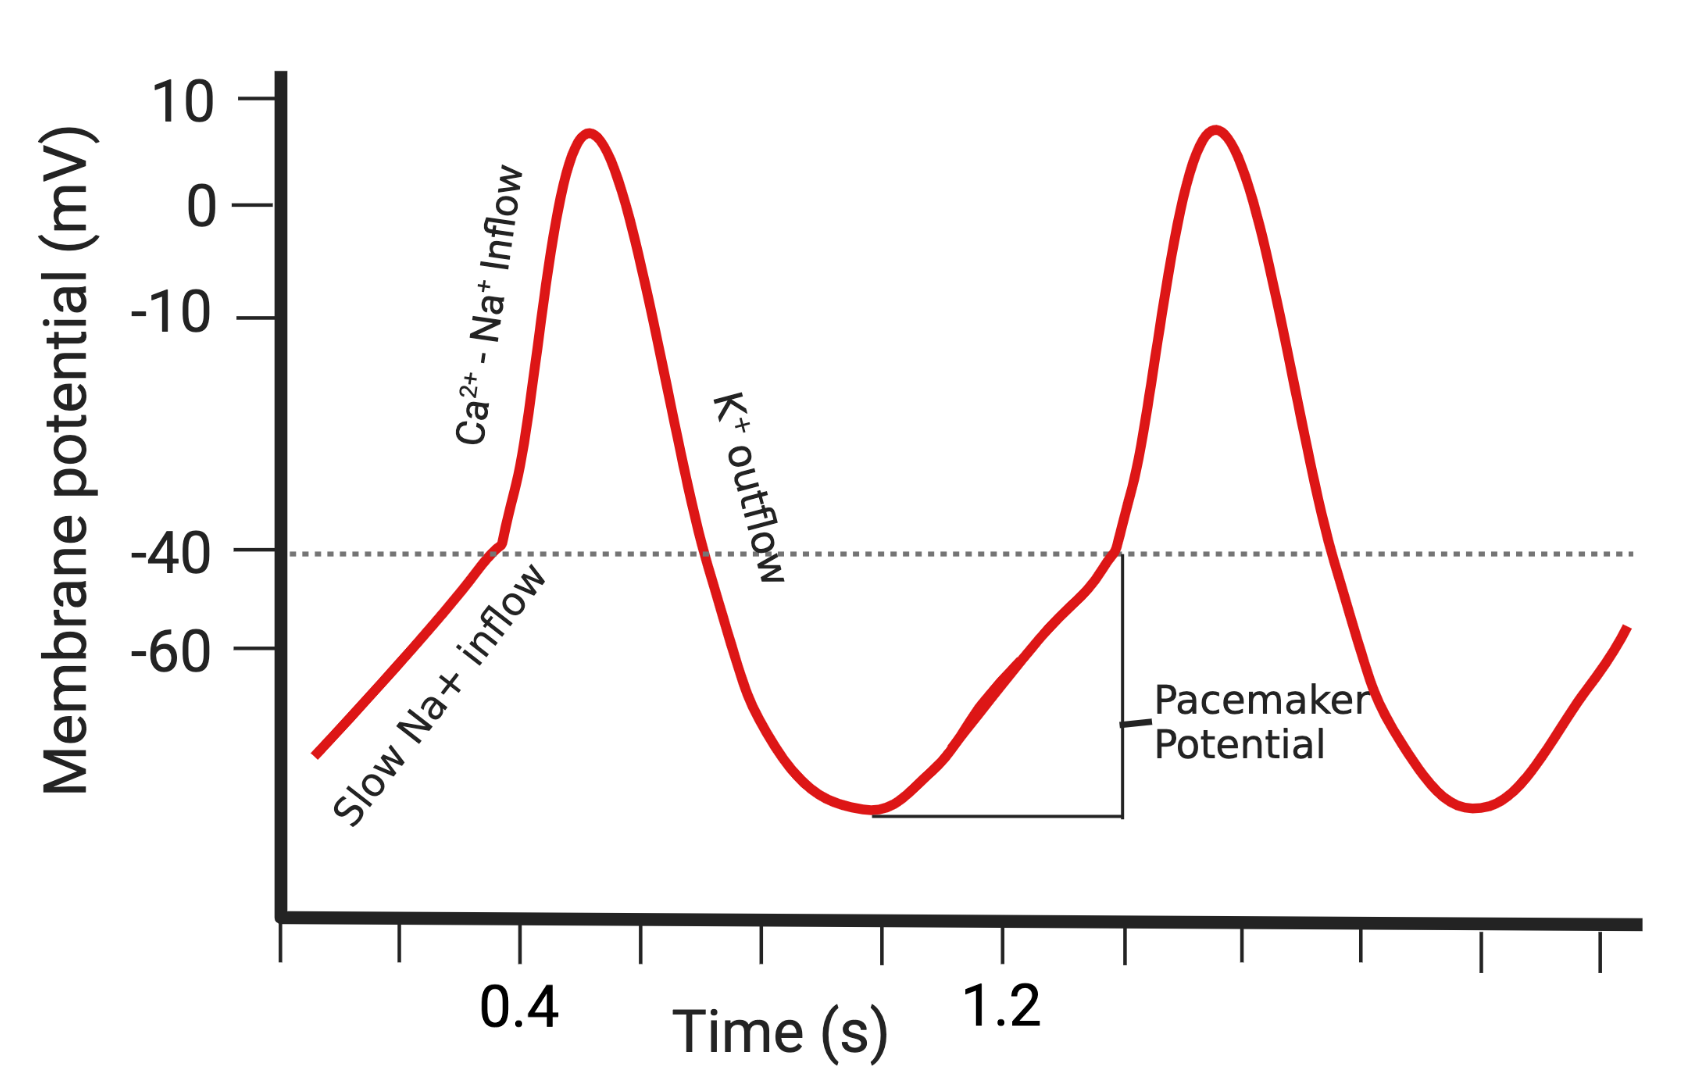
\includegraphics[width=0.5\linewidth]{./figure/Cardiac_SA_Node_AP.png}
    \caption{Cardiac Sino Atrial Node Excitation \footnotesize{(Created with BioRender.com)}}
    \label{fig:Cardiac_SA_Node_AP}
\end{figure}

\subsubsection{Conductivity} 

An excitation of the SA node results in full excitation of all the cardiac muscle cells, first in the atria and after a delay, in the ventricles. There are three features of the myocardium that lead to this pattern of conductivity. 

\begin{figure}[!h]
    \centering
    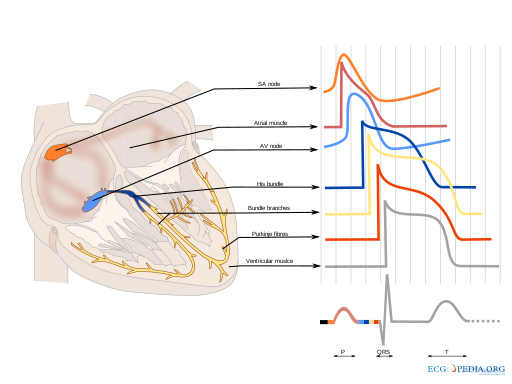
\includegraphics[width=.5\linewidth]{./figure/Cardiac_Conduction.png}
    \caption{Cardiac Conduction \& Shapes of Excitation \footnotesize{(Created with BioRender.com)}}
    \label{fig:Cardiac_Conduction}
\end{figure}

\begin{enumerate}
    \item There are specialized cardiac cells that form a conduction network (See Figure \ref{fig:Cardiac_Conduction}. The conduction network starts with the SA node sending a wave of excitation through the atria, facilitated by intra-nodal fibers (not shown in Figure \ref{fig:Cardiac_Conduction}) that can rapidly carry an excitation from the SA node to the atrio-ventricular (AV) node. The excitation through the atria results in the P wave of the electrocardiograph (ECG). The excitation of the AV node and its distal conduction component, the bundle of His, is slower and delays the excitation of the ventricles (the PR interval on the ECG). Once through the AV node and bundle of His the excitation travels rapidly down the right and left bundle branches to the purkinje fibers. The branching conduction network in the ventricles is critically important to rapid and synchronous excitation of the ventricles (the QRS complex in the ECG). Atrial repolarization is a minor event and is easily lost in the waves of the QRS. Ventricular repolarization is a more substantial event because the ventricles are more substantial muscles and results first in a return to baseline (ST segment on the ECG), and then the T wave on the ECG. It should be noted in Figure \ref{fig:Cardiac_Conduction} that the AV node fibers have a pacemaker potential but it is smaller than the SA node pacemaker potential. The SA node is the pacemaker under normal circumstances because it has a larger pacemaker potential and reaches the excitation threshold earlier than the AV node. However, if the SA node fails, the AV node reaches the excitation threshold and initiates ventricular excitation.
    \item There is a fibrous connective tissue boundary between the atria and the ventricles that does not transmit an excitation (does not have an excitable membrane). This helps ensure that ventricular excitation occurs only through excitation of the AV node (and no other way). The AV node ensures that the ventricular contraction occurs after a delay so that there is time for atrial contraction to push the final 20-30\% of blood into the ventricles for the final stretch of the ventricles which facilitates more tension, thus more pressure for circulation. The "atrial kick" as this is referred facilitates greater tension and thus pressure during ventricular contraction.
    \item Each excitation travels from cardiac muscle fiber to the surrounding cardiac muscle fibers due to the presence of intercalated discs that have gap junctions between cardiac muscle fibers (See Figure \ref{fig:Cardiac_Gap_Junctions}. The presence of these gap junctions not only allows, but greatly expedites, the excitation of one fiber to the next. This is fundamentally different from skeletal muscle where each muscle fiber is insulated from nearby muscle fibers by the endomysium. In skeletal muscle this fiber to fiber excitation would be deleterious to controlled, coordinated movement. But in cardiac muscle the fiber to fiber wave of excitation facilitates a synchronized contraction of all atrial, and then ventricular fibers. Such "all together" contraction facilitates the change in atrial and ventricular chamber size which facilitates the change in pressure necessary for circulation.
\end{enumerate}

\begin{figure}[!h]
    \centering
    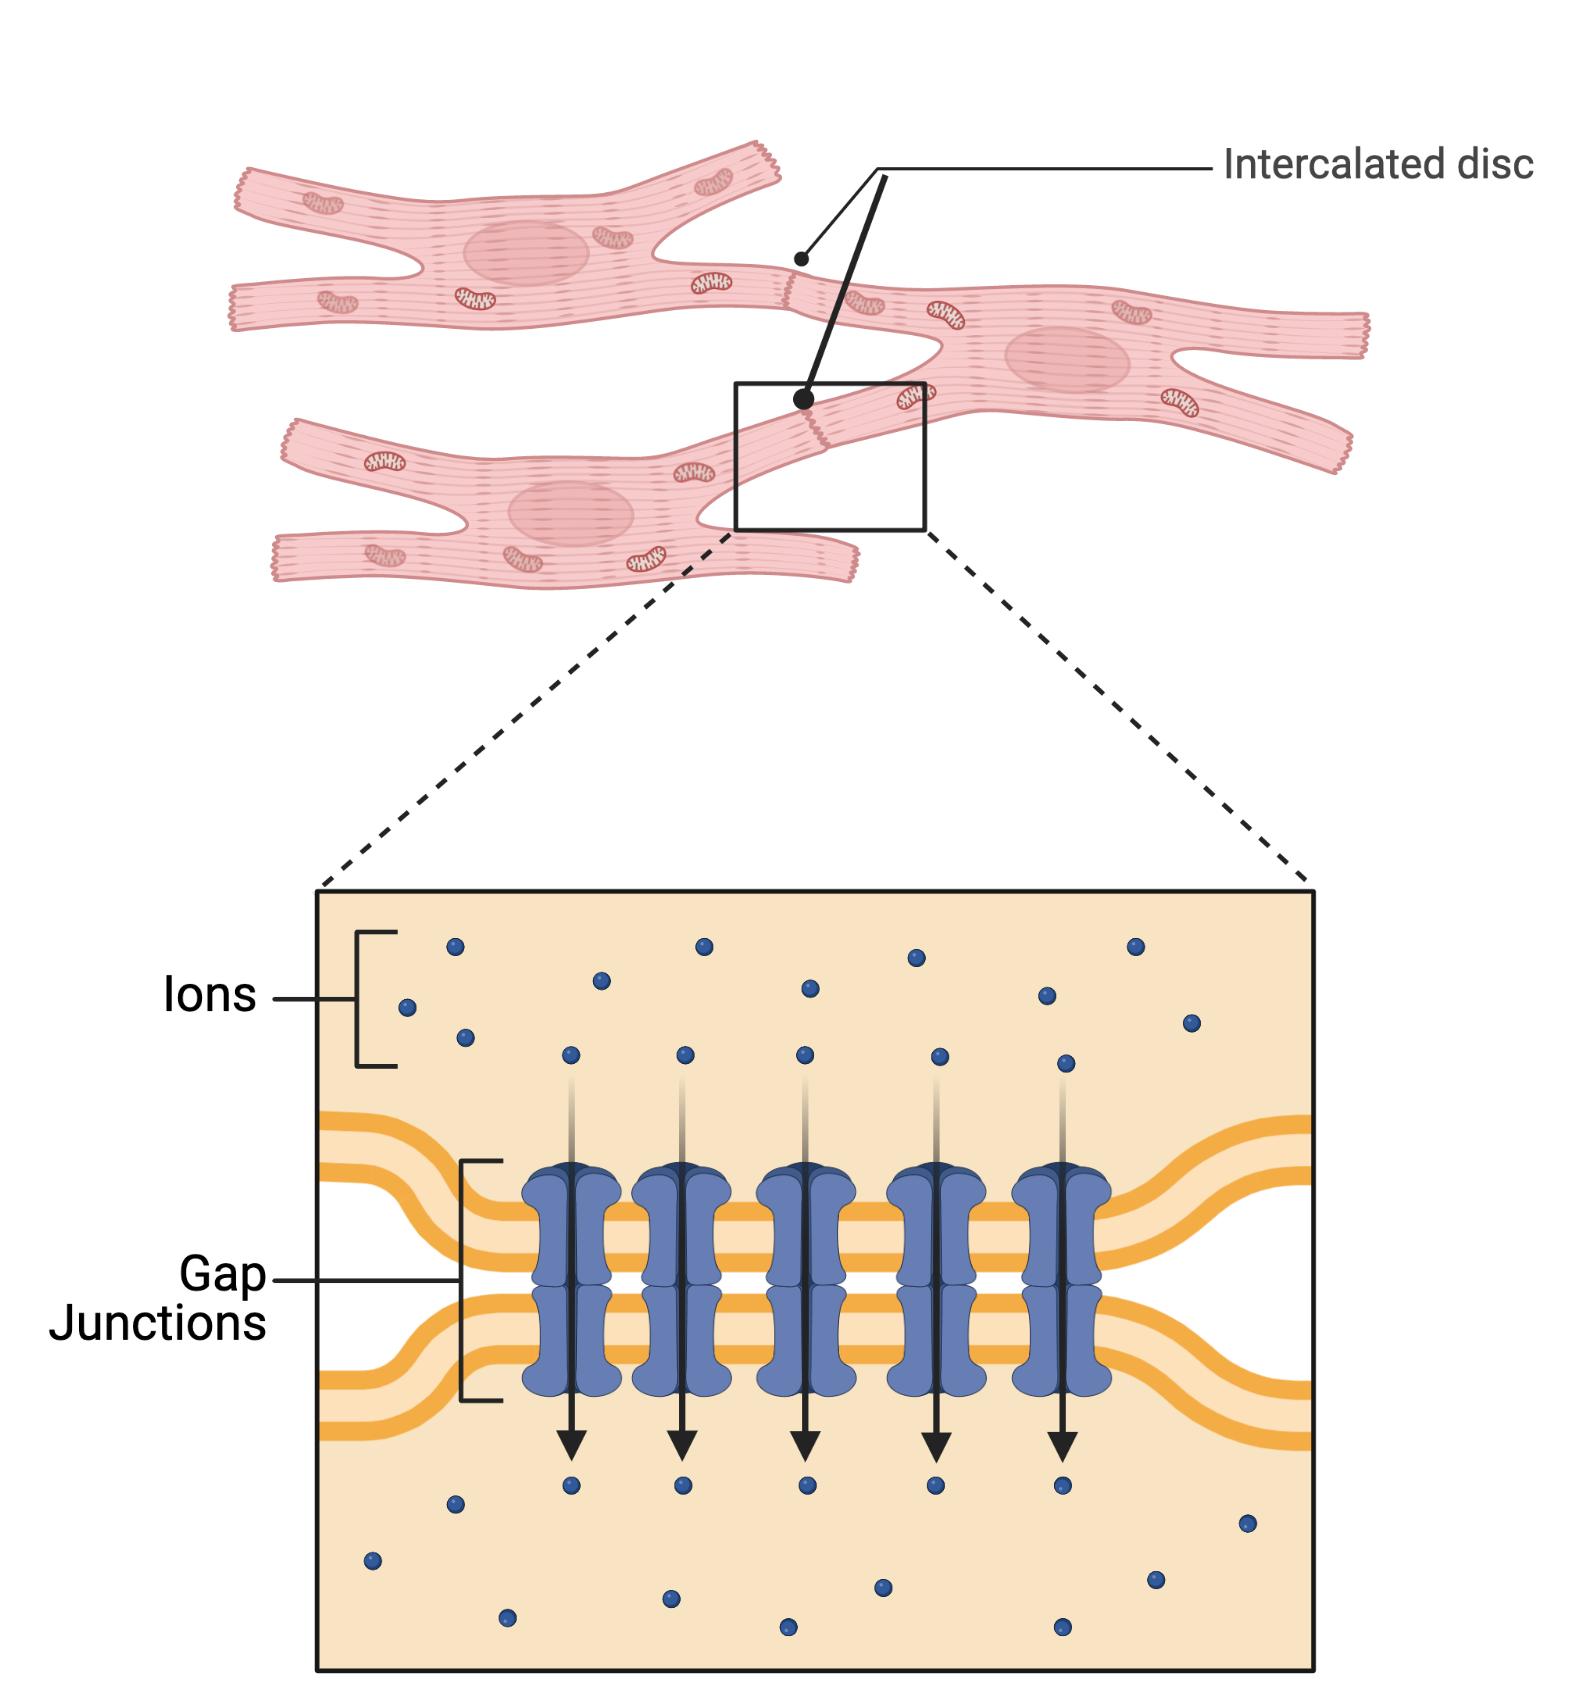
\includegraphics[width=0.5\linewidth]{./figure/Cardiac_Gap_Junctions.png}
    \caption{Intercalated Discs with Gap Junctions \footnotesize{(Created with BioRender.com)}}
    \label{fig:Cardiac_Gap_Junctions}
\end{figure}

\paragraph{Electrocardiogram (ECG)}

The wave of excitation through the cardiac conduction pathway and cardiac muscle fibers generates enough electrical potential to be measured by electrodes on the skin surface. There are several possible electrode placement arrangements, the most popular being referred to as a 12-lead ECG. The 12-lead ECG requires 10 electrodes. Four electrodes are on (or near) the limbs (six limb leads), and six electrodes are on the thorax and surround the heart (six precordial leads). Lead II arises from electrodes on the right arm and left leg and tracks the wave of excitation in the frontal plane from the SA node (origin) through the left ventricle. The ECG wave from Lead II is the most commonly depicted ECG wave. Precordial ECG waveforms that are similar to Lead II include V4, V5 and V6.  Lead II, V4, V5 and V6 are commonly utilized for routine ECG monitoring for arrhythmias. 

A normal ECG is said to display sinus rhythm (sinus referring to the SA node). Figure \ref{fig:ECG} displays the sinus rhythm waves from a normal ECG from a single cardiac cycle from the view of Lead II. Readers are encouraged to view videos of ECG in real time as a preferred approach to becoming familiar with rhythm analysis. A video of normal sinus rhythm is available at this \href{https://youtu.be/Q0JMfIVaDUE?list=PLNN6HI4OXQmyOMNWWrQCCQP559lvbcy4b}{link.} Another option for practicing ECG rhythm analysis is available on iOS and Android devices is the \href{https://simplsim.com/}{Simpl-Simulated Patient Monitor}.

\begin{figure}[!h]
    \centering
    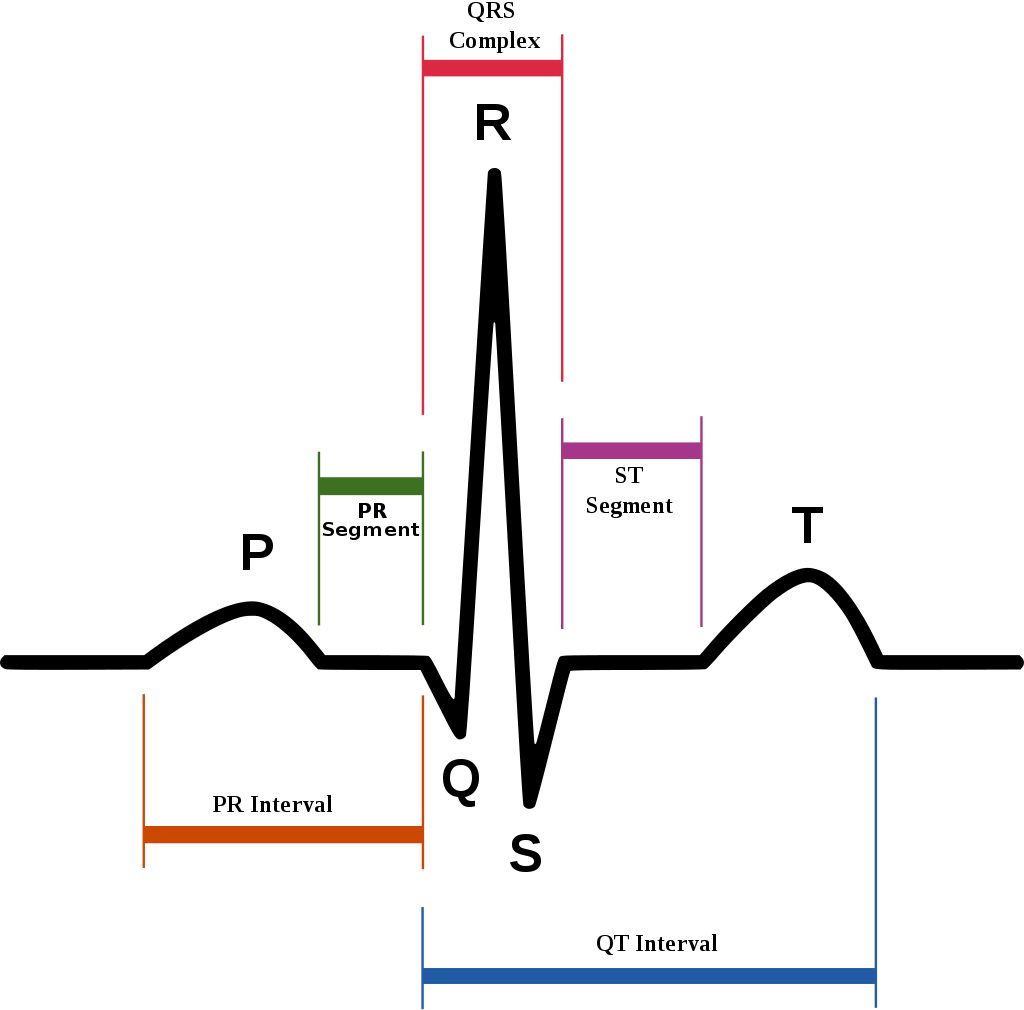
\includegraphics[width=0.5\linewidth]{./figure/ECG.png}
    \caption{ECG Waves (Lead II) \footnotesize{(From Wikipedia  \href{https://commons.wikimedia.org/wiki/File:SinusRhythmLabels.svg}{Sinus Rhythm Labels}, CC BY-SA 4.0)}}
    \label{fig:ECG}
\end{figure}

Table \ref{table:ECGWaves} refers to Figure \ref{fig:ECG} and provides further insight into the excitation event and clinical significance of each wave, segment and interval. ECG abnormalities that must be recognized during real time, single lead rhythm analysis are discussed later in the chapter under practice considerations.

\begin{table}[h!]
\centering
\begin{tabular}{||c c c ||} 
 \hline
 ECG & Excitation Event & Significance \\ [0.5ex] 
 \hline\hline
 P Wave & Atrial Depolarization & SA node, atria \\ 
 PR Segment & AV node delay & AV Node  \\
  PR Interval & SA \& AV node & SA \& AV node  \\
 QRS Complex & Ventricular Depolarization & Ventricles, RR Interval inversely proportional to HR  \\
 ST Segment & Ventricular Repolarization & Ischemia, Injury  \\
 QT Interval & Ventricular De + Repolarization & Long QT syndrome  \\ 
 T Wave & Ventricular Repolarization & Infarction \\ [1ex] 
 \hline
\end{tabular}
\caption{ECG Waves, Segments, Intervals and their excitation events and significance}
\label{table:ECGWaves}
\end{table}


\subsubsection{Contractility}

An excitation results in full tetany of the myocardium and generates enough tension to generate enough pressure for circulation. For a single excitation to result in full contraction of the atria and then the ventricles requires enough $Ca^{2+}$ to be released with one excitation for tetany (not just a twitch). There are two related features that allow for this to occur in cardiac muscle. 

\begin{enumerate}
    \item The cardiac muscle excitation (action potential) is prolonged (See Figure \ref{fig:Cardiac_Ventricular_AP}). It is prolonged due to specialized voltage gated $Ca^{2+}$ channels that allow an inward movement of $Ca^{2+}$ beyond the initiation of the excitation by $Na^+$. The prolonged excitation occurs all the way down to the SR which continues to release $Ca^{2+}$. 
    \item Prolonged SR release of $Ca^{2+}$ into the cell also contributes to the prolonged excitation of the membrane itself (a positive feedback system).
\end{enumerate}

\begin{figure}[!h]
    \centering
    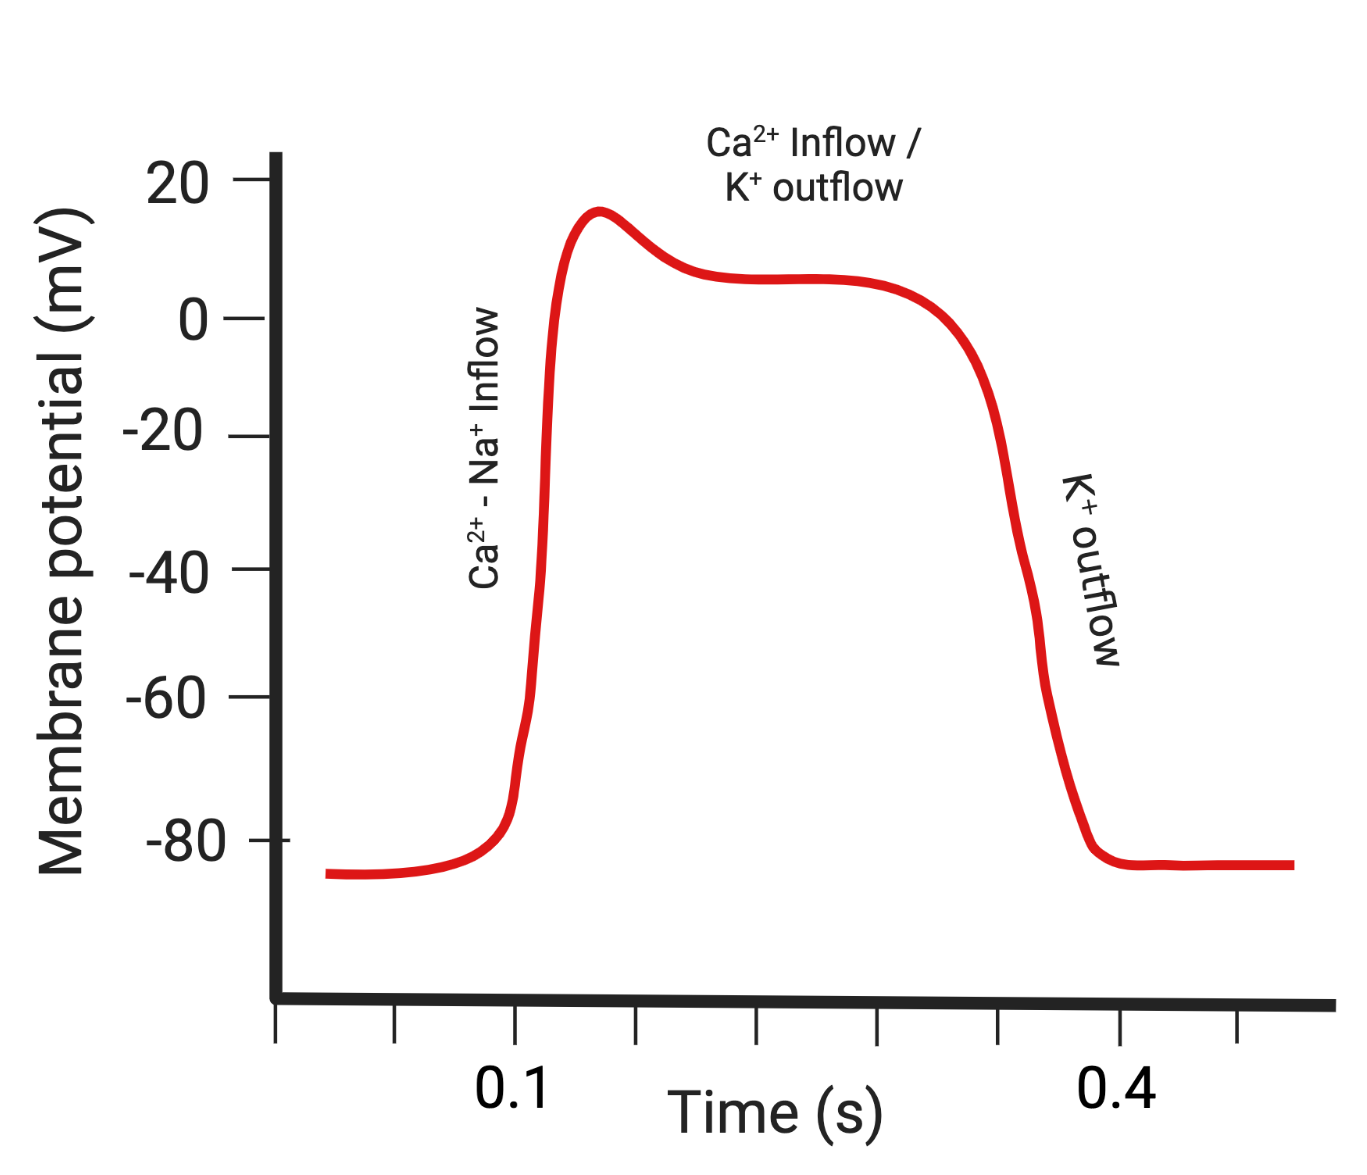
\includegraphics[width=0.5\linewidth]{./figure/Cardiac_Ventricular_AP.png}
    \caption{Ventricular Excitation \footnotesize{(Created with BioRender.com)}}
    \label{fig:Cardiac_Ventricular_AP}
\end{figure}

The primary take away message is that an excitation of a cardiac muscle fiber is prolonged due to inward movement of $Ca^{2+}$ across the sarcolemma, which leads to prolonged SR release of $Ca^{2+}$ for activation that also promotes prolonged excitation. 

\begin{warning}{Cardiac $Ca^{2+}$ Pharmacological Targets}
    Based on the importance of $Ca^{2+}$ in both prolonged excitation and activation of cardiac muscle fibers it is not surprising that medications influencing $Ca^{2+}$ make up two major classes of cardiovascular medications. $Ca^{2+}$-channel blockers decrease the influx from the membrane (anti-arrhythmic) or the SR (anti-hypertensive); and digitalis, which increases the presence of $Ca^{2+}$ in the cardiac muscle fiber.
\end{warning}

\subsection{Regulation}

The regulation of cardiac muscle tension, as part of cardiac pump function (or just cardiac function) is involved in the regulation of $\dot{Q}$. Regulatory mechanisms can vary cardiac pump rate (HR) and vary is contractility (amount of tension and therefore pressure). 

Equations \ref{eq:Q_HRSV} and \ref{eq:SV} are useful models when connecting the regulation of cardiac muscle pump function to $\dot{Q}$. Combining these equations by substituting SV with its components from Equation \ref{eq:SV} results in:

\begin{equation}
    \dot{Q} = HR \times EDV \times LVEF
    \label{eq:Q_HREDVEF}
\end{equation}

\begin{question}{If interested let me know}
    I have a note to myself to make a graphic on the regulation of cardiac function that integrates the past few pages but I don't have the time to do this for this draft. But if anyone does this while studying and is interested in payment for your artwork (if accepted of course), let me know. You'd also get credit for your work in the caption of the figure.
\end{question}

Based on Equation \ref{eq:Q_HREDVEF} there are two ways for cardiac pump function to regulate $\dot{Q}$. As previously discussed the regulation of $\dot{Q}$ results in changes to BP which is regularly monitored to provide feedback.

\begin{enumerate}
    \item Regulate heart rate (HR) - referred to as chronotropy
    \item Regulate tension (contractility) (LVEF) - referred to as inotropy
\end{enumerate}

Equation \ref{eq:Q_HREDVEF} also includes the possibility of using venous return to regulate cardiac pump function. However, venous return is only minimally regulated. Venous return and its EDV are a consequence of venous circulation pressures which are largely determined by skeletal muscle activity. There are changes to vascular tone, but due to the small amount of muscle in the walls of the veins there is much less capacity to regulate venous tone than arterial tone. 

\subsubsection{Neuroendocrine Influence of the Cardiac Pump}

\paragraph{Neural Input}

The autonomic neuroendocrine system influences the heart via direct neural connections and through circulating hormones. It is important to keep in mind that the SA node is the pacemaker. The neuroendocrine input influences, but does not pace, the heart. The multitude of competing external influences to the pacing of HR is one of the reasons for the phenomenon known as HR variability (HRV). 

The parasympathetic (cholinergic) system has direct neural input through the cardiac branch of the vagal nerve (Cranial Nerve X). Vagal nerve activity generally decelerates cardiac function, thus decreasing HR, speed of the conduction wave of excitation and to a lesser extent contractility. The right vagus nerve stimulates primarily the SA node and affects rate, whereas the left vagus nerve stimulates primarily the AV node and affects AV conduction. Note that parasympathetic neural input does not influence EDV. However, EDV can influence parasympathetic neural input (see the Bainbridge reflex below).

Sympathetic (adrenergic) system neural input is through the thoracolumbar sympathetic system and increases HR and augments contractility, thus increasing cardiac function. 

\paragraph{Endocrine Input}
In response to physical activity or stress, the sympathetic nervous system releases catecholamines (epinephrine and norepinephrine) from the adrenal cortex of the adrenal glands which increases HR and contractility. The endocrine influence of the sympathetic nervous system provides a more efficient mechanism for fight/flight signaling since hormones, once circulating in the blood, continue to exert their influence. 

\subsubsection{Cardiac Reflexes}
Cardiac reflexes influence HR and contractility and can be divided into four general categories: baroreflex (pressure) which was discussed in Chapter \ref{chp:circulation}, Bainbridge reflex (stretch), chemoreflex (chemical reflex), ergoreflex (ergoreceptors). 

\paragraph{Bainbridge Reflex}

Mechanoreceptors located in the right atrial myocardium respond to stretch induced by venous return (EDV). An increased volume in the right atrium results in an increased stretch of the atrial wall. This reflex, known as the Bainbridge reflex, stimulates the vasomotor center of the medulla, which, in turn, increases sympathetic input, and decreases parasympathetic input for an overall increased HR and contractility. Respiratory sinus arrhythmia, an increased HR during inspiration and decreased HR during expiration, may be facilitated by changes in venous return and SV caused by changes in thoracic pressure induced by the respiratory cycle. At the beginning of inspiration when thoracic pressure is decreased, venous return and EDV is greater; therefore a greater stretch is exerted on the atrial wall.

\paragraph{Chemoreflexes}
Chemoreceptors located on the carotid and aortic bodies have a primary effect on increasing rate and depth of ventilation in response to $CO_2$ levels, but they also have a cardiac effect. Increased $CO_2$ tends to promote a higher HR and decreased $CO_2$ a lower HR. However, compared to other reflexes and competing influences over HR the chemoreflexes exert a relatively minor influence.

\paragraph{Ergoreflexes}
Ergoreceptors and the ergoreflex regulates circulation through activation of mechanosensitive afferents to inhibit the sustained vagal effects on the heart caused by an increase blood pressure triggering the baroreflex during physical activity that would otherwise work against the overall need for more circulation.


\subsection{Energetics}

Cardiac muscle is exceptionally well developed for aerobic metabolism, even more so than slow oxidative (SO) skeletal muscle fibers. Even during high intensity exercise cardiac muscle is capable of taking in lactate that is circulating in the blood and facilitating its transformation back into pyruvate and acetyl-CoA for entry into the citric acid cycle (TCA). Only when there is a lack of $O_2$ available for electron transport (ETC) do the aerobic energetic pathways not keep up with glycolosis in cardiac muscle cells (there is no normal anaerobic threshold for cardiac muscle). 

Cardiac muscle is so developed for aerobic metabolism that even at rest the myocardium utilizes approximately 80\% of the $O_2$ delivered the blood. Skeletal muscle, at rest, only utilizes approximately 20\% of the $O_2$ that is delivered in the blood. Though much of this difference is based on the difference in resting metabolic need. This makes cardiac muscle critically dependent on increases in circulation to provide the additional $O_2$ needed in response to increased myocardial oxygen demand (RPP).

\begin{warning}{Rate Pressure Product}
    The rate pressure product (RPP), also referred to as the double product, is described by the equation: $RPP = HR \times SBP$, where HR is heart rate and SBP is systolic blood pressure. It is an indication of cardiac muscle (myocardium) oxygen demand. This experimental observation has useful clinical application. It also demonstrates the fact that pressure generated by the myocardium includes active tension which requires oxygen.
    
    In situations with increased afterload the myocardium must develop more pressure for circulation. This greater pressure requires greater tension. This greater tension requires more ATP. More ATP requires more $O_2$. The more frequently the tension is generated (HR) the more ATP and subsequently $O_2$ is required. The experimental association between RPP and myocardial $O_2$ demand is a rather simple consequence of the underlying relationship between pressure (resistance), active tension and ATP.
    
    If a patient undergoes maximal exercise testing and has myocardial ischemia, RPP can be calculated at the point when ischemia is occurring to establish the patient’s ischemic threshold. RPP at the ischemic threshold can then be used during exercise to provide a safe guideline of exercise intensity. This value is useful even if the patient is on a beta-adrenergic antagonist ($\beta$-blocker). Even though the $\beta$-blocker reduces the HR response by blocking the action of epinephrine and norepinephrine on the heart, it is this mechanism that reduces the risk of reaching ischemia. While on a $\beta$-blocker, HR is not a good linear indication of overall aerobic workload (it loses its linear relationship with $\dot{V}O_2$), the RPP is a good discrete indicator of whether a patient is above or below their ischemic threshold. A patient that starts taking a $\beta$-blocker (adrenergic antagonist) will have a harder time exceeding the ischemic threshold, which is the point of being on a $\beta$-blocker for people with ischemic cardiac disease. 
\end{warning}

\begin{comment}

\begin{backgroundinformation}{RPP Example}
    For example: If HR and SBP at rest are 60 beats per minute (bpm) and 110 mmHg then RPP is 6,600. If these values reach 180 bpm and 200 mmHg for an RPP of 36,000 there is a roughly a 5.5 fold increase in myocardial oxygen demand. To meet that demand a roughly 5 fold increase in myocardial circulation (perfusion) must be achieved. This estimate is most accurate if these values are reached at rest (rare). If these values are achieved during exercise they are a small over estimate of the actual myocardial oxygen demand. During exercise there is a significant increase in the skeletal muscle pumping action on venous circulation. Therefore there is a significant increase in venous return. Increased venous return increases preload. Increased preload increases the contribution of passive tension on cardiac contraction. The increased contribution of passive tension on cardiac contraction reduces the myocardial oxygen demand. 
    Therefore, a HR of 180 and SBP of 200 at rest has a higher myocardial oxygen demand than a HR of 180 and SBP of 200 during exercise despite the same RPP because of the contribution of preload and passive tension to cardiac contractility.
\end{backgroundinformation}
\end{comment}

\subsubsection{Cardiac Circulation}

The major coronary arteries include the left coronary (LCA) which quickly branches into the left anterior descending (LAD) and left circumflex (LCx); and the right coronary artery RCA) (See Figure \ref{fig:Cardiac_Circulation}). LAD distributes the anterior wall of both ventricles (L > R) including the septum. LCx the left lateral and posterior walls. LAD and LCx join for distribution in the inferior myocardium. RCA distributes to the anterolateral, lateral, posterior and inferior RV. The RCA and LCA are the first two vessels off of the aorta. Blood is pumped to these large superficial coronary arteries during ventricular systole. At this time, myocardial contraction limits the flow of blood to the myocardium; therefore myocardial tissue is perfused during diastole.

\begin{figure}[!h]
    \centering
    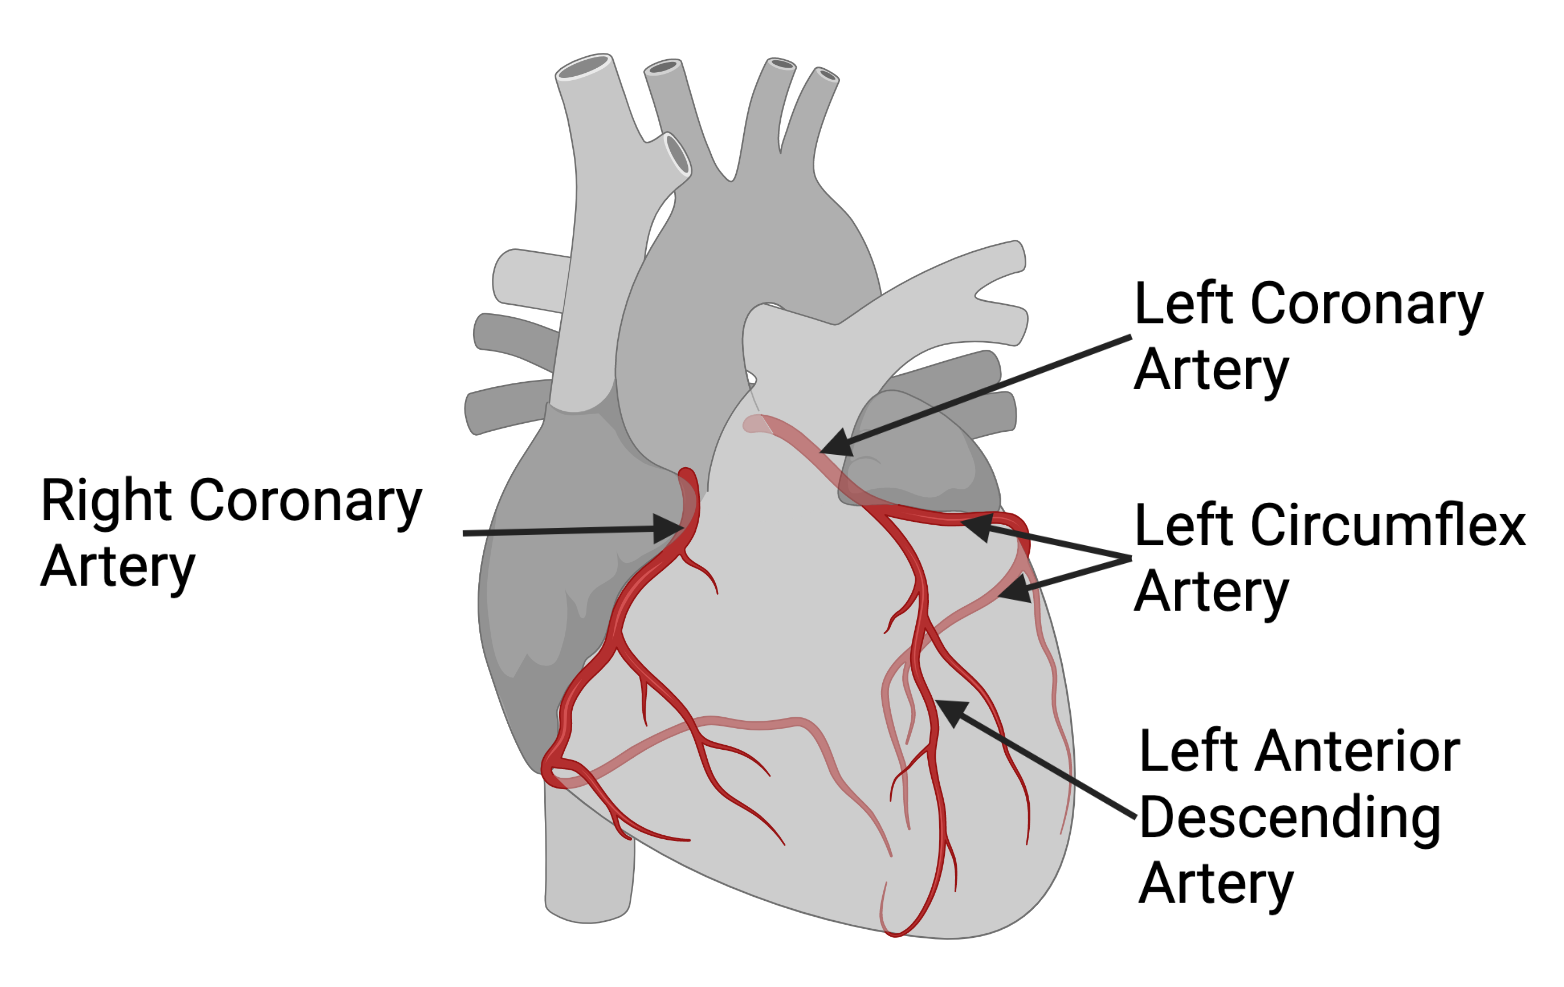
\includegraphics[width=0.5\linewidth]{./figure/Cardiac_Circulation.png}
    \caption{Cardiac Circulation \footnotesize{(Created with BioRender.com)}}
    \label{fig:Cardiac_Circulation}
\end{figure}



\section{Cardiac Cycle}

The events of the cardiac cycle are displayed in Figure \ref{fig:Cardiac_Wiggers}. 
\begin{figure}[!h]
    \centering
    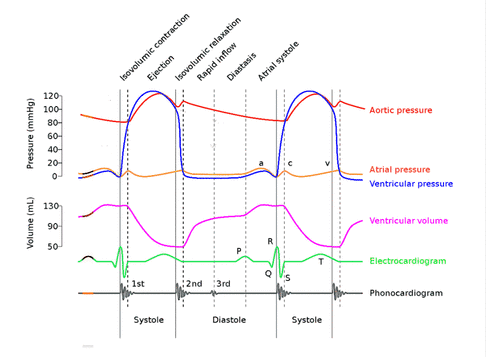
\includegraphics[width=.75\linewidth]{./figure/Cardiac_Wiggers.png}
    \caption{Wiggers Diagram of the Cardiac Cycle \footnotesize{(From Wikipedia  \href{https://en.wikipedia.org/wiki/Wiggers_diagram}{Wiggers Diagram Entry}, CC BY-SA 4.0)}}
    \label{fig:Cardiac_Wiggers}
\end{figure}

Circulation throughout the cardiac cycle depends on circulatory and cardiac pressure gradients. The right side of the heart is a low-pressure system with little vascular resistance in the pulmonary arteries, whereas the left side of the heart is a high-pressure system with high vascular resistance from the systemic circulation. The cardiac cycle is the period from the beginning of one contraction, starting with SA node depolarization, to the beginning of the next contraction. Systole is the period of contraction, and diastole is the period of relaxation. Systole and diastole can also be categorized into atrial and ventricular components.

\begin{itemize}
    \item Atrial diastole is the period of atrial filling. The flow of blood is directed by the higher pressure in the venous circulatory system.
    \item Atrial systole is the period of atrial emptying and contraction. Initial emptying of approximately 70\% of blood occurs as a result of the initial pressure gradient between the atria and the ventricles. Atrial contraction then follows, squeezing out the remaining 30\%. This is commonly referred to as the atrial kick.
    \item Ventricular diastole is the period of ventricular filling. It initially occurs with ease; then, as the ventricle is filled, atrial contraction is necessary to squeeze the remaining blood volume into the ventricle. The amount of stretch placed on the ventricular walls during diastole, referred to as left ventricular end diastolic pressure (LVEDP), influences the force of contraction during systole.
    \item Ventricular systole is the period of ventricular contraction. The initial contraction is isovolumic (i.e., it does not eject blood), which generates the pressure necessary to serve as the catalyst for rapid ejection of ventricular blood. The left ventricular ejection fraction (EF) represents the percent of end diastolic volume ejected during systole and is normally approximately 60\%.
\end{itemize}

\paragraph{Understanding Wiggers Diagram}

Understanding the cyclic events of Wiggers Diagram in Figure \ref{fig:Cardiac_Wiggers} requires an understanding of pressure changes due to volume and volume changes due to pressure. Readers should start from the left and track the changes in each wave, using the ECG as a guide to the excitation events. Once the reader understands each wave they should proceed to observing the coherence between two, then three and finally all of the waves through the two cardiac cycles depicted. An understanding of cardiac function and the cardiac cycle can be confirmed when Figure \ref{fig:Cardiac_Wiggers} can be reproduced based on an understanding of the events (not by memorizing how to reproduce it). Though, some individuals find that learning to reproduce it by memorizing it ultimately leads to an understanding of cardiac function.


\section{ECG Rhythm Analysis}

ECG rhythm analysis allows identification of minor through major cardiac arrhythmias (conduction abnormalities) as well as deviations in wave forms that are associated with ischemia, injury or infarction of the myocardium (myocardial circulation abnormalities). 

Rhythm analysis includes the observation of one ECG lead in real time via a hard wired ECG monitor or a telemetry (wireless) ECG monitor. The first question when observing an ECG is whether it appears normal, that is with all of its waves and segments in order and spaced as expected. A general approach when observing the ECG in real time is to ask:

\begin{itemize}
    \item Is every P wave followed by a QRS?
    \item Is every QRS preceded by a P wave?
    \item Is every QRS followed by a T wave?
    \item Is every T wave preceded by a QRS?
    \item Is every T wave followed by a P wave?
    \item Is every P wave preceded by a T wave?
    \item Is the PR segment normal width?
    \item Is the QRS complex normal width?
    \item Does the ST segment quickly return to baseline?
    \item Are the QRS complexes reasonably and regularly spaced (RR Intervals)?
\end{itemize}


\subsubsection{Arrhythmias}

Examination for arrythmias can occur with any ECG lead (any one of the standard 12, or other less commonly used electrode and lead configurations). Every lead provides the same information about conduction. For example, if a P wave is missing or a PR interval is long in Lead II, it will be equally missing or as long in Lead aVL or V3 (or any of the other leads). 

\paragraph{Tachyarrythmias (Ectopy)}

Tachyarrythmias refer to arrhythmias associated with more excitation than usual during cardiac conduction. Such aberrant excitation usually results in a higher heart rate. Tachycardia is a HR higher than 100 bpm and is not technically an arrhythmia - though if its occurs without provocation (physical, mental or emotional stress) then it may be indicative cardiac or autonomic dysfunction. When tachycardia is unprovoked it is often referred to as supra-ventricular tachycardia (SVT) or atrial tachycardia. The most common type of SVT is paroxysmal SVT (PSVT). Paroxysmal simply means it comes and goes without any currently understood provocation (cause).
There are a group of tachyarrythmias caused by ectopic action potentials that cause ectopic excitations and beats. Ectopic simply means these excitations are not originating in the SA node and following the normal excitation conduction pathway. Ectopy originates from an ectopic focus (myocardial cells causing an action potential) or if more than one focus, as ectopic foci. An ectopic focus (or foci) can occur due to myocardial cell irritation (producing an excitation when it should not, i.e. caffeine or other stimulants), or due to myocardial cell depression (delay or block in conduction caused by ischemia, injury or scar tissue) that produces a recurrent loop of self perpetuating excitation within the myocardium). 

Table \ref{table:Tachyarrhythmias} organizes six different tachyarrhythmias based on where they occur (atria or ventricles) and the regularity of the ectopic focus (or foci) excitations.

\begin{table}[h!]
\centering
\begin{tabular}{||c c c ||} 
 \hline
   & Atria & Ventricle \\ [0.5ex] 
 \hline\hline
 Occasional Ectopic Focus & Premature Atrial Contr. (PACs) & Premature Ventricular Contr. (PVCs)\footnotemark\footnotetext{Also referred to generally as ventricular ectopy or ventricular premature beats (VPBs)} \\ 
 Occasional Ectopic Foci & PACs & Multifocal PVCs \\
 Non Stop Ectopic Focus & Atrial Flutter (AFlutter)& Ventricular Tachycardia (VTach)  \\
 Non Stop Ectopic Foci & Atrial Fibrillation (AFib) & Ventricular Fibrillation (VFib)  \\ [1ex] 
 \hline
\end{tabular}
\caption{Types of Ectopic Tachyarrhythmia}
\label{table:Tachyarrhythmias}
\end{table}

The severity of all conduction abnormalities is based on the impact they have on cardiac output and blood pressure (hemodynamics). In general the impact a tachyarrhythmia has on hemodynamics is greater proceeding down the rows; and is always greater in the ventricular column than the atrial column. For example, PACs have little, if any, impact on hemodynamics; whereas VFib does not produce any circulation at all so there is no cardiac output and no blood pressure (and therefore no pulse). 

Since the tachyarrhytmias exist on a spectrum, it is required that a physical therapist can identify which tachyarrhytmia is present should one arise (or be part of a patient's chronic condition). For example, it is not appropriate to stop activity due to AFib in a patient with chronic AFib, but it is important to monitor the ventricular rate and BP for signs of worsening hemodynamics in AFib. Nor is it required to stop activity due to PACs or PVCs in all situations. 

A YouTube playlist of tachyarrhythmias is available at this \href{https://www.youtube.com/playlist?list=PLNN6HI4OXQmwFdE8LVIGC_l5WG2ViWAy3}{link.}

\paragraph{Bradyarrythmias \& Blocks}

Bradycardia refers to any HR below 50 bpm. However, like tachycardia, bradycardia does not always indicate there is a conduction problem. Whether bradycardia is a problem comes down to whether it is creating problems with hemodynamics. Generally, if there is an abnormality causing bradycardia it will provoke problematic changes in hemodynamics, for example, sick sinus syndrome or third degree AV block. A normal cause of bradycardia that does not provoke problematic changes in hemodynamics is being well conditioning from exercise training.

Bradyarrhythmias can be caused by AV blocks, though not all instances of AV blocks create bradycardia. It is just common to classify blocks as a bradyarrhythmia. There are three degrees of AV Block, and four types (there are two types of second degree AV block).

\begin{itemize}
    \item First Degree AV Block: Prolonged PR Interval
    \item Second Degree AV Block - Mobitz 1 (Wenkebach) - progressive prolongation of the PR interval until finally there is a P wave without a QRS indicating the conduction was blocked which is then followed by a normal PR interval that begins progressive prolongation (this pattern repeats)
    \item Second Degree AV Block - Mobitz 2 - normal PR interval with an occasional P wave with no QRS
    \item Third Degree AV Block - complete AV block (also referred to as complete heart block) P waves and aberrant looking QRS complexes are completely dissociated (though may occasionally align so identification requires watching the ECG for several cycles)
\end{itemize}

A YouTube playlist of bradyarrhythmias and AV blocks is available at this \href{https://www.youtube.com/playlist?list=PLNN6HI4OXQmyt5Ql2um3MthEtLkdJnywd}{link.}

The severity of AV blocks is related to the impact they have hemodynamics. As can be expected, the severity increases from First Degree to Third Degree. Mobitz 2 is considered more severe to Mobitz 1, not due to hemodynamic differences, but because it is more likely to deteriorate into Third Degree AV block.

\subsection{Myocardial Circulation Abnormalities}

Abnormalities in myocardial circulation (perfusion) such as ischemia lead to hypoxic conditions in the myocardial cells. If the ischemia persists cell death will occur. Prior to cell death an early indication of ischemia includes changes to the ST segment of the ECG. In a very general way, ST changes are indicative of ischemia and/or injury. This more general fact is sometimes made more specific, with ST depression taken as a sign of myocardial ischemia and ST elevation taken as a sign of myocardial injury. Myocardium that is injured may be reversibly injured (will recover) or irreversibly injured (will die, infarction). 

A YouTube playlist of ST segment changes is available at this \href{https://www.youtube.com/playlist?list=PLNN6HI4OXQmyHL-CDiLqrBSkv6E1Vk0cS}{link.}

One of the problems with the more specific claims of ST changes is that it assumes the ECG lead being observed is a lead that has the best view of the myocardium that has ischemia. Unlike the the arrhythmias which are seen equally well in all ECG leads, a circulation abnormality resulting in ischemia is local to the region of the myocardium with the circulation abnormality (rarely the entire myocardium). For example, aVR tends to have a reversed polarity to Lead II (what goes up in Lead II, goes down in aVR; what goes down in Lead II, goes up in aVR). If ischemia is in an area that Lead II shows depression, it may appear as elevation in aVR. During the diagnostic process (a cardiac stress test) a 12 lead ECG is utilized and additional testing strategies are utilized to confirm that what was observed was in fact ischemia. A cardiologist can get a good idea of where the ischemia is occurring from the 12-lead ECG, which is then confirmed with imaging (nuclear scans or catheterization). When it is known which location (and therefore lead) best pin points the area with a propensity for ischemia then that lead (or a couple of leads) can be utilized for rhythm monitoring. In such situations it is mostly true that ischemia appears as ST depression, and injury appears as ST elevation.

Since the physical therapist using rhythm analysis is primarily interested in identifying abnormalities that warrant the cessation of activity and alerting members of the medical team of such abnormalities (not in making a diagnosis), simply identifying ST changes is sufficient. Both ischemia and injury are sufficient reason to stop activity and alert members of the medical team. In fact, the risk associated with myocardial ischemia and injury is sufficient to warrant extra caution and stopping activity if ST changes are suspected while observing the ECG rhythm. In other words, if the ST segment appears above or below the baseline its safer to assume it is than to assume it isn't. Cease activity and continue monitoring. As with any such signs, noting other signs and symptoms is warranted (shortness of breath, diaphoresis, chest pain, blood pressure, respiratory rate).

\section{Summary}

The cardiac pump supports circulation. Cardiac muscle includes several characteristics required for its unique role in circulation. Cardiac muscle tension, excitation and regulation support circulation and pressure regulation. Excitation of cardiac muscle can be recorded with the ECG and offers insights into several abnormalities of conduction as well as myocardial ischemia. Monitoring the ECG provide physical therapists with non-invasive insights, that when combined with an understanding of circulatory physiology, provide useful information when working with clients both with and without conditions that directly affect the circulation.

\subsection{Next Step}

With an understanding of mass balance and circulation we can now proceed to the mass balance of oxygen and carbon dioxide in the next two chapters. First we consider Respiration which focuses on gas exchange between the alveoli and blood. Then we turn to Ventilation which focuses on air exchange between the environment and the alveoli (breathing).

\printbibliography[heading=subbibintoc]

\section*{Sample Questions}

\begin{enumerate}
    \item Normal end diastolic volume (EDV) is directly related to normal end diastolic pressure (EDP) and normal ventricular compliance. If a pathology results in reduced ventricular compliance during diastole what would occur?
    \item What myocardium features lead to the normal pattern of myocardial conductivity?
    \item Why is cardiac muscle excitation (action potential) prolonged and what changes to the action potential allow this to occur?
    \item How are options for determining and monitoring ischemic threshold during exercise? 
    \item Which cardiac arrhythmia results in an irregularly irregular pulse rhythm?
\end{enumerate} 
\include{chapter/respiration}
\include{chapter/ventilation}
%\include{chapter/digestion_absorption_metabolism}
%%%%%%%%%%%%%%%%%%%%%%part.tex%%%%%%%%%%%%%%%%%%%%%%%%%%%%%%%%%%
% 
% sample part title
%
% Use this file as a template for your own input.
%
%%%%%%%%%%%%%%%%%%%%%%%% Springer %%%%%%%%%%%%%%%%%%%%%%%%%%

\begin{partbacktext}
\part{Muscle Maintenance, Adaptation, \& Repair}
\noindent 

\end{partbacktext}
%\include{chapter/myostasis}
%\include{chapter/defense}
%\include{chapter/repair}
%%%%%%%%%%%%%%%%%%%%%%part.tex%%%%%%%%%%%%%%%%%%%%%%%%%%%%%%%%%%
% 
% sample part title
%
% Use this file as a template for your own input.
%
%%%%%%%%%%%%%%%%%%%%%%%% Springer %%%%%%%%%%%%%%%%%%%%%%%%%%

\begin{partbacktext}
\part{Integrative Exercises}
\noindent 
% Introduce the integrative exercises 
\end{partbacktext}
%% !TEX root = ../notes_template.tex
\chapter{Fick's Equation}\label{chp:fick_equation}
Updated on \today
\minitoc

% Hi Nathaniel - anything with a % in front of it is a comment and doesn't get compiled as text into the book. Use it as necessary to leave questions for me or reminders for yourself. Also - at the moment this chapter is not added to the compile list. It won't show up in the PDF until I add it to the file called "book.tex". If you want to see how its compiling you could remove the "%" in front of the reference to it in the "book.tex" file and hit recompile.

This chapter introduces Fick's equation as a model to connect the muscle and supporting systems roles in attaining and sustaining activity.

% Just the equation for the sake of having it to copy/paste where ever it is needed in the chapter
\begin{equation}
    \dot{V}O_2 = \dot{Q} \cdot (a-v)O_2
\end{equation}



\vspace{5mm}

\textbf{Objectives include:}
\begin{enumerate}
    \item Define Fick's equation and recognize the relevance 
    \item Review the determinants of cardiac output and how the comprising variables may 
    \item
    \item
    \item
    \item
\end{enumerate}


Fick's equation offers a method to determine substance consumption using a set of known variables: 

\begin{enumerate}
    \item Flow rate to an organ/system
    \item The concentration of substance in the arterial blood entering the organ
    \item The concentration  of substance in the venous blood leaving the organ
\end{enumerate}

Specific to Fick’s equation, the substance in question is most typically oxygen. Thus, the necessary components to calculate and apply Fick’s equation relevant to this area of study are as followed:

\begin{enumerate}
    \item Flow rate to an organ/system (cardiac output)
    \item The concentration of oxygen in the arterial blood entering the organ (arterial oxygen concentration, CaO2)
    \item The concentration  of oxygen in the venous blood leaving the organ (venous oxygen concentration, CvO2)
\end{enumerate}

Using these variables, Fick’s equation can be formatted as:

\begin{equation}
    \dot{V}O_2 = \dot{Q} \cdot (a-v)O_2
\end{equation}

Where: 

\begin{itemize}
    \item VO2 = the amount of oxygen taken up by the system or organ
\end{itemize}
\begin{itemize}
    \item Q = cardiac output
\end{itemize}
\begin{itemize}
    \item avO2 difference = the difference in oxygen concentration between the arterial and venous blood (CaO2 - CvO2)
\end{itemize}

In contrast to determining the VO2 using Fick’s equation, another variation of this equation can be used to determine the cardiac output. A simple rearrangement of the equation would yield:

Q = VO2/ avO2 difference 

\begin{equation}
    \dot{Q} = \dot{V}O_2 / (a-v)O_2
\end{equation}

Fick’s equation can be applied systemically (e.g. determining oxygen consumption of the whole system) or at a more local area of the body. For example, Fick’s equation can be used to calculate oxygen consumption specifically to the myocardium using the following variables: 

MVO2 = CBF x (CaO2 x CvO2) 

\begin{equation}
    \dot{MV}O_2 = \dot{CBF} \cdot (CaO_2)(CvO_2)
\end{equation}

Where:
MVO2 = myocardial oxygen consumption
CBF = coronary blood flow
CaO2 = arterial oxygen content
CVO2 = venous oxygen content

It may seem that in the role of the physical therapist, it is not clinically necessary to establish these values as it does not directly pertain to our intervention and/or examination selection. 

Nevertheless, Fick’s equation offers benefit as it lends an understanding as to how flow rate, oxygen consumption, and the difference in arterial and venous oxygen concentration may change under situations which alter homeostatic conditions. The role of this chapter is to look at the determinants of each of the variables in Fick's equation and to understand the interplay of systems that can influence the variables. 

Oxygen consumption is a highly integrated physiological variable and is ultimately determined by the three variables in the Fick equation: cardiac output, arterial oxygen content, and venous oxygen content. As will be seen later in the chapter, these variables are influenced by a number of factors and are constantly monitored and then subsequently adjusted to maintain the equilibrium of each individual system and the body at large. 


\section{Determinants of Cardiac Output}
To begin, this section of the chapter outlines the determinants of cardiac output and evaluates how they can change under varying physiological circumstances. As described in Chapter 7, cardiac output is defined as the volume of blood pumped out by each ventricle per unit of time (one minute). 

The equation for cardiac output is Q = SV x HR. Stroke volume is the product of the left ventricle ejection fraction (LVEF) and the end diastolic volume (EDV), also known as preload. Therefore, Q = SV x HR can be further broken down into: 
 \begin{equation}
    \dot{Q} = (LVEF \cdot EDV) \cdot HR
\end{equation}

 As such, the main determinants of cardiac output are as follows:
1. Heart Rate
2. Stroke Volume (EDV and LVEF) 

Based on the equation (and under stable conditions, i.e. the other variables do not decrease proportionally), increases in any of the above-mentioned variables (LVEF, EDV, or HR) will result in an increased cardiac output and thus, increased systemic and/or localized blood flow. Similarly, decreases in the aforementioned variables without compensatory changes will lower cardiac output. These concepts will be explored later in the text. 

In order for the heart to impart blood effectively through the systemic vasculature, it is imperative that the above physiological characteristics work synergistically. When this synergy is compromised homeostasis is endangered, and pathology can arise. But it is important to remember that these compensatory systems do not only exist in the presence of pathology, but rather, are constantly monitoring and subsequently adjusting variables to accommodate for the changes in homeostasis. 

\textbf{Integrative Exercise: Brachial Blood Pressure During the Supine to Sit Transfer:}
A common, non-pathological integration of the cardiac output determinants  (Q, HR, SV) is seen every time a non-pathological patient performs a functional transfer, like the transition from supine to sitting. In a supine position blood flow is evenly distributed throughout the body secondary to the lack of gravity related pressure changes. With the transition to a sitting position, the effect of gravity redistributes blood from the upper torso and extremities into the lower body, which can create a transient decrease in stroke volume due an attenuated venous return. To combat the initial decrease in cardiac output the body (via the baroreceptor reflex) will increase heart rate and venous return mechanisms, therefore normalizing the cardiac output. 

We will begin by evaluating how heart rate may influence cardiac output beyond acting as a direct multiplier in the equation. 

\subsection{Heart Rate}
How might changes in heart rate affect cardiac output? Aside from being a direct multiplier in the equation, heart rate can also have a direct effect on stroke volume (the other multiplier in the cardiac output equation). More specifically, changes in heart rate, whether increased (tachycardia) or decreased (bradycardia) can influence the stroke volume through modulation of diastolic filling time and therefore end diastolic volume. In an otherwise uncompensated state, bradycardia will increase cardiac contractility while tachycardia will decrease cardiac contractility - both achieved via the Frank Starling Mechanism.  More specifically, under bradycardic conditions there is a greater amount of time in-between each myocardial contraction for blood to fill into the left ventricle, which increases end diastolic volume and subsequently, stroke volume. Although this is true in isolated conditions, the effect of heart rate on stroke volume must be examined relative to the cardiac conditions currently present. In other words, under homeostatic conditions these variables rarely change without integrated, multi-variable compensations, which can exist under both acute and chronic circumstances.  Factors such as nervous system activity, hormonal influences, underlying medical/health conditions, and metabolic needs all can influence heart rate and subsequently cardiac output. This concept can be explored more broadly in the context of Fick's equation when evaluating the compensatory mechanisms at play when having a patient undergo a bout of aerobic exercise. 

\paragraph{Integrative Exercise: Heart Rate and Progressive Aerobic Exercise: How are the variables in Fick's Equation affected in a patient that is acutely progressing through a bout of aerobic exercise? What are the drivers for an increase in oxygen consumption with this task?}
An example of the interplay between the multipliers in the cardiac output equation can be seen during a graded exercise program. As a patient gradually increases their exercise workload it is expected to see an elevation in heart rate to meet the metabolic demands of the exercising skeletal muscle. In an otherwise uncompensated state this elevation in heart rate would decrease stroke volume secondary to a decreased diastolic filling time. But, due to the complex multi-system response, it is much more likely to see an increase in stroke volume (see Figure 1.). This increase in stroke volume paired with the elevated heart rate creates a net increase in cardiac output that is typical of a patient acutely increasing there physical activity. This simple example highlights that changes to one variable do not occur in isolation. The body is constantly adapting and adjusting variables across all systems to meet the internal requirements (e.g. elevated metabolic needs) from the external demands (e.g. aerobic exercise). 

\begin{figure}
    \centering
    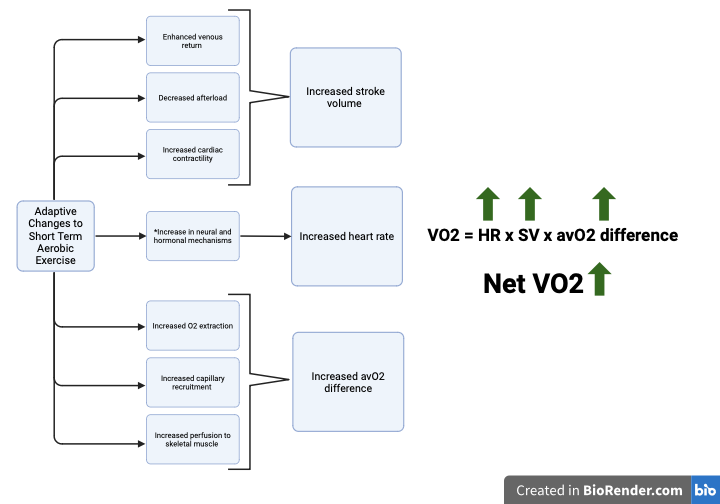
\includegraphics[width=0.5\linewidth]{Short Term Adaptive Changes.png}
    \caption{Figure 1. Short Term Adaptation to Aerobic Exercise}
   \label{fig:enter-label}
   \caption{*Neurohormonal Mechanisms: 
1. Sympathetic activation 
    -Stimulation of cardiovascular control centers in the brain 
2. Parasympathetic withdrawal 
    -Reduced vagal tone 
3. Catecholamine release 
    -Epi, NE 
}
\end{figure} 
As compared to stroke volume, heart rate operates at a wider range of what is generally considered physiologically safe. That is to say, stroke volume tends to remain within a more narrow, well-controlled range. As heart rate is primarily influenced by neural mechanisms (i.e. the response of the autonomic nervous system), this variable can be readily adjusted to accommodate for alterations in homeostasis. As we will look at later in the chapter, stroke volume is predominantly dependent on mechanical factors (e.g. preload, afterload, and contractility), which is unlikely to occur prior to the aforementioned neural response. Heart rate may very well be considered the body's first line of defense in managing changes in cardiovascular homeostasis. 



\begin{figure}



    \centering
    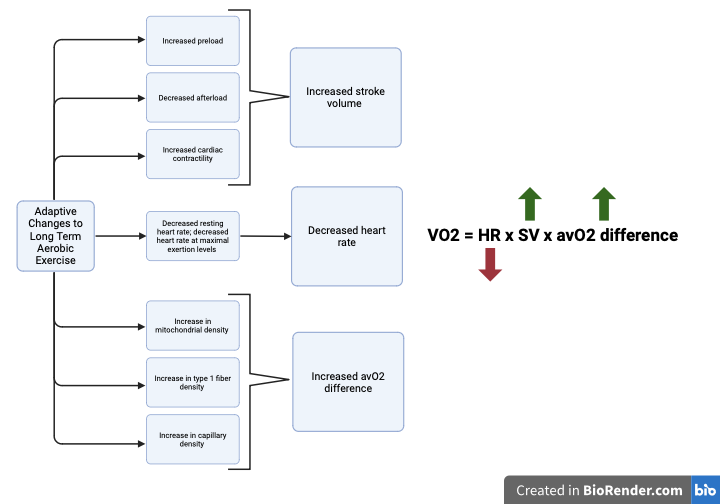
\includegraphics[width=0.5\linewidth]{FicksChronicAerobic.png}
    \caption{Figure 2. Long Term Adaptations to Aerobic Exercise}
    \label{fig:enter-label}
\end{figure}

This acute bout of exercise where all variables in Fick's equation are increased can be compared to the long term adaptive changes seen accompanying a long term aerobic training program. Compared to the integrated cardiac response to acute exercise, long term adaptations result in all variables increasing with the exception of heart rate, which has a net decrease. 

These %Figure 1. --> reasons SV increases when exercising 
Under what situations may bradycardia decrease stroke volume? 
1. Poor ventricular filling time 
2. Poor ventricular contractility 
3. Reduced preload 
4. Increased afterload 
5. Autnomic imbalance 
Under what situations may tachycardia decrease cardiac output?
E.g. Reflex bradycardia with subsequent  hemodynamic instability. 


As we will look at shortly, end diastolic volume is the most important determinant of stroke volume. With this known, heart rate should be recognized as a major determinant in stroke volume and thus cardiac output. Look at the situations below to further explore how fluctuations in heart rate may affect cardiac output. 


and has a significant  as it relates to the body's ability to make an intelligent and efficient offsetting response.

Under what conditions may bradycardia increase stroke volume? 
E.g. Exercise 
1. 



\subsection{Stroke Volume}

Stroke Volume is defined as the volume of blood ejected during one ventricular contraction. 

\begin{equation}
    SV = EDV \cdot LVEF
\end{equation}

The variables of the stroke volume equation (EDV and ESV) are primarily influenced by three variables: 
\begin{itemize}
    \item Preload
    \item Afterload
    \item Contractility
\end{itemize}

Independently, these variables can all increase (or decrease) stroke volume, but often work cooperatively to alter the amount of blood ejected per contraction to ensure physiological needs are attained and sustained. 

First, we will look at these determinants of stroke volume in isolation and then review the interactions between them. 

\subsubsection{\textbf{Preload}} 

Preload is defined as the volume of blood present in the ventricle following the end of the diastolic phase. Fundamentally, the more blood present in the atrium prior to the systolic phase of the cardiac cycle, the higher the stroke volume. They're a number of mechanisms in which preload is shaped including mechanical, neural, hormonal, and  

\paragraph{Increased venous blood volume}
An increased volume of blood present in venous circulation will produce a greater return to the heart resulting in a greater preload, stroke volume, and cardiac output. 

\paragraph{Venoconstriction and rhythmic skeletal muscle contraction}: 
Arteries and veins are innately unique as compared to one another in that veins have valves whereas arteries do not. The purpose of these valves are to prevent back flow. If veins venoconstrict, blood can only move in one direction - forward (moving proximal back to the heart to increase preload and thus, stroke volume). Increasing the internal radius of the veins would only reinforce their role as a reservoir for the blood. 

\paragraph{Atrial kick}: 
Although diastole occurs through primarily passive flow from an area of high pressure (blood filled atria) to low pressure (ventricle), the atrial contraction that occurs at the end of the diastole results in a transient increase in atrial chamber pressure, which creates a greater pressure gradient between the atria and ventricle. This increased pressure gradient results in the further filling of blood left over in the atria that would otherwise be left due to the lack of a large enough pressure gradient.  

\paragraph{Prolonged ventricular diastole}
The prolonging of time in between ventricular diastole allows for an increase in the relaxation phase of the cardiac cycle. This extended relaxation phase allows a greater volume of blood able to enter the ventricle before ventricular contraction. A greater volume of blood prior to the systolic phase means increased preload, increased preload means increased stroke volume.  

\paragraph{Respiratory pump/decreased intrathoracic pressure, increased abdominal pressure (e.g. deep inhalation):} The respiratory pump (diaphragm) can mechanically affect preload by adjusting the influencing the volume inside the thoracic cavity. As the diaphragm contracts it flattens and descends, thereby increasing the volume in the thoracic cavity (decreasing intrathoracic pressure). It is this decrease in intrathoracic pressure that facilitates the expansion and filling of the pulmonary and abdominal veins. 

\textbf{
\subsubsection{Afterload}

Afterload is the pressure that a chamber must overcome to cause blood to flow out of the chamber. Under stable, uncompensated states, afterload has an inversely proportional relationship to stroke volume (i.e. if afterload is increased, stroke volume and thus cardiac output will be decreased). The three primary factors influencing afterload: 
\begin{itemize}
    \item Vessel radius: refer to Poiseuille's Equation 
    \item Arterial compliance (distensibility of arterial vasculature): denoting how the volume of blood within a vessel changes for a given change in pressure.

\begin{equation}
    C = V/P 
\end{equation}
    \begin{itemize}
        \item C = V/P 
        \item Where: 
        \item C = Compliance (mL/mmHg) 
        \item V = Volume (mL) 
        \item P = Pressure 


\textbf{Blood viscosity:} Resistance to blood flow is directly related to the blood viscosity and is related to the friction created by the interaction between the solvent (fluid molecules in the plasma, related solutes (e.g. RBC’s and proteins), and the vessel wall. Increases in blood viscosity will oppose blood flow, which can create changes in hemodynamic stability. In an otherwise unperturbed state, blood viscosity remains a rather stable variable, though can be affected in changes in hematocrit, temperature, and systemic flow. 

\textbf{Arterial Impedance: }
There is an inverse relationship between vessel radius and internal resistance. Atherosclerotic build up results in a reduction in vessel diameter, which increases the pressure required to achieve consistent flow through the vasculature. It is this increase in pressure that reflects an increased afterload. Example: it may be common to find higher arterial pressures in the elderly as the natural aging process creates a reduction of vessel capacitance. At a lower compliance an increased pressure gradient (increased arterial pressure) must be present to maintain consistent flow through the artery. 
    \end{itemize}
    \end{itemize}

\subsubsection{Contractility}

An increase in cardiac contractility will result in an increased stroke volume for a given preload and afterload. This will present as an increased cardiac ejection fraction as a larger proportion of the given end diastolic volume will be ejected from the ventricle due to the increased pressure gradient created by the increased cardiac contractility. 

Factors increasing ventricular contractility 
\begin{itemize}
    \item Inotropic medication (e.g. cardiac glycosides) 
    \begin{itemize}
        \item Inotropic medications, like Digoxin, can be used to improve cardiac contractility through the primary mechanism of increasing intracellular calcium released by the sarcoplasmic reticulum. 
    \end{itemize}
    \item Sympathetic activation (e.g. release of catecholamines): Among the many effects of an increased sympathetic drive, a increase in cardiac contractility is seen by way of neurotransmitter release and heightened calcium availability.
    \item Parasympathetic inhibition: the role of the parasympathetic nervous system is mitigate the potential stressors to the body (rest and digest) and acts as the antagonist to the sympathetic nervous system. Parasympathetic inhibition (which can occur with a certain class of medications, like anticholinergics) reduce the influence of the parasympathetic nervous system, which creates a relative increase in the influence of the sympathetic nervous system. 
    \begin{itemize}
    \end{itemize}
    \item Afterload via the Anrep Effects
    \item Heart rate via the Bowditch Effect
    \item left ventricular end diastolic volume
    \item Presence of calcium 



\textbf{Integrative Exercise: Chronic Dilated Cardiomyopathy }

Cardiomyopathies are categorically defined as diseases of the heart resulting in cardiac dysfunction. Dilated cardiomyopathy (DCM) is characterized by enlargement of the one or both of the ventricular chambers with an associated compromise in cardiac contractility. Clinically, this may manifest as excessive dyspnea at rest or with exertion, palpitations, heart murmur, and fluid accumulation in the lower extremities and/or abdominal region. 


As compared to a healthy functioning heart, a patient with chronic dilated cardiomyopathy will likely display a decrease in cardiac output (Q) secondary to the enlarged ventricular chamber(s). Among other changes, this enlargement creates a misalignment of myocardial sarcomeric proteins, which influences the heart's ability to productively impart the force required to attain and sustain appropriate systemic flow. In other words, the heart is unable to generate enough force per beat to completely empty the chamber following the systolic phase of the cardiac cycle. As such, an increase in the blood present in the left ventricle following systole is often seen (i.e. increased EDV). But, as compared to what was previously discussed with preload in which an increased EDV brings about an increase in cardiac contractility (via the Frank Starling Mechanism), a heart with dilated ventricular chambers is unable to create the required pressure to advance blood into the next constituent of the circulatory system. So, how might the body compensate to meet metabolic demands (i.e. oxygen consumption needs)? To answer this, we can again look to the other variables comprising Fick's equation \begin{equation}
    \dot{V}O_2 = \dot{Q} \cdot (a-v)O_2
\end{equation}
An increase in cardiac contractility will result in an increased stroke volume for a given preload and afterload. On the contrary, a decrease in cardiac contractility will result in a decreased stroke volume for a given preload and afterload. As stated above, one of the principle pathophysiological characteristics of DCM is a decrease in cardiac contractility, thus decreasing stroke volume and cardiac output. With this decrease in Q, there is a net decrease in oxygen delivery to the tissues, 


\section{Determinants of Arterial Oxygen Content}

The primary determinants of arterial O2 are pulmonary ventilation and pulmonary respiration. As a reminder, 

\subsection{Pulmonary Ventilation}
Pulmonary ventilation is predominantly a function of respiratory rate (the number of breaths taken per unit of time - typically one minute) and tidal volume (the volume of air in a normal inspiration and expiration cycle). As such, any situation that influences either respiratory rate and/or tidal volume will affect pulmonary ventilation, arterial oxygen content, and thus that avO2 difference as a part of Fick's equation. The avO2 difference can be altered in conditions that alter the compliance of the lungs, like restrictive lung diseases, in which the compliance of lungs is decreased secondary to the decrease in lung elasticity. 

\subsection{Pulmonary Respiration}
Pulmonary respiration is primarily a function of three variables: alveolar ventilation, O2 and CO2 pressure differentials, and anatomical and physiological dead space. 

As a reminder, in the upright lung there is a non-uniformity between ventilation and perfusion due to the effects of gravity. This non-uniformity is expressed in regional variations in blood flow to different areas of the lung. Perfusion is highest at the base and lowest at the apex while ventilation is lower at the apex and higher at the base. Alterations in either the perfusion and/or ventilation will result in a V/Q mismatch, which may manifest as dead space or shunt. In both situations, whether dead space or shunt, arterial oxygen content is affected by the alterations to the ventilation or perfusion to the alveoli. 

Below are examples highlighting how arterial oxygen content may be affected based on varying physiological conditions involving changes to  pulmonary ventilation and/or pulmonary respiration.  

\textbf{Integrative Exercise: Hyperkyphosis and Poor Chest Wall Compliance}
Ankylosing spondylitis is an inflammatory arthropathic condition resulting in a gradual worsening of spinal mobility and chest wall excursion. This condition often presents clinically in individuals with excessive thoracic kyphosis, forward head posture, and spinal pain. Individuals with ankylosing spondylitis may also experience changes in lung mechanics and impaired respiratory muscle function secondary to spinal/chest wall hypomobility and skeletal muscle deconditioning (e.g. intercostals and diaphragm). The combined changes characteristic of this condition can have serious implications as it relates to these patients oxygen consumption (VO2). More specifically, distortions in the chest wall and thoracic spine mobility result in decreased ventilation relative to pulmonary perfusion (decreased V/Q ratio) and increase PA-aO2 gradient. In other words, there is no change in the patient’s pulmonary perfusion, but due to reduced compliance of the chest wall and hypomobility of the thoracic spine they're limitations in full lung excursion (most notably, inhalation), which drives the reduction in pulmonary ventilation. As a result of the lower concentration of arterial O2, there is less oxygen available to be delivered to the tissues leading to the likely reduction in VO2. This individual would require greater ventilation in order to reach a given amount of O2. This may manifest clinically as a patient increasing their respiratory rate and tidal volume by taking a greater number of breaths per minute and attempting to increase the amount of oxygen taken in per breath.

\textbf{Integrative Exercise: Pneumonia}
How would pneumonia affect V/Q matching and what compensatory mechanisms may be present to address this change? 

A defining characteristic of pneumonia is the inflammatory response in pulmonary tissue as to combat the offending agent or organism. The inflammatory response brings fluid, which occupies areas of the compromised space (e.g. at the level of the lobe or more distal in the bronchioles and alveoli). This fluid accumulation may manifest clinically in patients who demonstrate and/or complain of pleuritic chest pain, dyspnea, and/or a hacking, productive cough. At a physiological level, the fluid accumulation in the lung will likely decrease the lungs capacity for pulmonary ventilation, therefore a decrease in capillary O2 content. Thus, a decrease in V/Q matching is typically seen as ventilation is decreased, but perfusion is unchanged. 


\textbf{Integrative Exercise: Aortic valve stenosis and Left Ventricular Hypertrophy }
What is the mechanism underlying the adaptive changes to the left ventricular in a patient with aortic valve stenosis? How are the components of Fick’s equation changed in a patient with left ventricular hypertrophy? 

Aortic valve stenosis is defined as a narrowing of the valve separating the left ventricle and aorta resulting in a reduction in cardiac output. In an effort to normalize the cardiac output, increased pressure from the left ventricle must be generated, thus increasing the pressure gradient between these two volume vessels. Overtime, the increased workload from the left ventricle can increase the thickness of the ventricular wall further compromising the heart's efficiency in pumping blood to areas of need. 
In response to increased cardiac workload and a systemic reduction in cardiac output due to mechanically compromised left ventricle, the avO2 difference at a local (left ventricle) and systemic (at metabolically active tissues) would likely increase. In other words, in order to compensate for a reduction in oxygen arriving at the tissue, a greater percentage of oxygen is extracted from the arterial blood that arrives at the tissue, thereby combating the risk for ischemia and insufficient oxygen delivery by the tissues. 
This increase in oxygen delivery can be mediated by a number of different mechanisms like: 
1. 



\section{Determinants of Venous Oxygen Content}
Venous oxygen content is a measure of the oxygen content in the blood returning to the right atrium following oxygenation of systemic tissue. The primary determinants of vO2 is the balance of oxygen delivery and oxygen consumption, which is attributed to the internal respiration of metabolically active cells. At rest, vO2 is the amount of O2 utilized by the body. 



internal respiration is one of the variables that influences oxygen consumption 

As compared to at rest conditions, vO2 is directly proportional to the oxygen demands of the workload. In other words, it is a result of how much oxygen active muscles are utilizing. 

\textbf{Integrative Exercise: Sarcopenia and Physical Activity }
How might sarcopenia affect VO2 and the avO2 difference?  

Sarcopenia is defined as age related decline in skeletal muscle mass with an accompanying decline in strength, power, and endurance. 

During activity VO2 is directly proportional to the oxygen needs of metabolically active tissues, in this case, skeletal muscle. In patients with sarcopenia there is a decline in the oxidative capacity of the skeletal muscle secondary to the reduction in skeletal muscle mass. Thus, patients with sarcopenia may have a decreased VO2 if no other compensatory mechanisms attend to the reduction in O2 utilization. 

Remember, the greater amount of oxygen extracted from the tissue, the greater the avO2 difference. The less oxygen extracted from the tissue, the lesser the avO2 difference. Individuals with sarcopenia would likely demonstrate a reduction in arteriovenous difference due to a decreased oxygen extracted by the tissues resulting in a greater concentration of oxygen present in the venous blood. 

To compensate for these changes the body may pump out a larger volume of blood (increase Q) to maintain appropriate levels of oxygen delivery. This increase in Q may be mediated by increasing any one of the two variables that make up the cardiac output equation \begin{equation}
    \dot{Q} = SV \cdot HR
\end{equation}

Higher working heart rate in sarcopenia 

\begin{figure}
    \centering
    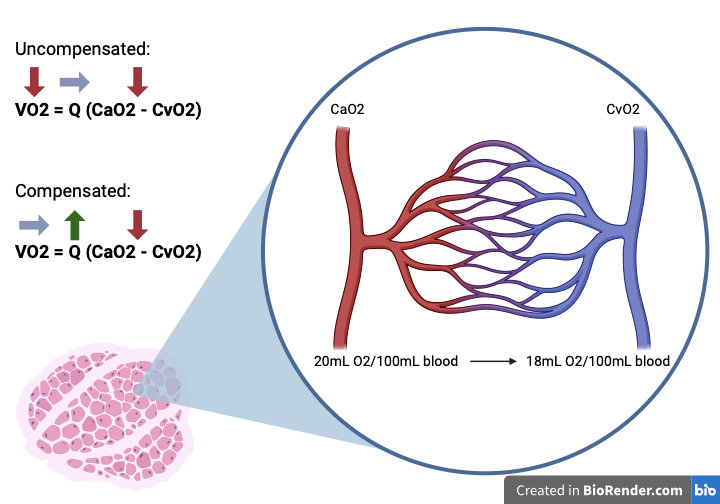
\includegraphics[width=0.5\linewidth]{Sarcopenia.png}
    \caption{Effect of Sarcopenia on avO2 Difference }
    \label{fig:enter-label}
\end{figure}

\textbf{Integrative Exercise: Adaptive Changes in Patients with Anemia }
Use Fick’s Equation to explain the adaptive changes seen in anemic patients.

Anemia is described as a decrease in red blood cell parameters (e.g. RBC count, hemoglobin, hematocrit). Arising from two primary mechanisms: (1) decreased red blood cell production or (2) increased red blood cell loss, anemia can result in cell hypoxia and if severe, tissue anoxia with subsequent cell death. Clinically, patient's with anemia may present with increased baseline levels of fatigue, weakness, tachycardia, and dyspnea.

As previously stated in the text, hemoglobin is a protein present in the RBC’s, which enables the binding and transportation of oxygen to relevant areas of need (both peripheral and visceral tissue). As anemia progresses there is a gradual decline in the blood’s ability to meet the oxygen demands of the tissue. To meet the oxygen demands of the tissue, multi-system compensations are seen. Short term compensations may arise in the form of tachycardia, which would pump more blood (mL) per unit of time in an attempt to adjust for the decrease in oxygenated blood. This increase in heart rate would contribute to an increase in stroke volume and thus, cardiac output. Although this compensatory mechanism may assist in managing local ischemia in the short term, the long term consequences of a chronic increase in cardiac output has significant implications. 



Anemia, which results in low RBC

May clinically present with pallor, increased baseline levels of fatigue, and dyspnea. 

Increased physical activity increases the demand for oxygen. 

Chronic anemia, greater need for oxygen systemically may result in cardiac output increases, but an inverse relationship with exercise tolerance. 

\begin{itemize}
    \item Low CO: hypovolemia, hypoperfusion, shock, arrhythmia, severe metabolic acidosis 
    \item High CO: hypoxia, use of positive inotropy, anemia 
    \item Low SV: High SV: bradycardia, the use of positive inotropes, decreases in afterload 
\end{itemize}


An example provided earlier in the chapter outlined the normal physiologic response to a supine to sit transfer. 

Summary: 




\section{Attain-Sustain Spectrum}

The attain-sustain spectrum in the context of Fick's equation can be described as the relationship between oxygen delivery and oxygen consumption in which the metabolic demands of the tissues are initially met, and then subsequently continued at levels physiologically safe. 

attain - achieving of threshold
sustain 

The body's ultimate goal is preservation of this balance between oxygen delivery and oxygen consumption. 

Fick's equation gives the physical therapist improved insight as it relates to overall understanding of cardiac function, principally, oxygen consumption, flow rate, and arterovenous difference. 

\printbibliography[heading=subbibintoc]
%% !TEX root = ../notes_template.tex
\chapter{Exercise Prescription}\label{chp:ex_prescription}
Updated on \today
\minitoc


\printbibliography[heading=subbibintoc]

\backmatter%%%%%%%%%%%%%%%%%%%%%%%%%%%%%%%%%%%%%%%%%%%%%%%%%%%%%%%
\Extrachap{Next Steps}

There are several next steps to this book. This is not even a first edition. This is a pre-edition, a third draft of what will be a completed book. One thing is clear though - it will always be a self-published, no cost (eBook) or low cost (printing cost only) textbook. Though as the pages increase the cost for pages will increase. But no fear. If you've purchased this draft, keep it and if a new draft or when the first edition is printed, I'll give you a new printed copy \textit{gratis}. 

\subsection*{New Content}

\textbf{Chapter 13 - Digestion, Absorption and Metabolism} is currently a missing but necessary chapter for \textbf{Part III} on Muscle Support. Without food and water entering the body, being digested, absorbed and metabolized the extra-cellular fluid cannot sustain muscle fibers. It has not been written yet because - at least at Plymouth State University DPT - it is not part of the first Clinical Physiology course. It is taught in the Nutrition and Exercise Prescription course. It is forthcoming and in progress. It sits at the border of Part III on muscle support and Part IV on the maintenance of long term muscle cell health, growth and repair.

\textbf{Part IV} is currently in process and focuses on muscle molecular biology. Specifically, how the muscle continues to fulfill its role of creating tension without being too large of a burden on the physiological support systems. Topics include maintaining muscle cells and tissue for the demands they are placed under through the processes of atrophy, hypertrophy, and repair. 

\textbf{Part V} is also in process and will include a variety of integrated exercises. These topics have been selected to highlight the need for physiological coordination such as Fick's Equation to highlight integration of the material in Parts II and III; exercise prescription and antigravity, cold and hypoxia exposure to highlight integration of the material in Parts II, III and IV; the autonomic nervous system to highlight integration of Parts III and IV; and rehabilitation protocols to highlight integration of Part I with the all other parts as the full spectrum of hierarchy is manifest in clinical practice.

Clinical practice is a fulfillment of clinical physiology. Practice abductively reasons based on physiology to understand movement problems; and practice attempts to deductively modify physiology through interventions.

\subsection*{Update Content}

It is hoped that all of the typos, errors and mishaps in the existing content will be fixed prior to the final publication of the first edition of the text. There are still some rather long and muddy sections that require at least one more pass through in the tried and tested locale of classroom teaching and student feedback!

\subsection*{Added Features}

Additional features for the first edition will be the inclusion of a glossary of key terms at the end of each chapter, and an index at the end of the book. In all honesty, I really need a full printed draft to highlight those terms worty of being in the glossary and the index.
Finally, an end of book Works Cited page is necessary for those - like me - that enjoy reading through the works cited in masse and not just by chapter. This feature will not remove the end of chapter references because both are options worthy of inclusion for different preferences.

%\include{author/glossary}
%\include{author/solutions}
%\printindex

%%%%%%%%%%%%%%%%%%%%%%%%%%%%%%%%%%%%%%%%%%%%%%%%%%%%%%%%%%%%%%%%%%%%%%

\end{document}





